%&preformat-disser
\RequirePackage[l2tabu,orthodox]{nag} % Раскомментировав, можно в логе получать рекомендации относительно правильного использования пакетов и предупреждения об устаревших и нерекомендуемых пакетах
% Формат А4, 14pt (ГОСТ Р 7.0.11-2011, 5.3.6)
\documentclass[a4paper,14pt,oneside,openany]{memoir}

%% Режим черновика
\makeatletter
\@ifundefined{c@draft}{
  \newcounter{draft}
  \setcounter{draft}{0}  % 0 --- чистовик (максимальное соблюдение ГОСТ)
                         % 1 --- черновик (отклонения от ГОСТ, но быстрая сборка итоговых PDF)
}{}
\makeatother

%% Библиография

%% Внимание! При использовании bibtex8 необходимо удалить все
%% цитирования из  ../common/characteristic.tex
\newcounter{bibliosel}
\setcounter{bibliosel}{1}           % 0 --- встроенная реализация с загрузкой файла через движок bibtex8; 1 --- реализация пакетом biblatex через движок biber
               % общие настройки шаблона
%%% Проверка используемого TeX-движка %%%
\usepackage{iftex}[2013/04/04]
\newif\ifxetexorluatex   % определяем новый условный оператор (http://tex.stackexchange.com/a/47579/79756)
\ifXeTeX
    \xetexorluatextrue
\else
    \ifLuaTeX
        \xetexorluatextrue
    \else
        \xetexorluatexfalse
    \fi
\fi

\RequirePackage{etoolbox}[2015/08/02]               % Для продвинутой проверки разных условий

%%% Поля и разметка страницы %%%
\usepackage{pdflscape}                              % Для включения альбомных страниц
\usepackage{geometry}                               % Для последующего задания полей

%%% Математические пакеты %%%
\usepackage{amsthm,amsfonts,amsmath,amssymb,amscd}  % Математические дополнения от AMS
\usepackage{mathtools}                              % Добавляет окружение multlined

%%%% Установки для размера шрифта 14 pt %%%%
%% Формирование переменных и констант для сравнения (один раз для всех подключаемых файлов)%%
%% должно располагаться до вызова пакета fontspec или polyglossia, потому что они сбивают его работу
\newlength{\curtextsize}
\newlength{\bigtextsize}
\setlength{\bigtextsize}{13.9pt}

\makeatletter
%\show\f@size                                       % неплохо для отслеживания, но вызывает стопорение процесса, если документ компилируется без команды  -interaction=nonstopmode 
\setlength{\curtextsize}{\f@size pt}
\makeatother

%%% Кодировки и шрифты %%%
\ifxetexorluatex
    \usepackage{polyglossia}[2014/05/21]            % Поддержка многоязычности (fontspec подгружается автоматически)
\else
    \RequirePDFTeX                                  % tests for PDFTEX use and throws an error if a different engine is being used
   %%% Решение проблемы копирования текста в буфер кракозябрами
%    \input glyphtounicode.tex
%    \input glyphtounicode-cmr.tex %from pdfx package
%    \pdfgentounicode=1
    \usepackage{cmap}                               % Улучшенный поиск русских слов в полученном pdf-файле
    \defaulthyphenchar=127                          % Если стоит до fontenc, то переносы не впишутся в выделяемый текст при копировании его в буфер обмена
    \usepackage[T2A]{fontenc}                       % Поддержка русских букв
    \usepackage[utf8]{inputenc}[2014/04/30]         % Кодировка utf8
    \usepackage[english, russian]{babel}[2014/03/24]% Языки: русский, английский
    \IfFileExists{pscyr.sty}{\usepackage{pscyr}}{}  % Красивые русские шрифты
\fi

%%% Оформление абзацев %%%
\usepackage{indentfirst}                            % Красная строка

%%% Цвета %%%
\usepackage[dvipsnames,usenames]{color}
\usepackage{colortbl}
%\usepackage[dvipsnames, table, hyperref, cmyk]{xcolor} % Вероятно, более новый вариант, вместо предыдущих двух строк. Конвертация всех цветов в cmyk заложена как удовлетворение возможного требования типографий. Возможно конвертирование и в rgb.

%%% Таблицы %%%
\usepackage{longtable}                              % Длинные таблицы
\usepackage{multirow,makecell}                      % Улучшенное форматирование таблиц

%%% Общее форматирование
\usepackage{soulutf8}                               % Поддержка переносоустойчивых подчёркиваний и зачёркиваний
\usepackage{icomma}                                 % Запятая в десятичных дробях


%%% Гиперссылки %%%
\usepackage{hyperref}[2012/11/06]

%%% Изображения %%%
\usepackage{graphicx}[2014/04/25]                   % Подключаем пакет работы с графикой

%%% Списки %%%
\usepackage{enumitem}

%%% Подписи %%%
\usepackage{caption}[2013/05/02]                    % Для управления подписями (рисунков и таблиц) % Может управлять номерами рисунков и таблиц с caption %Иногда может управлять заголовками в списках рисунков и таблиц
\usepackage{subcaption}[2013/02/03]                 % Работа с подрисунками и подобным

%%% Счётчики %%%
\usepackage[figure,table]{totalcount}               % Счётчик рисунков и таблиц
\usepackage{totcount}                               % Пакет создания счётчиков на основе последнего номера подсчитываемого элемента (может требовать дважды компилировать документ)
\usepackage{totpages}                               % Счётчик страниц, совместимый с hyperref (ссылается на номер последней страницы). Желательно ставить последним пакетом в преамбуле

%%% Продвинутое управление групповыми ссылками (пока только формулами) %%%
\ifxetexorluatex
    \usepackage{cleveref}                           % cleveref корректно считывает язык из настроек polyglossia
\else
    \usepackage[russian]{cleveref}                  % cleveref имеет сложности со считыванием языка из babel. Такое решение русификации вывода выбрано вместо определения в documentclass из опасности что-то лишнее передать во все остальные пакеты, включая библиографию.
\fi
\creflabelformat{equation}{#2#1#3}                  % Формат по умолчанию ставил круглые скобки вокруг каждого номера ссылки, теперь просто номера ссылок без какого-либо дополнительного оформления


\ifnumequal{\value{draft}}{1}{% Черновик
    \usepackage[firstpage]{draftwatermark}
    \SetWatermarkText{DRAFT}
    \SetWatermarkFontSize{14pt}
    \SetWatermarkScale{15}
    \SetWatermarkAngle{45}
}{}

  % Пакеты общие для диссертации и автореферата
%%% Прикладные пакеты %%%
%\usepackage{calc}               % Пакет для расчётов параметров, например длины

%%% Для добавления Стр. над номерами страниц в оглавлении
%%% http://tex.stackexchange.com/a/306950
\usepackage{afterpage}

% \hyp{}
\usepackage{hyphenat}
         % Пакеты для диссертации
\usepackage{tabu, tabulary}  %таблицы с автоматически подбирающейся шириной столбцов
\usepackage{fr-longtable}    %ради \endlasthead

% Листинги с исходным кодом программ
\usepackage{fancyvrb}
\usepackage{listings}
\lccode`\~=0\relax %Без этого хака из-за особенностей пакета listings перестают работать конструкции с \MakeLowercase и т. п. в (xe|lua)latex

% Русская традиция начертания греческих букв
\usepackage{upgreek} % прямые греческие ради русской традиции

% Микротипографика
%\ifnumequal{\value{draft}}{0}{% Только если у нас режим чистовика
%    \usepackage[final]{microtype}[2016/05/14] % улучшает представление букв и слов в строках, может помочь при наличии отдельно висящих слов
%}{}

% Отметка о версии черновика на каждой странице
% Чтобы работало надо в своей локальной копии по инструкции
% https://www.ctan.org/pkg/gitinfo2 создать небходимые файлы в папке
% ./git/hooks
% If you’re familiar with tweaking git, you can probably work it out for
% yourself. If not, I suggest you follow these steps:
% 1. First, you need a git repository and working tree. For this example,
% let’s suppose that the root of the working tree is in ~/compsci
% 2. Copy the file post-xxx-sample.txt (which is in the same folder of
% your TEX distribution as this pdf) into the git hooks directory in your
% working copy. In our example case, you should end up with a file called
% ~/compsci/.git/hooks/post-checkout
% 3. If you’re using a unix-like system, don’t forget to make the file executable.
% Just how you do this is outside the scope of this manual, but one
% possible way is with commands such as this:
% chmod g+x post-checkout.
% 4. Test your setup with “git checkout master” (or another suitable branch
% name). This should generate copies of gitHeadInfo.gin in the directories
% you intended.
% 5. Now make two more copies of this file in the same directory (hooks),
% calling them post-commit and post-merge, and you’re done. As before,
% users of unix-like systems should ensure these files are marked as
% executable.
\ifnumequal{\value{draft}}{1}{% Черновик
   \IfFileExists{.git/gitHeadInfo.gin}{
      \usepackage[mark,pcount]{gitinfo2}
      \renewcommand{\gitMark}{rev.\gitAbbrevHash\quad\gitCommitterEmail\quad\gitAuthorIsoDate}
      \renewcommand{\gitMarkFormat}{\color{Gray}\small\bfseries}
   }{}
}{}

% For colors in pdf compiled from svg.
\usepackage{xcolor}
% \hyp{}
\usepackage{hyphenat}

% Package for drawing
\usepackage{tikz}
\usetikzlibrary{snakes,arrows,shapes}
        % Пакеты для специфических пользовательских задач

%%%%%%%%%%%%%%%%%%%%%%%%%%%%%%%%%%%%%%%%%%%%%%%%%%%%%%
%%%% Файл упрощённых настроек шаблона диссертации %%%%
%%%%%%%%%%%%%%%%%%%%%%%%%%%%%%%%%%%%%%%%%%%%%%%%%%%%%%

%%% Инициализирование переменных, не трогать!  %%%
\newcounter{intvl}
\newcounter{otstup}
\newcounter{contnumeq}
\newcounter{contnumfig}
\newcounter{contnumtab}
\newcounter{pgnum}
\newcounter{chapstyle}
\newcounter{headingdelim}
\newcounter{headingalign}
\newcounter{headingsize}
\newcounter{tabcap}
\newcounter{tablaba}
\newcounter{tabtita}
%%%%%%%%%%%%%%%%%%%%%%%%%%%%%%%%%%%%%%%%%%%%%%%%%%

%%% Область упрощённого управления оформлением %%%

%% Интервал между заголовками и между заголовком и текстом
% Заголовки отделяют от текста сверху и снизу тремя интервалами (ГОСТ Р 7.0.11-2011, 5.3.5)
\setcounter{intvl}{3}               % Коэффициент кратности к размеру шрифта

%% Отступы у заголовков в тексте
\setcounter{otstup}{0}              % 0 --- без отступа; 1 --- абзацный отступ

%% Нумерация формул, таблиц и рисунков
\setcounter{contnumeq}{0}           % Нумерация формул: 0 --- пораздельно (во введении подряд, без номера раздела); 1 --- сквозная нумерация по всей диссертации
\setcounter{contnumfig}{0}          % Нумерация рисунков: 0 --- пораздельно (во введении подряд, без номера раздела); 1 --- сквозная нумерация по всей диссертации
\setcounter{contnumtab}{1}          % Нумерация таблиц: 0 --- пораздельно (во введении подряд, без номера раздела); 1 --- сквозная нумерация по всей диссертации

%% Оглавление
\setcounter{pgnum}{1}               % 0 --- номера страниц никак не обозначены; 1 --- Стр. над номерами страниц (дважды компилировать после изменения)
\settocdepth{subsection}            % до какого уровня подразделов выносить в оглавление
\setsecnumdepth{subsection}         % до какого уровня нумеровать подразделы


%% Текст и форматирование заголовков
\setcounter{chapstyle}{1}           % 0 --- разделы только под номером; 1 --- разделы с названием "Глава" перед номером
\setcounter{headingdelim}{1}        % 0 --- номер отделен пропуском в 1em или \quad; 1 --- номера разделов и приложений отделены точкой с пробелом, подразделы пропуском без точки; 2 --- номера разделов, подразделов и приложений отделены точкой с пробелом.

%% Выравнивание заголовков в тексте
\setcounter{headingalign}{0}        % 0 --- по центру; 1 --- по левому краю

%% Размеры заголовков в тексте
\setcounter{headingsize}{0}         % 0 --- по ГОСТ, все всегда 14 пт; 1 --- пропорционально изменяющийся размер в зависимости от базового шрифта

%% Подпись таблиц
\setcounter{tabcap}{0}              % 0 --- по ГОСТ, номер таблицы и название разделены тире, выровнены по левому краю, при необходимости на нескольких строках; 1 --- подпись таблицы не по ГОСТ, на двух и более строках, дальнейшие настройки: 
%Выравнивание первой строки, с подписью и номером
\setcounter{tablaba}{2}             % 0 --- по левому краю; 1 --- по центру; 2 --- по правому краю
%Выравнивание строк с самим названием таблицы
\setcounter{tabtita}{1}             % 0 --- по левому краю; 1 --- по центру; 2 --- по правому краю
%Разделитель записи «Таблица #» и названия таблицы
\newcommand{\tablabelsep}{space}   % space = пробел, period = точка (определены в подключенных пакетах)

%% Подпись рисунков
%Разделитель записи «Рисунок #» и названия рисунка
\newcommand{\figlabelsep}{emdash}   % emdash = тире, определён в common/styles; period = точка определён в подключенных пакетах

%%% Цвета гиперссылок %%%
% Latex color definitions: http://latexcolor.com/
\definecolor{linkcolor}{rgb}{0.9,0,0}
\definecolor{citecolor}{rgb}{0,0.6,0}
\definecolor{urlcolor}{rgb}{0,0,1}
%\definecolor{linkcolor}{rgb}{0,0,0} %black
%\definecolor{citecolor}{rgb}{0,0,0} %black
%\definecolor{urlcolor}{rgb}{0,0,0} %black               % Упрощённые настройки шаблона

%%% Переопределение именований, чтобы можно было и в преамбуле использовать %%%
\renewcommand{\chaptername}{Глава}
\renewcommand{\appendixname}{Приложение} % (ГОСТ Р 7.0.11-2011, 5.7)
       % Переопределение именований, чтобы можно было и в преамбуле использовать
% Новые переменные, которые могут использоваться во всём проекте
% ГОСТ 7.0.11-2011
% 9.2 Оформление текста автореферата диссертации
% 9.2.1 Общая характеристика работы включает в себя следующие основные структурные
% элементы:
% актуальность темы исследования;
\newcommand{\actualityTXT}{Актуальность темы.}
% степень ее разработанности;
\newcommand{\progressTXT}{Степень разработанности темы.}
% цели и задачи;
\newcommand{\aimTXT}{Целью}
\newcommand{\tasksTXT}{задачи}
% научную новизну;
\newcommand{\noveltyTXT}{Научная новизна:}
% теоретическую и практическую значимость работы;
%\newcommand{\influenceTXT}{Теоретическая и практическая значимость}
% или чаще используют просто
\newcommand{\influenceTXT}{Практическая значимость}
% методологию и методы исследования;
\newcommand{\methodsTXT}{Mетодология и методы исследования.}
% положения, выносимые на защиту;
\newcommand{\defpositionsTXT}{Основные положения, выносимые на~защиту:}
% степень достоверности и апробацию результатов.
\newcommand{\reliabilityTXT}{Достоверность}
\newcommand{\probationTXT}{Апробация работы.}

\newcommand{\contributionTXT}{Личный вклад.}
\newcommand{\publicationsTXT}{Публикации.}


\newcommand{\authorbibtitle}{Публикации автора по теме диссертации}
\newcommand{\vakbibtitle}{В изданиях из списка ВАК РФ}
\newcommand{\notvakbibtitle}{В прочих изданиях}
\newcommand{\confbibtitle}{В сборниках трудов конференций}
\newcommand{\fullbibtitle}{Список литературы} % (ГОСТ Р 7.0.11-2011, 4)
  % Новые переменные, которые могут использоваться во всём проекте

%%% Основные сведения %%%
\newcommand{\thesisAuthor}             % Диссертация, ФИО автора
{%
    \texorpdfstring{% \texorpdfstring takes two arguments and uses the first for (La)TeX and the second for pdf
        Новиков Александр Витальевич% так будет отображаться на титульном листе или в тексте, где будет использоваться переменная
    }{%
        Новиков Александр Витальевич% эта запись для свойств pdf-файла. В таком виде, если pdf будет обработан программами для сбора библиографических сведений, будет правильно представлена фамилия.
    }%
}
\newcommand{\thesisAuthorShort}        % Диссертация, ФИО автора инициалами
{\todo{А.В.~Новиков}}

%\newcommand{\thesisUdk}                % Диссертация, УДК
%{\todo{xxx.xxx}}
\newcommand{\thesisTitle}              % Диссертация, название
{\texorpdfstring{\MakeUppercase{Тензорные методы в задачах распознавания образов}}{Название диссертационной работы}}
\newcommand{\thesisSpecialtyNumber}    % Диссертация, специальность, номер
{\texorpdfstring{05.13.18}{05.13.18}}
\newcommand{\thesisSpecialtyTitle}     % Диссертация, специальность, название
{\texorpdfstring{Математическое моделирование, численные методы и комплексы программ}{Математическое моделирование, численные методы и комплексы программ}}
\newcommand{\thesisDegree}             % Диссертация, ученая степень
{кандидата физико-математических наук}
\newcommand{\thesisDegreeShort}        % Диссертация, ученая степень, краткая запись
{канд. физ.-мат. наук}
\newcommand{\thesisCity}               % Диссертация, город написания диссертации
{Москва}
\newcommand{\thesisYear}               % Диссертация, год написания диссертации
{2018}
\newcommand{\thesisOrganization}       % Диссертация, организация
{ФЕДЕРАЛЬНОЕ ГОСУДАРСТВЕННОЕ БЮДЖЕТНОЕ УЧРЕЖДЕНИЕ НАУКИ ИНСТИТУТ ВЫЧИСЛИТЕЛЬНОЙ МАТЕМАТИКИ РОССИЙСКОЙ АКАДЕМИИ НАУК}
\newcommand{\thesisOrganizationShort}  % Диссертация, краткое название организации для доклада
{\todo{НазУчДисРаб}}

\newcommand{\thesisInOrganization}     % Диссертация, организация в предложном падеже: Работа выполнена в ...
{\todo{учреждении, в~котором выполнялась данная диссертационная работа}}

\newcommand{\supervisorFio}            % Научный руководитель, ФИО
{Оселедец И. В.}
\newcommand{\supervisorRegalia}        % Научный руководитель, регалии
{д.ф.-м.н. }
\newcommand{\supervisorFioShort}       % Научный руководитель, ФИО
{И.В.~Оселедец}
\newcommand{\supervisorRegaliaShort}   % Научный руководитель, регалии
{\todo{уч.~ст.,~уч.~зв.}}

\newcommand{\cosupervisorFio}            % Научный руководитель, ФИО
{Ветров Д.П.}
\newcommand{\cosupervisorRegalia}        % Научный руководитель, регалии
{к.ф.-м.н. }


\newcommand{\opponentOneFio}           % Оппонент 1, ФИО
{\todo{Фамилия Имя Отчество}}
\newcommand{\opponentOneRegalia}       % Оппонент 1, регалии
{\todo{доктор физико-математических наук, профессор}}
\newcommand{\opponentOneJobPlace}      % Оппонент 1, место работы
{\todo{Не очень длинное название для места работы}}
\newcommand{\opponentOneJobPost}       % Оппонент 1, должность
{\todo{старший научный сотрудник}}

\newcommand{\opponentTwoFio}           % Оппонент 2, ФИО
{\todo{Фамилия Имя Отчество}}
\newcommand{\opponentTwoRegalia}       % Оппонент 2, регалии
{\todo{кандидат физико-математических наук}}
\newcommand{\opponentTwoJobPlace}      % Оппонент 2, место работы
{\todo{Основное место работы c длинным длинным длинным длинным названием}}
\newcommand{\opponentTwoJobPost}       % Оппонент 2, должность
{\todo{старший научный сотрудник}}

\newcommand{\leadingOrganizationTitle} % Ведущая организация, дополнительные строки
{\todo{Федеральное государственное бюджетное образовательное учреждение высшего профессионального образования с~длинным длинным длинным длинным названием}}

\newcommand{\defenseDate}              % Защита, дата
{\todo{DD mmmmmmmm YYYY~г.~в~XX часов}}
\newcommand{\defenseCouncilNumber}     % Защита, номер диссертационного совета
{\todo{Д\,123.456.78}}
\newcommand{\defenseCouncilTitle}      % Защита, учреждение диссертационного совета
{\todo{Название учреждения}}
\newcommand{\defenseCouncilAddress}    % Защита, адрес учреждение диссертационного совета
{\todo{Адрес}}
\newcommand{\defenseCouncilPhone}      % Телефон для справок
{\todo{+7~(0000)~00-00-00}}

\newcommand{\defenseSecretaryFio}      % Секретарь диссертационного совета, ФИО
{\todo{Фамилия Имя Отчество}}
\newcommand{\defenseSecretaryRegalia}  % Секретарь диссертационного совета, регалии
{\todo{д-р~физ.-мат. наук}}            % Для сокращений есть ГОСТы, например: ГОСТ Р 7.0.12-2011 + http://base.garant.ru/179724/#block_30000

\newcommand{\synopsisLibrary}          % Автореферат, название библиотеки
{\todo{Название библиотеки}}
\newcommand{\synopsisDate}             % Автореферат, дата рассылки
{\todo{DD mmmmmmmm YYYY года}}

% To avoid conflict with beamer class use \providecommand
\providecommand{\keywords}%            % Ключевые слова для метаданных PDF диссертации и автореферата
{}
      % Основные сведения
%%% Кодировки и шрифты %%%
\ifxetexorluatex
    \setmainlanguage[babelshorthands=true]{russian}  % Язык по-умолчанию русский с поддержкой приятных команд пакета babel
    \setotherlanguage{english}                       % Дополнительный язык = английский (в американской вариации по-умолчанию)
    \setmonofont{Courier New}
    \newfontfamily\cyrillicfonttt{Courier New}
    \ifXeTeX
        \defaultfontfeatures{Ligatures=TeX,Mapping=tex-text}
    \else
        \defaultfontfeatures{Ligatures=TeX}
    \fi
    \setmainfont{Times New Roman}
    \newfontfamily\cyrillicfont{Times New Roman}
    \setsansfont{Arial}
    \newfontfamily\cyrillicfontsf{Arial}
\else
    \IfFileExists{pscyr.sty}{\renewcommand{\rmdefault}{ftm}}{}
\fi

%%% Подписи %%%
\captionsetup{%
singlelinecheck=off,                % Многострочные подписи, например у таблиц
skip=2pt,                           % Вертикальная отбивка между подписью и содержимым рисунка или таблицы определяется ключом
justification=centering,            % Центрирование подписей, заданных командой \caption
}

%%% Рисунки %%%
\DeclareCaptionLabelSeparator*{emdash}{~--- }             % (ГОСТ 2.105, 4.3.1)
\captionsetup[figure]{labelsep=\figlabelsep,position=bottom}

%%% Таблицы %%%
\ifnumequal{\value{tabcap}}{0}{%
    \newcommand{\tabcapalign}{\raggedright}  % по левому краю страницы или аналога parbox

    \DeclareCaptionFormat{tablecaption}{\tabcapalign #1#2#3}
    \captionsetup[table]{labelsep=emdash}        % тире как разделитель идентификатора с номером от наименования
}{%
    \ifnumequal{\value{tablaba}}{0}{%
        \newcommand{\tabcapalign}{\raggedright}  % по левому краю страницы или аналога parbox
    }{}

    \ifnumequal{\value{tablaba}}{1}{%
        \newcommand{\tabcapalign}{\centering}    % по центру страницы или аналога parbox
    }{}

    \ifnumequal{\value{tablaba}}{2}{%
        \newcommand{\tabcapalign}{\raggedleft}   % по правому краю страницы или аналога parbox
    }{}

    \ifnumequal{\value{tabtita}}{0}{%
        \newcommand{\tabtitalign}{\raggedright}  % по левому краю страницы или аналога parbox
    }{}

    \ifnumequal{\value{tabtita}}{1}{%
        \newcommand{\tabtitalign}{\centering}    % по центру страницы или аналога parbox
    }{}

    \ifnumequal{\value{tabtita}}{2}{%
        \newcommand{\tabtitalign}{\raggedleft}   % по правому краю страницы или аналога parbox
    }{}

    \DeclareCaptionFormat{tablecaption}{\tabcapalign #1#2\par%  % Идентификатор таблицы на отдельной строке
        \tabtitalign{#3}}                                       % Наименование таблицы строкой ниже
    \captionsetup[table]{labelsep=\tablabelsep}                 % разделитель идентификатора с номером от наименования
}
\DeclareCaptionFormat{tablenocaption}{\tabcapalign #1\strut}    % Наименование таблицы отсутствует

\captionsetup[table]{format=tablecaption,singlelinecheck=off,position=top,skip=0pt}  % многострочные наименования и прочее
\DeclareCaptionLabelFormat{continued}{Продолжение таблицы~#2}

%%% Подписи подрисунков %%%
\renewcommand{\thesubfigure}{\asbuk{subfigure}}           % Буквенные номера подрисунков
\captionsetup[subfigure]{font={normalsize},               % Шрифт подписи названий подрисунков (не отличается от основного)
    labelformat=brace,                                    % Формат обозначения подрисунка
    justification=centering,                              % Выключка подписей (форматирование), один из вариантов            
}
%\DeclareCaptionFont{font12pt}{\fontsize{12pt}{13pt}\selectfont} % объявляем шрифт 12pt для использования в подписях, тут же надо интерлиньяж объявлять, если не наследуется
%\captionsetup[subfigure]{font={font12pt}}                 % Шрифт подписи названий подрисунков (всегда 12pt)

%%% Настройки гиперссылок %%%
\ifLuaTeX
    \hypersetup{
        unicode,                % Unicode encoded PDF strings
    }
\fi

\hypersetup{
    linktocpage=true,           % ссылки с номера страницы в оглавлении, списке таблиц и списке рисунков
%    linktoc=all,                % both the section and page part are links
%    pdfpagelabels=false,        % set PDF page labels (true|false)
    plainpages=false,           % Forces page anchors to be named by the Arabic form  of the page number, rather than the formatted form
    colorlinks,                 % ссылки отображаются раскрашенным текстом, а не раскрашенным прямоугольником, вокруг текста
    linkcolor={linkcolor},      % цвет ссылок типа ref, eqref и подобных
    citecolor={citecolor},      % цвет ссылок-цитат
    urlcolor={urlcolor},        % цвет гиперссылок
%    hidelinks,                  % Hide links (removing color and border)
    pdftitle={\thesisTitle},    % Заголовок
    pdfauthor={\thesisAuthor},  % Автор
    pdfsubject={\thesisSpecialtyNumber\ \thesisSpecialtyTitle},      % Тема
%    pdfcreator={Создатель},     % Создатель, Приложение
%    pdfproducer={Производитель},% Производитель, Производитель PDF
    pdfkeywords={\keywords},    % Ключевые слова
    pdflang={ru},
}
\ifnumequal{\value{draft}}{1}{% Черновик
    \hypersetup{
        draft,
    }
}{}

%%% Шаблон %%%
\DeclareRobustCommand{\todo}{\textcolor{red}}       % решаем проблему превращения названия цвета в результате \MakeUppercase, http://tex.stackexchange.com/a/187930/79756 , \DeclareRobustCommand protects \todo from expanding inside \MakeUppercase
\AtBeginDocument{%
    \setlength{\parindent}{2.5em}                   % Абзацный отступ. Должен быть одинаковым по всему тексту и равен пяти знакам (ГОСТ Р 7.0.11-2011, 5.3.7).
}

%%% Списки %%%
% Используем короткое тире (endash) для ненумерованных списков (ГОСТ 2.105-95, пункт 4.1.7, требует дефиса, но так лучше смотрится)
\renewcommand{\labelitemi}{\normalfont\bfseries{--}}

% Перечисление строчными буквами латинского алфавита (ГОСТ 2.105-95, 4.1.7)
%\renewcommand{\theenumi}{\alph{enumi}}
%\renewcommand{\labelenumi}{\theenumi)} 

% Перечисление строчными буквами русского алфавита (ГОСТ 2.105-95, 4.1.7)
\makeatletter
\AddEnumerateCounter{\asbuk}{\russian@alph}{щ}      % Управляем списками/перечислениями через пакет enumitem, а он 'не знает' про asbuk, потому 'учим' его
\makeatother
%\renewcommand{\theenumi}{\asbuk{enumi}} %первый уровень нумерации
%\renewcommand{\labelenumi}{\theenumi)} %первый уровень нумерации 
\renewcommand{\theenumii}{\asbuk{enumii}} %второй уровень нумерации
\renewcommand{\labelenumii}{\theenumii)} %второй уровень нумерации 
\renewcommand{\theenumiii}{\arabic{enumiii}} %третий уровень нумерации
\renewcommand{\labelenumiii}{\theenumiii)} %третий уровень нумерации 

\setlist{nosep,%                                    % Единый стиль для всех списков (пакет enumitem), без дополнительных интервалов.
    labelindent=\parindent,leftmargin=*%            % Каждый пункт, подпункт и перечисление записывают с абзацного отступа (ГОСТ 2.105-95, 4.1.8)
}
    % Стили общие для диссертации и автореферата
%%% Изображения %%%
\graphicspath{{images/}{Dissertation/images/}}         % Пути к изображениям

%%% Макет страницы %%%
% Выставляем значения полей (ГОСТ 7.0.11-2011, 5.3.7)
\geometry{a4paper,top=2cm,bottom=2cm,left=2.5cm,right=1cm,nofoot,nomarginpar} %,showframe
\setlength{\topskip}{0pt}   %размер дополнительного верхнего поля

%%% Интервалы %%%
%% По ГОСТ Р 7.0.11-2011, пункту 5.3.6 требуется полуторный интервал
%% Реализация средствами класса (на основе setspace) ближе к типографской классике.
%% И правит сразу и в таблицах (если со звёздочкой) 
%\DoubleSpacing*     % Двойной интервал
\OnehalfSpacing*    % Полуторный интервал
%\setSpacing{1.42}   % Полуторный интервал, подобный Ворду (возможно, стоит включать вместе с предыдущей строкой)

%%% Выравнивание и переносы %%%
%% http://tex.stackexchange.com/questions/241343/what-is-the-meaning-of-fussy-sloppy-emergencystretch-tolerance-hbadness
%% http://www.latex-community.org/forum/viewtopic.php?p=70342#p70342
\tolerance 1414
\hbadness 1414
\emergencystretch 1.5em % В случае проблем регулировать в первую очередь
\hfuzz 0.3pt
\vfuzz \hfuzz
%\raggedbottom
%\sloppy                 % Избавляемся от переполнений
\clubpenalty=10000      % Запрещаем разрыв страницы после первой строки абзаца
\widowpenalty=10000     % Запрещаем разрыв страницы после последней строки абзаца

%%% Блок управления параметрами для выравнивания заголовков в тексте %%%
\newlength{\otstuplen}
\setlength{\otstuplen}{\theotstup\parindent}
\ifnumequal{\value{headingalign}}{0}{% выравнивание заголовков в тексте
    \newcommand{\hdngalign}{\centering}                % по центру
    \newcommand{\hdngaligni}{}% по центру
    \setlength{\otstuplen}{0pt}
}{%
    \newcommand{\hdngalign}{}                 % по левому краю
    \newcommand{\hdngaligni}{\hspace{\otstuplen}}      % по левому краю
} % В обоих случаях вроде бы без переноса, как и надо (ГОСТ Р 7.0.11-2011, 5.3.5)

%%% Оглавление %%%
\renewcommand{\cftchapterdotsep}{\cftdotsep}                % отбивка точками до номера страницы начала главы/раздела

%% Переносить слова в заголовке не допускается (ГОСТ Р 7.0.11-2011, 5.3.5). Заголовки в оглавлении должны точно повторять заголовки в тексте (ГОСТ Р 7.0.11-2011, 5.2.3). Прямого указания на запрет переносов в оглавлении нет, но по той же логике невнесения искажений в смысл, лучше в оглавлении не переносить:
\setrmarg{2.55em plus1fil}                             %To have the (sectional) titles in the ToC, etc., typeset ragged right with no hyphenation
\renewcommand{\cftchapterpagefont}{\normalfont}        % нежирные номера страниц у глав в оглавлении
\renewcommand{\cftchapterleader}{\cftdotfill{\cftchapterdotsep}}% нежирные точки до номеров страниц у глав в оглавлении
%\renewcommand{\cftchapterfont}{}                       % нежирные названия глав в оглавлении

\ifnumgreater{\value{headingdelim}}{0}{%
    \renewcommand\cftchapteraftersnum{.\space}       % добавляет точку с пробелом после номера раздела в оглавлении
}{}
\ifnumgreater{\value{headingdelim}}{1}{%
    \renewcommand\cftsectionaftersnum{.\space}       % добавляет точку с пробелом после номера подраздела в оглавлении
    \renewcommand\cftsubsectionaftersnum{.\space}    % добавляет точку с пробелом после номера подподраздела в оглавлении
    \renewcommand\cftsubsubsectionaftersnum{.\space} % добавляет точку с пробелом после номера подподподраздела в оглавлении
    \AtBeginDocument{% без этого polyglossia сама всё переопределяет
        \setsecnumformat{\csname the#1\endcsname.\space}
    }
}{%
    \AtBeginDocument{% без этого polyglossia сама всё переопределяет
        \setsecnumformat{\csname the#1\endcsname\quad}
    }
}

\renewcommand*{\cftappendixname}{\appendixname\space} % Слово Приложение в оглавлении

%%% Колонтитулы %%%
% Порядковый номер страницы печатают на середине верхнего поля страницы (ГОСТ Р 7.0.11-2011, 5.3.8)
\makeevenhead{plain}{}{\thepage}{}
\makeoddhead{plain}{}{\thepage}{}
\makeevenfoot{plain}{}{}{}
\makeoddfoot{plain}{}{}{}
\pagestyle{plain}

%%% добавить Стр. над номерами страниц в оглавлении
%%% http://tex.stackexchange.com/a/306950
\newif\ifendTOC

\newcommand*{\tocheader}{
\ifnumequal{\value{pgnum}}{1}{%
    \ifendTOC\else\hbox to \linewidth%
      {\noindent{}~\hfill{Стр.}}\par%
      \ifnumless{\value{page}}{3}{}{%
        \vspace{0.5\onelineskip}
      }
      \afterpage{\tocheader}
    \fi%
}{}%
}%

%%% Оформление заголовков глав, разделов, подразделов %%%
%% Работа должна быть выполнена ... размером шрифта 12-14 пунктов (ГОСТ Р 7.0.11-2011, 5.3.8). То есть не должно быть надписей шрифтом более 14. Так и поставим.
%% Эти установки будут давать одинаковый результат независимо от выбора базовым шрифтом 12 пт или 14 пт
\newcommand{\basegostsectionfont}{\fontsize{14pt}{16pt}\selectfont\bfseries}

\makechapterstyle{thesisgost}{%
    \chapterstyle{default}
    \setlength{\beforechapskip}{0pt}
    \setlength{\midchapskip}{0pt}
    \setlength{\afterchapskip}{\theintvl\curtextsize}
    \renewcommand*{\chapnamefont}{\basegostsectionfont}
    \renewcommand*{\chapnumfont}{\basegostsectionfont}
    \renewcommand*{\chaptitlefont}{\basegostsectionfont}
    \renewcommand*{\chapterheadstart}{}
    \ifnumgreater{\value{headingdelim}}{0}{%
        \renewcommand*{\afterchapternum}{.\space}   % добавляет точку с пробелом после номера раздела
    }{%
        \renewcommand*{\afterchapternum}{\quad}     % добавляет \quad после номера раздела
    }
    \renewcommand*{\printchapternum}{\hdngaligni\hdngalign\chapnumfont \thechapter}
    \renewcommand*{\printchaptername}{}
    \renewcommand*{\printchapternonum}{\hdngaligni\hdngalign}
}

\makeatletter
\makechapterstyle{thesisgostchapname}{%
    \chapterstyle{thesisgost}
    \renewcommand*{\printchapternum}{\chapnumfont \thechapter}
    \renewcommand*{\printchaptername}{\hdngaligni\hdngalign\chapnamefont \@chapapp} %
}
\makeatother

\chapterstyle{thesisgost}

\setsecheadstyle{\basegostsectionfont\hdngalign}
\setsecindent{\otstuplen}

\setsubsecheadstyle{\basegostsectionfont\hdngalign}
\setsubsecindent{\otstuplen}

\setsubsubsecheadstyle{\basegostsectionfont\hdngalign}
\setsubsubsecindent{\otstuplen}

\sethangfrom{\noindent #1} %все заголовки подразделов центрируются с учетом номера, как block 

\ifnumequal{\value{chapstyle}}{1}{%
    \chapterstyle{thesisgostchapname}
    \renewcommand*{\cftchaptername}{\chaptername\space} % будет вписано слово Глава перед каждым номером раздела в оглавлении
}{}%

%%% Интервалы между заголовками
\setbeforesecskip{\theintvl\curtextsize}% Заголовки отделяют от текста сверху и снизу тремя интервалами (ГОСТ Р 7.0.11-2011, 5.3.5).
\setaftersecskip{\theintvl\curtextsize}
\setbeforesubsecskip{\theintvl\curtextsize}
\setaftersubsecskip{\theintvl\curtextsize}
\setbeforesubsubsecskip{\theintvl\curtextsize}
\setaftersubsubsecskip{\theintvl\curtextsize}

%%% Блок дополнительного управления размерами заголовков
\ifnumequal{\value{headingsize}}{1}{% Пропорциональные заголовки и базовый шрифт 14 пт
    \renewcommand{\basegostsectionfont}{\large\bfseries}
    \renewcommand*{\chapnamefont}{\Large\bfseries}
    \renewcommand*{\chapnumfont}{\Large\bfseries}
    \renewcommand*{\chaptitlefont}{\Large\bfseries}
}{}

%%% Счётчики %%%

%% Упрощённые настройки шаблона диссертации: нумерация формул, таблиц, рисунков
\ifnumequal{\value{contnumeq}}{1}{%
    \counterwithout{equation}{chapter} % Убираем связанность номера формулы с номером главы/раздела
}{}
\ifnumequal{\value{contnumfig}}{1}{%
    \counterwithout{figure}{chapter}   % Убираем связанность номера рисунка с номером главы/раздела
}{}
\ifnumequal{\value{contnumtab}}{1}{%
    \counterwithout{table}{chapter}    % Убираем связанность номера таблицы с номером главы/раздела
}{}


%%http://www.linux.org.ru/forum/general/6993203#comment-6994589 (используется totcount)
\makeatletter
\def\formbytotal#1#2#3#4#5{%
    \newcount\@c
    \@c\totvalue{#1}\relax
    \newcount\@last
    \newcount\@pnul
    \@last\@c\relax
    \divide\@last 10
    \@pnul\@last\relax
    \divide\@pnul 10
    \multiply\@pnul-10
    \advance\@pnul\@last
    \multiply\@last-10
    \advance\@last\@c
    \total{#1}~#2%
    \ifnum\@pnul=1#5\else%
    \ifcase\@last#5\or#3\or#4\or#4\or#4\else#5\fi
    \fi
}
\makeatother

\AtBeginDocument{
%% регистрируем счётчики в системе totcounter
    \regtotcounter{totalcount@figure}
    \regtotcounter{totalcount@table}       % Если иным способом поставить в преамбуле то ошибка в числе таблиц
    \regtotcounter{TotPages}               % Если иным способом поставить в преамбуле то ошибка в числе страниц
}

%%% Правильная нумерация приложений %%%
%% По ГОСТ 2.105, п. 4.3.8 Приложения обозначают заглавными буквами русского алфавита,
%% начиная с А, за исключением букв Ё, З, Й, О, Ч, Ь, Ы, Ъ.
%% Здесь также переделаны все нумерации русскими буквами.
\ifxetexorluatex
    \makeatletter
    \def\russian@Alph#1{\ifcase#1\or
       А\or Б\or В\or Г\or Д\or Е\or Ж\or
       И\or К\or Л\or М\or Н\or
       П\or Р\or С\or Т\or У\or Ф\or Х\or
       Ц\or Ш\or Щ\or Э\or Ю\or Я\else\xpg@ill@value{#1}{russian@Alph}\fi}
    \def\russian@alph#1{\ifcase#1\or
       а\or б\or в\or г\or д\or е\or ж\or
       и\or к\or л\or м\or н\or
       п\or р\or с\or т\or у\or ф\or х\or
       ц\or ш\or щ\or э\or ю\or я\else\xpg@ill@value{#1}{russian@alph}\fi}
    \makeatother
\else
    \makeatletter
    \if@uni@ode
      \def\russian@Alph#1{\ifcase#1\or
        А\or Б\or В\or Г\or Д\or Е\or Ж\or
        И\or К\or Л\or М\or Н\or
        П\or Р\or С\or Т\or У\or Ф\or Х\or
        Ц\or Ш\or Щ\or Э\or Ю\or Я\else\@ctrerr\fi}
    \else
      \def\russian@Alph#1{\ifcase#1\or
        \CYRA\or\CYRB\or\CYRV\or\CYRG\or\CYRD\or\CYRE\or\CYRZH\or
        \CYRI\or\CYRK\or\CYRL\or\CYRM\or\CYRN\or
        \CYRP\or\CYRR\or\CYRS\or\CYRT\or\CYRU\or\CYRF\or\CYRH\or
        \CYRC\or\CYRSH\or\CYRSHCH\or\CYREREV\or\CYRYU\or
        \CYRYA\else\@ctrerr\fi}
    \fi
    \if@uni@ode
      \def\russian@alph#1{\ifcase#1\or
        а\or б\or в\or г\or д\or е\or ж\or
        и\or к\or л\or м\or н\or
        п\or р\or с\or т\or у\or ф\or х\or
        ц\or ш\or щ\or э\or ю\or я\else\@ctrerr\fi}
    \else
      \def\russian@alph#1{\ifcase#1\or
        \cyra\or\cyrb\or\cyrv\or\cyrg\or\cyrd\or\cyre\or\cyrzh\or
        \cyri\or\cyrk\or\cyrl\or\cyrm\or\cyrn\or
        \cyrp\or\cyrr\or\cyrs\or\cyrt\or\cyru\or\cyrf\or\cyrh\or
        \cyrc\or\cyrsh\or\cyrshch\or\cyrerev\or\cyryu\or
        \cyrya\else\@ctrerr\fi}
    \fi
    \makeatother
\fi           % Стили для диссертации
% для вертикального центрирования ячеек в tabulary
\def\zz{\ifx\[$\else\aftergroup\zzz\fi}
%$ \] % <-- чиним подсветку синтаксиса в некоторых редакторах
\def\zzz{\setbox0\lastbox
\dimen0\dimexpr\extrarowheight + \ht0-\dp0\relax
\setbox0\hbox{\raise-.5\dimen0\box0}%
\ht0=\dimexpr\ht0+\extrarowheight\relax
\dp0=\dimexpr\dp0+\extrarowheight\relax
\box0
}



\lstdefinelanguage{Renhanced}%
{keywords={abbreviate,abline,abs,acos,acosh,action,add1,add,%
        aggregate,alias,Alias,alist,all,anova,any,aov,aperm,append,apply,%
        approx,approxfun,apropos,Arg,args,array,arrows,as,asin,asinh,%
        atan,atan2,atanh,attach,attr,attributes,autoload,autoloader,ave,%
        axis,backsolve,barplot,basename,besselI,besselJ,besselK,besselY,%
        beta,binomial,body,box,boxplot,break,browser,bug,builtins,bxp,by,%
        c,C,call,Call,case,cat,category,cbind,ceiling,character,char,%
        charmatch,check,chol,chol2inv,choose,chull,class,close,cm,codes,%
        coef,coefficients,co,col,colnames,colors,colours,commandArgs,%
        comment,complete,complex,conflicts,Conj,contents,contour,%
        contrasts,contr,control,helmert,contrib,convolve,cooks,coords,%
        distance,coplot,cor,cos,cosh,count,fields,cov,covratio,wt,CRAN,%
        create,crossprod,cummax,cummin,cumprod,cumsum,curve,cut,cycle,D,%
        data,dataentry,date,dbeta,dbinom,dcauchy,dchisq,de,debug,%
        debugger,Defunct,default,delay,delete,deltat,demo,de,density,%
        deparse,dependencies,Deprecated,deriv,description,detach,%
        dev2bitmap,dev,cur,deviance,off,prev,,dexp,df,dfbetas,dffits,%
        dgamma,dgeom,dget,dhyper,diag,diff,digamma,dim,dimnames,dir,%
        dirname,dlnorm,dlogis,dnbinom,dnchisq,dnorm,do,dotplot,double,%
        download,dpois,dput,drop,drop1,dsignrank,dt,dummy,dump,dunif,%
        duplicated,dweibull,dwilcox,dyn,edit,eff,effects,eigen,else,%
        emacs,end,environment,env,erase,eval,equal,evalq,example,exists,%
        exit,exp,expand,expression,External,extract,extractAIC,factor,%
        fail,family,fft,file,filled,find,fitted,fivenum,fix,floor,for,%
        For,formals,format,formatC,formula,Fortran,forwardsolve,frame,%
        frequency,ftable,ftable2table,function,gamma,Gamma,gammaCody,%
        gaussian,gc,gcinfo,gctorture,get,getenv,geterrmessage,getOption,%
        getwd,gl,glm,globalenv,gnome,GNOME,graphics,gray,grep,grey,grid,%
        gsub,hasTsp,hat,heat,help,hist,home,hsv,httpclient,I,identify,if,%
        ifelse,Im,image,\%in\%,index,influence,measures,inherits,install,%
        installed,integer,interaction,interactive,Internal,intersect,%
        inverse,invisible,IQR,is,jitter,kappa,kronecker,labels,lapply,%
        layout,lbeta,lchoose,lcm,legend,length,levels,lgamma,library,%
        licence,license,lines,list,lm,load,local,locator,log,log10,log1p,%
        log2,logical,loglin,lower,lowess,ls,lsfit,lsf,ls,machine,Machine,%
        mad,mahalanobis,make,link,margin,match,Math,matlines,mat,matplot,%
        matpoints,matrix,max,mean,median,memory,menu,merge,methods,min,%
        missing,Mod,mode,model,response,mosaicplot,mtext,mvfft,na,nan,%
        names,omit,nargs,nchar,ncol,NCOL,new,next,NextMethod,nextn,%
        nlevels,nlm,noquote,NotYetImplemented,NotYetUsed,nrow,NROW,null,%
        numeric,\%o\%,objects,offset,old,on,Ops,optim,optimise,optimize,%
        options,or,order,ordered,outer,package,packages,page,pairlist,%
        pairs,palette,panel,par,parent,parse,paste,path,pbeta,pbinom,%
        pcauchy,pchisq,pentagamma,persp,pexp,pf,pgamma,pgeom,phyper,pico,%
        pictex,piechart,Platform,plnorm,plogis,plot,pmatch,pmax,pmin,%
        pnbinom,pnchisq,pnorm,points,poisson,poly,polygon,polyroot,pos,%
        postscript,power,ppoints,ppois,predict,preplot,pretty,Primitive,%
        print,prmatrix,proc,prod,profile,proj,prompt,prop,provide,%
        psignrank,ps,pt,ptukey,punif,pweibull,pwilcox,q,qbeta,qbinom,%
        qcauchy,qchisq,qexp,qf,qgamma,qgeom,qhyper,qlnorm,qlogis,qnbinom,%
        qnchisq,qnorm,qpois,qqline,qqnorm,qqplot,qr,Q,qty,qy,qsignrank,%
        qt,qtukey,quantile,quasi,quit,qunif,quote,qweibull,qwilcox,%
        rainbow,range,rank,rbeta,rbind,rbinom,rcauchy,rchisq,Re,read,csv,%
        csv2,fwf,readline,socket,real,Recall,rect,reformulate,regexpr,%
        relevel,remove,rep,repeat,replace,replications,report,require,%
        resid,residuals,restart,return,rev,rexp,rf,rgamma,rgb,rgeom,R,%
        rhyper,rle,rlnorm,rlogis,rm,rnbinom,RNGkind,rnorm,round,row,%
        rownames,rowsum,rpois,rsignrank,rstandard,rstudent,rt,rug,runif,%
        rweibull,rwilcox,sample,sapply,save,scale,scan,scan,screen,sd,se,%
        search,searchpaths,segments,seq,sequence,setdiff,setequal,set,%
        setwd,show,sign,signif,sin,single,sinh,sink,solve,sort,source,%
        spline,splinefun,split,sqrt,stars,start,stat,stem,step,stop,%
        storage,strstrheight,stripplot,strsplit,structure,strwidth,sub,%
        subset,substitute,substr,substring,sum,summary,sunflowerplot,svd,%
        sweep,switch,symbol,symbols,symnum,sys,status,system,t,table,%
        tabulate,tan,tanh,tapply,tempfile,terms,terrain,tetragamma,text,%
        time,title,topo,trace,traceback,transform,tri,trigamma,trunc,try,%
        ts,tsp,typeof,unclass,undebug,undoc,union,unique,uniroot,unix,%
        unlink,unlist,unname,untrace,update,upper,url,UseMethod,var,%
        variable,vector,Version,vi,warning,warnings,weighted,weights,%
        which,while,window,write,\%x\%,x11,X11,xedit,xemacs,xinch,xor,%
        xpdrows,xy,xyinch,yinch,zapsmall,zip},%
    otherkeywords={!,!=,~,$,*,\%,\&,\%/\%,\%*\%,\%\%,<-,<<-},%$
    alsoother={._$},%$
    sensitive,%
    morecomment=[l]\#,%
    morestring=[d]",%
    morestring=[d]'% 2001 Robert Denham
}%

%решаем проблему с кириллицей в комментариях (в pdflatex) https://tex.stackexchange.com/a/103712/79756
\lstset{extendedchars=true,literate={Ö}{{\"O}}1
    {Ä}{{\"A}}1
    {Ü}{{\"U}}1
    {ß}{{\ss}}1
    {ü}{{\"u}}1
    {ä}{{\"a}}1
    {ö}{{\"o}}1
    {~}{{\textasciitilde}}1
    {а}{{\selectfont\char224}}1
    {б}{{\selectfont\char225}}1
    {в}{{\selectfont\char226}}1
    {г}{{\selectfont\char227}}1
    {д}{{\selectfont\char228}}1
    {е}{{\selectfont\char229}}1
    {ё}{{\"e}}1
    {ж}{{\selectfont\char230}}1
    {з}{{\selectfont\char231}}1
    {и}{{\selectfont\char232}}1
    {й}{{\selectfont\char233}}1
    {к}{{\selectfont\char234}}1
    {л}{{\selectfont\char235}}1
    {м}{{\selectfont\char236}}1
    {н}{{\selectfont\char237}}1
    {о}{{\selectfont\char238}}1
    {п}{{\selectfont\char239}}1
    {р}{{\selectfont\char240}}1
    {с}{{\selectfont\char241}}1
    {т}{{\selectfont\char242}}1
    {у}{{\selectfont\char243}}1
    {ф}{{\selectfont\char244}}1
    {х}{{\selectfont\char245}}1
    {ц}{{\selectfont\char246}}1
    {ч}{{\selectfont\char247}}1
    {ш}{{\selectfont\char248}}1
    {щ}{{\selectfont\char249}}1
    {ъ}{{\selectfont\char250}}1
    {ы}{{\selectfont\char251}}1
    {ь}{{\selectfont\char252}}1
    {э}{{\selectfont\char253}}1
    {ю}{{\selectfont\char254}}1
    {я}{{\selectfont\char255}}1
    {А}{{\selectfont\char192}}1
    {Б}{{\selectfont\char193}}1
    {В}{{\selectfont\char194}}1
    {Г}{{\selectfont\char195}}1
    {Д}{{\selectfont\char196}}1
    {Е}{{\selectfont\char197}}1
    {Ё}{{\"E}}1
    {Ж}{{\selectfont\char198}}1
    {З}{{\selectfont\char199}}1
    {И}{{\selectfont\char200}}1
    {Й}{{\selectfont\char201}}1
    {К}{{\selectfont\char202}}1
    {Л}{{\selectfont\char203}}1
    {М}{{\selectfont\char204}}1
    {Н}{{\selectfont\char205}}1
    {О}{{\selectfont\char206}}1
    {П}{{\selectfont\char207}}1
    {Р}{{\selectfont\char208}}1
    {С}{{\selectfont\char209}}1
    {Т}{{\selectfont\char210}}1
    {У}{{\selectfont\char211}}1
    {Ф}{{\selectfont\char212}}1
    {Х}{{\selectfont\char213}}1
    {Ц}{{\selectfont\char214}}1
    {Ч}{{\selectfont\char215}}1
    {Ш}{{\selectfont\char216}}1
    {Щ}{{\selectfont\char217}}1
    {Ъ}{{\selectfont\char218}}1
    {Ы}{{\selectfont\char219}}1
    {Ь}{{\selectfont\char220}}1
    {Э}{{\selectfont\char221}}1
    {Ю}{{\selectfont\char222}}1
    {Я}{{\selectfont\char223}}1
    {і}{{\selectfont\char105}}1
    {ї}{{\selectfont\char168}}1
    {є}{{\selectfont\char185}}1
    {ґ}{{\selectfont\char160}}1
    {І}{{\selectfont\char73}}1
    {Ї}{{\selectfont\char136}}1
    {Є}{{\selectfont\char153}}1
    {Ґ}{{\selectfont\char128}}1
}

% Ширина текста минус ширина надписи 999
\newlength{\twless}
\newlength{\lmarg}
\setlength{\lmarg}{\widthof{999}}   % ширина надписи 999
\setlength{\twless}{\textwidth-\lmarg}


\lstset{ %
%    language=R,                     %  Язык указать здесь, если во всех листингах преимущественно один язык, в результате часть настроек может пойти только для этого языка
    numbers=left,                   % where to put the line-numbers
    numberstyle=\fontsize{12pt}{14pt}\selectfont\color{Gray},  % the style that is used for the line-numbers
    firstnumber=2,                  % в этой и следующей строках задаётся поведение нумерации 5, 10, 15...
    stepnumber=5,                   % the step between two line-numbers. If it's 1, each line will be numbered
    numbersep=5pt,                  % how far the line-numbers are from the code
    backgroundcolor=\color{white},  % choose the background color. You must add \usepackage{color}
    showspaces=false,               % show spaces adding particular underscores
    showstringspaces=false,         % underline spaces within strings
    showtabs=false,                 % show tabs within strings adding particular underscores
    frame=leftline,                 % adds a frame of different types around the code
    rulecolor=\color{black},        % if not set, the frame-color may be changed on line-breaks within not-black text (e.g. commens (green here))
    tabsize=2,                      % sets default tabsize to 2 spaces
    captionpos=t,                   % sets the caption-position to top
    breaklines=true,                % sets automatic line breaking
    breakatwhitespace=false,        % sets if automatic breaks should only happen at whitespace
%    title=\lstname,                 % show the filename of files included with \lstinputlisting;
    % also try caption instead of title
    basicstyle=\fontsize{12pt}{14pt}\selectfont\ttfamily,% the size of the fonts that are used for the code
%    keywordstyle=\color{blue},      % keyword style
    commentstyle=\color{ForestGreen}\emph,% comment style
    stringstyle=\color{Mahogany},   % string literal style
    escapeinside={\%*}{*)},         % if you want to add a comment within your code
    morekeywords={*,...},           % if you want to add more keywords to the set
    inputencoding=utf8,             % кодировка кода
    xleftmargin={\lmarg},           % Чтобы весь код и полоска с номерами строк была смещена влево, так чтобы цифры не вылезали за пределы текста слева
}

%http://tex.stackexchange.com/questions/26872/smaller-frame-with-listings
% Окружение, чтобы листинг был компактнее обведен рамкой, если она задается, а не на всю ширину текста
\makeatletter
\newenvironment{SmallListing}[1][]
{\lstset{#1}\VerbatimEnvironment\begin{VerbatimOut}{VerbEnv.tmp}}
{\end{VerbatimOut}\settowidth\@tempdima{%
        \lstinputlisting{VerbEnv.tmp}}
    \minipage{\@tempdima}\lstinputlisting{VerbEnv.tmp}\endminipage}
\makeatother


\DefineVerbatimEnvironment% с шрифтом 12 пт
{Verb}{Verbatim}
{fontsize=\fontsize{12pt}{14pt}\selectfont}

\newfloat[chapter]{ListingEnv}{lol}{Листинг}

\captionsetup[ListingEnv]{
    format=tablecaption,
    labelsep=space,                 % Точка после номера листинга задается значением period
    singlelinecheck=off,
    position=top
}

\captionsetup[lstlisting]{
    format=tablecaption,
    labelsep=space,                 % Точка после номера листинга задается значением period
    singlelinecheck=off,
    position=top
}

\renewcommand{\lstlistingname}{Листинг}

%Общие счётчики окружений листингов
%http://tex.stackexchange.com/questions/145546/how-to-make-figure-and-listing-share-their-counter
% Если смешивать плавающие и не плавающие окружения, то могут быть проблемы с нумерацией
\makeatletter
\AtBeginDocument{%
    \let\c@ListingEnv\c@lstlisting
    \let\theListingEnv\thelstlisting
    \let\ftype@lstlisting\ftype@ListingEnv % give the floats the same precedence
}
\makeatother

% значок С++ — используйте команду \cpp
\newcommand{\cpp}{%
    C\nolinebreak\hspace{-.05em}%
    \raisebox{.2ex}{+}\nolinebreak\hspace{-.10em}%
    \raisebox{.2ex}{+}%
}

%%%  Чересстрочное форматирование таблиц
%% http://tex.stackexchange.com/questions/278362/apply-italic-formatting-to-every-other-row
\newcounter{rowcnt}
\newcommand\altshape{\ifnumodd{\value{rowcnt}}{\color{red}}{\vspace*{-1ex}\itshape}}
% \AtBeginEnvironment{tabular}{\setcounter{rowcnt}{1}}
% \AtEndEnvironment{tabular}{\setcounter{rowcnt}{0}}

%%% Ради примера во второй главе
\let\originalepsilon\epsilon
\let\originalphi\phi
\let\originalkappa\kappa
\let\originalle\le
\let\originalleq\leq
\let\originalge\ge
\let\originalgeq\geq
\let\originalemptyset\emptyset
\let\originaltan\tan
\let\originalcot\cot
\let\originalcsc\csc

%%% Русская традиция начертания математических знаков
\renewcommand{\le}{\ensuremath{\leqslant}}
\renewcommand{\leq}{\ensuremath{\leqslant}}
\renewcommand{\ge}{\ensuremath{\geqslant}}
\renewcommand{\geq}{\ensuremath{\geqslant}}
\renewcommand{\emptyset}{\varnothing}

%%% Русская традиция начертания математических функций (на случай копирования из зарубежных источников)
\renewcommand{\tan}{\operatorname{tg}}
\renewcommand{\cot}{\operatorname{ctg}}
\renewcommand{\csc}{\operatorname{cosec}}

%%% Русская традиция начертания греческих букв (греческие буквы вертикальные, через пакет upgreek)
\renewcommand{\epsilon}{\ensuremath{\upvarepsilon}}   %  русская традиция записи
\renewcommand{\phi}{\ensuremath{\upvarphi}}
%\renewcommand{\kappa}{\ensuremath{\varkappa}}
\renewcommand{\alpha}{\upalpha}
\renewcommand{\beta}{\upbeta}
\renewcommand{\gamma}{\upgamma}
\renewcommand{\delta}{\updelta}
\renewcommand{\varepsilon}{\upvarepsilon}
\renewcommand{\zeta}{\upzeta}
\renewcommand{\eta}{\upeta}
\renewcommand{\theta}{\uptheta}
\renewcommand{\vartheta}{\upvartheta}
\renewcommand{\iota}{\upiota}
\renewcommand{\kappa}{\upkappa}
\renewcommand{\lambda}{\uplambda}
\renewcommand{\mu}{\upmu}
\renewcommand{\nu}{\upnu}
\renewcommand{\xi}{\upxi}
\renewcommand{\pi}{\uppi}
\renewcommand{\varpi}{\upvarpi}
\renewcommand{\rho}{\uprho}
%\renewcommand{\varrho}{\upvarrho}
\renewcommand{\sigma}{\upsigma}
%\renewcommand{\varsigma}{\upvarsigma}
\renewcommand{\tau}{\uptau}
\renewcommand{\upsilon}{\upupsilon}
\renewcommand{\varphi}{\upvarphi}
\renewcommand{\chi}{\upchi}
\renewcommand{\psi}{\uppsi}
\renewcommand{\omega}{\upomega}

\newcommand{\norm}[1]{\left\lVert#1\right\rVert}
\DeclareMathOperator{\rank}{r}
\DeclareMathOperator{\const}{const}
\DeclareMathOperator{\sumall}{sum}
\DeclareMathOperator{\round}{round}
\DeclareMathOperator{\ttrank}{TT-rank}
\DeclareMathOperator{\ttround}{TT-round}
% \DeclareMathOperator{\grad}{grad}
\renewcommand{\vec}[1]{\boldsymbol{#1}}
\newcommand{\tens}[1]{\boldsymbol{\mathcal{#1}}}
\newcommand{\tensel}[1]{\mathcal{#1}}
\newcommand{\alert}[1]{\textbf{#1}}
          % Стили для специфических пользовательских задач
%%% Библиография. Общие настройки для двух способов её подключения %%%


%%% Выбор реализации %%%
\ifnumequal{\value{bibliosel}}{0}{%
    %%% Реализация библиографии встроенными средствами посредством движка bibtex8 %%%

%%% Пакеты %%%
\usepackage{cite}                                   % Красивые ссылки на литературу


%%% Стили %%%
\bibliographystyle{BibTeX-Styles/utf8gost71u}    % Оформляем библиографию по ГОСТ 7.1 (ГОСТ Р 7.0.11-2011, 5.6.7)

\makeatletter
\renewcommand{\@biblabel}[1]{#1.}   % Заменяем библиографию с квадратных скобок на точку
\makeatother
%% Управление отступами между записями
%% требует etoolbox 
%% http://tex.stackexchange.com/a/105642
%\patchcmd\thebibliography
% {\labelsep}
% {\labelsep\itemsep=5pt\parsep=0pt\relax}
% {}
% {\typeout{Couldn't patch the command}}

%%% Список литературы с красной строки (без висячего отступа) %%%
%\patchcmd{\thebibliography} %может потребовать включения пакета etoolbox
%  {\advance\leftmargin\labelsep}
%  {\leftmargin=0pt%
%   \setlength{\labelsep}{\widthof{\ }}% Управляет длиной отступа после точки
%   \itemindent=\parindent%
%   \addtolength{\itemindent}{\labelwidth}% Сдвигаем правее на величину номера с точкой
%   \advance\itemindent\labelsep%
%  }
%  {}{}

%%% Цитирование %%%
\renewcommand\citepunct{;\penalty\citepunctpenalty%
    \hskip.13emplus.1emminus.1em\relax}                % Разделение ; при перечислении ссылок (ГОСТ Р 7.0.5-2008)


%%% Создание команд для вывода списка литературы %%%
\newcommand*{\insertbibliofull}{
\bibliography{biblio/othercites,biblio/authorpapersVAK,biblio/authorpapers,biblio/authorconferences}         % Подключаем BibTeX-базы % После запятых не должно быть лишних пробелов — он "думает", что это тоже имя пути
}

\newcommand*{\insertbiblioauthor}{
\bibliography{biblio/authorpapersVAK,biblio/authorpapers,biblio/authorconferences}         % Подключаем BibTeX-базы % После запятых не должно быть лишних пробелов — он "думает", что это тоже имя пути
}

\newcommand*{\insertbiblioother}{
\bibliography{biblio/othercites}         % Подключаем BibTeX-базы
}


%% Счётчик использованных ссылок на литературу, обрабатывающий с учётом неоднократных ссылок
%% Требуется дважды компилировать, поскольку ему нужно считать актуальный внешний файл со списком литературы
\newtotcounter{citenum}
\def\oldcite{}
\let\oldcite=\bibcite
\def\bibcite{\stepcounter{citenum}\oldcite}
  % Встроенная реализация с загрузкой файла через движок bibtex8
}{
    %%% Реализация библиографии пакетами biblatex и biblatex-gost с использованием движка biber %%%

%\usepackage{csquotes} % biblatex рекомендует его подключать. Пакет для оформления сложных блоков цитирования.
%%% Загрузка пакета с основными настройками %%%
\makeatletter
\ifnumequal{\value{draft}}{0}{% Чистовик
\usepackage[%
backend=biber,% движок
bibencoding=utf8,% кодировка bib файла
sorting=none,% настройка сортировки списка литературы
style=gost-numeric,% стиль цитирования и библиографии (по ГОСТ)
language=autobib,% получение языка из babel/polyglossia, default: autobib % если ставить autocite или auto, то цитаты в тексте с указанием страницы, получат указание страницы на языке оригинала
autolang=other,% многоязычная библиография
clearlang=true,% внутренний сброс поля language, если он совпадает с языком из babel/polyglossia
defernumbers=true,% нумерация проставляется после двух компиляций, зато позволяет выцеплять библиографию по ключевым словам и нумеровать не из большего списка
sortcites=true,% сортировать номера затекстовых ссылок при цитировании (если в квадратных скобках несколько ссылок, то отображаться будут отсортированно, а не абы как)
doi=false,% Показывать или нет ссылки на DOI
isbn=false,% Показывать или нет ISBN, ISSN, ISRN
]{biblatex}[2016/09/17]
\ltx@iffilelater{biblatex-gost.def}{2017/05/03}%
{\toggletrue{bbx:gostbibliography}}{}
}{%Черновик
\usepackage[%
backend=biber,% движок
bibencoding=utf8,% кодировка bib файла
sorting=none,% настройка сортировки списка литературы
]{biblatex}[2016/09/17]%
}
\makeatother

%%% Подключение файлов bib %%%
\addbibresource[label=other]{biblio/othercites.bib}
\addbibresource[label=vak]{biblio/authorpapersVAK.bib}
\addbibresource[label=papers]{biblio/authorpapers.bib}
\addbibresource[label=conf]{biblio/authorconferences.bib}


%http://tex.stackexchange.com/a/141831/79756
%There is a way to automatically map the language field to the langid field. The following lines in the preamble should be enough to do that.
%This command will copy the language field into the langid field and will then delete the contents of the language field. The language field will only be deleted if it was successfully copied into the langid field.
\DeclareSourcemap{ %модификация bib файла перед тем, как им займётся biblatex 
    \maps{
        \map{% перекидываем значения полей language в поля langid, которыми пользуется biblatex
            \step[fieldsource=language, fieldset=langid, origfieldval, final]
            \step[fieldset=language, null]
        }
        \map[overwrite, refsection=0]{% стираем значения всех полей addendum
            \perdatasource{biblio/authorpapersVAK.bib}
            \perdatasource{biblio/authorpapers.bib}
            \perdatasource{biblio/authorconferences.bib}
            \step[fieldsource=addendum, final]
            \step[fieldset=addendum, null] %чтобы избавиться от информации об объёме авторских статей, в отличие от автореферата
        }
        \map{% перекидываем значения полей numpages в поля pagetotal, которыми пользуется biblatex
            \step[fieldsource=numpages, fieldset=pagetotal, origfieldval, final]
            \step[fieldset=pagestotal, null]
        }
        \map{% если в поле medium написано "Электронный ресурс", то устанавливаем поле media, которым пользуется biblatex, в значение eresource.
            \step[fieldsource=medium,
            match=\regexp{Электронный\s+ресурс},
            final]
            \step[fieldset=media, fieldvalue=eresource]
        }
        \map[overwrite]{% стираем значения всех полей issn
            \step[fieldset=issn, null]
        }
        \map[overwrite]{% стираем значения всех полей abstract, поскольку ими не пользуемся, а там бывают "неприятные" латеху символы
            \step[fieldsource=abstract]
            \step[fieldset=abstract,null]
        }
        \map[overwrite]{ % переделка формата записи даты
            \step[fieldsource=urldate,
            match=\regexp{([0-9]{2})\.([0-9]{2})\.([0-9]{4})},
            replace={$3-$2-$1$4}, % $4 вставлен исключительно ради нормальной работы программ подсветки синтаксиса, которые некорректно обрабатывают $ в таких конструкциях
            final]
        }
        \map[overwrite]{ % добавляем ключевые слова, чтобы различать источники
            \perdatasource{biblio/othercites.bib}
            \step[fieldset=keywords, fieldvalue={biblioother,bibliofull}]
        }
        \map[overwrite]{ % добавляем ключевые слова, чтобы различать источники
            \perdatasource{biblio/authorpapersVAK.bib}
            \step[fieldset=keywords, fieldvalue={biblioauthorvak,biblioauthor,bibliofull}]
        }
        \map[overwrite]{ % добавляем ключевые слова, чтобы различать источники
            \perdatasource{biblio/authorpapers.bib}
            \step[fieldset=keywords, fieldvalue={biblioauthornotvak,biblioauthor,bibliofull}]
        }
        \map[overwrite]{ % добавляем ключевые слова, чтобы различать источники
            \perdatasource{biblio/authorconferences.bib}
            \step[fieldset=keywords, fieldvalue={biblioauthorconf,biblioauthor,bibliofull}]
        }
%        \map[overwrite]{% стираем значения всех полей series
%            \step[fieldset=series, null]
%        }
        \map[overwrite]{% перекидываем значения полей howpublished в поля organization для типа online
            \step[typesource=online, typetarget=online, final]
            \step[fieldsource=howpublished, fieldset=organization, origfieldval]
            \step[fieldset=howpublished, null]
        }
        % Так отключаем [Электронный ресурс]
%        \map[overwrite]{% стираем значения всех полей media=eresource
%            \step[fieldsource=media,
%            match={eresource},
%            final]
%            \step[fieldset=media, null]
%        }
    }
}

%%% Убираем неразрывные пробелы перед двоеточием и точкой с запятой %%%
%\makeatletter
%\ifnumequal{\value{draft}}{0}{% Чистовик
%    \renewcommand*{\addcolondelim}{%
%      \begingroup%
%      \def\abx@colon{%
%        \ifdim\lastkern>\z@\unkern\fi%
%        \abx@puncthook{:}\space}%
%      \addcolon%
%      \endgroup}
%
%    \renewcommand*{\addsemicolondelim}{%
%      \begingroup%
%      \def\abx@semicolon{%
%        \ifdim\lastkern>\z@\unkern\fi%
%        \abx@puncthook{;}\space}%
%      \addsemicolon%
%      \endgroup}
%}{}
%\makeatother

%%% Правка записей типа thesis, чтобы дважды не писался автор
%\ifnumequal{\value{draft}}{0}{% Чистовик
%\DeclareBibliographyDriver{thesis}{%
%  \usebibmacro{bibindex}%
%  \usebibmacro{begentry}%
%  \usebibmacro{heading}%
%  \newunit
%  \usebibmacro{author}%
%  \setunit*{\labelnamepunct}%
%  \usebibmacro{thesistitle}%
%  \setunit{\respdelim}%
%  %\printnames[last-first:full]{author}%Вот эту строчку нужно убрать, чтобы автор диссертации не дублировался
%  \newunit\newblock
%  \printlist[semicolondelim]{specdata}%
%  \newunit
%  \usebibmacro{institution+location+date}%
%  \newunit\newblock
%  \usebibmacro{chapter+pages}%
%  \newunit
%  \printfield{pagetotal}%
%  \newunit\newblock
%  \usebibmacro{doi+eprint+url+note}%
%  \newunit\newblock
%  \usebibmacro{addendum+pubstate}%
%  \setunit{\bibpagerefpunct}\newblock
%  \usebibmacro{pageref}%
%  \newunit\newblock
%  \usebibmacro{related:init}%
%  \usebibmacro{related}%
%  \usebibmacro{finentry}}
%}{}

%\newbibmacro{string+doi}[1]{% новая макрокоманда на простановку ссылки на doi
%    \iffieldundef{doi}{#1}{\href{http://dx.doi.org/\thefield{doi}}{#1}}}

%\ifnumequal{\value{draft}}{0}{% Чистовик
%\renewcommand*{\mkgostheading}[1]{\usebibmacro{string+doi}{#1}} % ссылка на doi с авторов. стоящих впереди записи
%\renewcommand*{\mkgostheading}[1]{#1} % только лишь убираем курсив с авторов
%}{}
%\DeclareFieldFormat{title}{\usebibmacro{string+doi}{#1}} % ссылка на doi с названия работы
%\DeclareFieldFormat{journaltitle}{\usebibmacro{string+doi}{#1}} % ссылка на doi с названия журнала
%%% Убрать тире из разделителей элементов в библиографии:
%\renewcommand*{\newblockpunct}{%
%    \addperiod\space\bibsentence}%block punct.,\bibsentence is for vol,etc.

%%% Возвращаем запись «Режим доступа» %%%
%\DefineBibliographyStrings{english}{%
%    urlfrom = {Mode of access}
%}
%\DeclareFieldFormat{url}{\bibstring{urlfrom}\addcolon\space\url{#1}}

%%% В списке литературы обозначение одной буквой диапазона страниц англоязычного источника %%%
\DefineBibliographyStrings{english}{%
    pages = {p\adddot} %заглавность буквы затем по месту определяется работой самого biblatex
}

%%% В ссылке на источник в основном тексте с указанием конкретной страницы обозначение одной большой буквой %%%
%\DefineBibliographyStrings{russian}{%
%    page = {C\adddot}
%}

%%% Исправление длины тире в диапазонах %%%
%\DefineBibliographyExtras{russian}{%
%  \protected\def\bibrangedash{%
%    \textendash\penalty\value{abbrvpenalty}}% almost unbreakable dash
%  \protected\def\bibdaterangesep{\bibrangedash}%тире для дат
%}

%Set higher penalty for breaking in number, dates and pages ranges
\setcounter{abbrvpenalty}{10000} % default is \hyphenpenalty which is 12

%Set higher penalty for breaking in names
\setcounter{highnamepenalty}{10000} % If you prefer the traditional BibTeX behavior (no linebreaks at highnamepenalty breakpoints), set it to ‘infinite’ (10 000 or higher).
\setcounter{lownamepenalty}{10000}

%%% Set low penalties for breaks at uppercase letters and lowercase letters
%\setcounter{biburllcpenalty}{500} %управляет разрывами ссылок после маленьких букв RTFM biburllcpenalty
%\setcounter{biburlucpenalty}{3000} %управляет разрывами ссылок после больших букв, RTFM biburlucpenalty

%%% Список литературы с красной строки (без висячего отступа) %%%
%\defbibenvironment{bibliography} % переопределяем окружение библиографии из gost-numeric.bbx пакета biblatex-gost
%  {\list
%     {\printtext[labelnumberwidth]{%
%	\printfield{prefixnumber}%
%	\printfield{labelnumber}}}
%     {%
%      \setlength{\labelwidth}{\labelnumberwidth}%
%      \setlength{\leftmargin}{0pt}% default is \labelwidth
%      \setlength{\labelsep}{\widthof{\ }}% Управляет длиной отступа после точки % default is \biblabelsep
%      \setlength{\itemsep}{\bibitemsep}% Управление дополнительным вертикальным разрывом между записями. \bibitemsep по умолчанию соответствует \itemsep списков в документе.
%      \setlength{\itemindent}{\bibhang}% Пользуемся тем, что \bibhang по умолчанию принимает значение \parindent (абзацного отступа), который переназначен в styles.tex
%      \addtolength{\itemindent}{\labelwidth}% Сдвигаем правее на величину номера с точкой
%      \addtolength{\itemindent}{\labelsep}% Сдвигаем ещё правее на отступ после точки
%      \setlength{\parsep}{\bibparsep}%
%     }%
%      \renewcommand*{\makelabel}[1]{\hss##1}%
%  }
%  {\endlist}
%  {\item}

%% Счётчик использованных ссылок на литературу, обрабатывающий с учётом неоднократных ссылок
%http://tex.stackexchange.com/a/66851/79756
%\newcounter{citenum}
\newtotcounter{citenum}
\makeatletter
\defbibenvironment{counter} %Env of bibliography
  {\setcounter{citenum}{0}%
  \renewcommand{\blx@driver}[1]{}%
  } %what is doing at the beginining of bibliography. In your case it's : a. Reset counter b. Say to print nothing when a entry is tested.
  {} %Здесь то, что будет выводиться командой \printbibliography. \thecitenum сюда писать не надо
  {\stepcounter{citenum}} %What is printing / executed at each entry.
\makeatother
\defbibheading{counter}{}



\newtotcounter{citeauthorvak}
\makeatletter
\defbibenvironment{countauthorvak} %Env of bibliography
{\setcounter{citeauthorvak}{0}%
    \renewcommand{\blx@driver}[1]{}%
} %what is doing at the beginining of bibliography. In your case it's : a. Reset counter b. Say to print nothing when a entry is tested.
{} %Здесь то, что будет выводиться командой \printbibliography. Обойдёмся без \theciteauthorvak в нашей реализации
{\stepcounter{citeauthorvak}} %What is printing / executed at each entry.
\makeatother
\defbibheading{countauthorvak}{}

\newtotcounter{citeauthornotvak}
\makeatletter
\defbibenvironment{countauthornotvak} %Env of bibliography
{\setcounter{citeauthornotvak}{0}%
    \renewcommand{\blx@driver}[1]{}%
} %what is doing at the beginining of bibliography. In your case it's : a. Reset counter b. Say to print nothing when a entry is tested.
{} %Здесь то, что будет выводиться командой \printbibliography. Обойдёмся без \theciteauthornotvak в нашей реализации
{\stepcounter{citeauthornotvak}} %What is printing / executed at each entry.
\makeatother
\defbibheading{countauthornotvak}{}

\newtotcounter{citeauthorconf}
\makeatletter
\defbibenvironment{countauthorconf} %Env of bibliography
{\setcounter{citeauthorconf}{0}%
    \renewcommand{\blx@driver}[1]{}%
} %what is doing at the beginining of bibliography. In your case it's : a. Reset counter b. Say to print nothing when a entry is tested.
{} %Здесь то, что будет выводиться командой \printbibliography. Обойдёмся без \theciteauthorconf в нашей реализации
{\stepcounter{citeauthorconf}} %What is printing / executed at each entry.
\makeatother
\defbibheading{countauthorconf}{}

\newtotcounter{citeauthor}
\makeatletter
\defbibenvironment{countauthor} %Env of bibliography
{\setcounter{citeauthor}{0}%
    \renewcommand{\blx@driver}[1]{}%
} %what is doing at the beginining of bibliography. In your case it's : a. Reset counter b. Say to print nothing when a entry is tested.
{} %Здесь то, что будет выводиться командой \printbibliography. Обойдёмся без \theciteauthor в нашей реализации
{\stepcounter{citeauthor}} %What is printing / executed at each entry.
\makeatother
\defbibheading{countauthor}{}

\defbibheading{authorpublications}[\authorbibtitle]{\section*{#1}}
\defbibheading{pubsubgroup}{\noindent\textbf{#1}}
\defbibheading{otherpublications}{\section*{#1}}


%%% Создание команд для вывода списка литературы %%%
\newcommand*{\insertbibliofull}{
\printbibliography[keyword=bibliofull,section=0]
\printbibliography[heading=counter,env=counter,keyword=bibliofull,section=0]
}

\newcommand*{\insertbiblioauthor}{
\printbibliography[heading=authorpublications,keyword=biblioauthor,section=1,title=\authorbibtitle]
}
\newcommand*{\insertbiblioauthorimportant}{
\printbibliography[heading=authorpublications,keyword=biblioauthor,section=2,title={Наиболее значимые \MakeLowercase{\protect\authorbibtitle{}}}]
}
\newcommand*{\insertbiblioauthorgrouped}{% Заготовка для вывода сгруппированных печатных работ автора. Порядок нумерации определяется в соответствующих счетчиках внутри окружения refsection в файле common/characteristic.tex
\section*{\authorbibtitle}
\printbibliography[heading=pubsubgroup, keyword=biblioauthorvak, section=1,title=\vakbibtitle]%
\printbibliography[heading=pubsubgroup, keyword=biblioauthorconf, section=1,title=\confbibtitle]%
\printbibliography[heading=pubsubgroup, keyword=biblioauthornotvak, section=1,title=\notvakbibtitle]%
}

\newcommand*{\insertbiblioother}{
\printbibliography[heading=otherpublications,keyword=biblioother]
}

    % Реализация пакетом biblatex через движок biber
}
% Настройки библиографии из внешнего файла (там же выбор: встроенная или на основе biblatex)

%%% Управление компиляцией отдельных частей диссертации %%%
% Необходимо сначала иметь полностью скомпилированный документ, чтобы все
% промежуточные файлы были в наличии
% Затем, для вывода отдельных частей можно воспользоваться командой \includeonly
% Ниже примеры использования команды:
%
%\includeonly{Dissertation/part2}
%\includeonly{Dissertation/contents,Dissertation/appendix,Dissertation/conclusion}
%
% Если все команды закомментированы, то документ будет выведен в PDF файл полностью
    % Управление компиляцией отдельных частей диссертации

\begin{document}

%%% Переопределение именований %%%
\renewcommand{\contentsname}{Оглавление} % (ГОСТ Р 7.0.11-2011, 4)
\renewcommand{\figurename}{Рисунок} % (ГОСТ Р 7.0.11-2011, 5.3.9)
\renewcommand{\tablename}{Таблица} % (ГОСТ Р 7.0.11-2011, 5.3.10)
\renewcommand{\listfigurename}{Список рисунков}
\renewcommand{\listtablename}{Список таблиц}
\renewcommand{\bibname}{\fullbibtitle}
                   % Переопределение именований

% Структура диссертации (ГОСТ Р 7.0.11-2011, 4)
% Титульный лист (ГОСТ Р 7.0.11-2001, 5.1)
\thispagestyle{empty}%
\begin{center}%
\MakeUppercase{\thesisOrganization}
\end{center}%
%
\vspace{0pt plus4fill} %число перед fill = кратность относительно некоторого расстояния fill, кусками которого заполнены пустые места
\IfFileExists{images/logo.pdf}{
  \begin{minipage}[b]{0.499\linewidth}
    \begin{flushleft}%
      \includegraphics[height=3.5cm]{logo}
    \end{flushleft}
  \end{minipage}
  \begin{minipage}[b]{0.499\linewidth}
    \begin{flushright}%
      На правах рукописи\\
%      \textsl {УДК \thesisUdk}
    \end{flushright}%
  \end{minipage}
}{
\begin{flushright}%
На правах рукописи

%\textsl {УДК \thesisUdk}
\end{flushright}%
}
%
\vspace{0pt plus6fill} %число перед fill = кратность относительно некоторого расстояния fill, кусками которого заполнены пустые места
\begin{center}%
{\large \thesisAuthor}
\end{center}%
%
\vspace{0pt plus1fill} %число перед fill = кратность относительно некоторого расстояния fill, кусками которого заполнены пустые места
\begin{center}%
\textbf {\large \thesisTitle}

\vspace{0pt plus2fill} %число перед fill = кратность относительно некоторого расстояния fill, кусками которого заполнены пустые места
{%\small
Специальность \thesisSpecialtyNumber~---

<<\thesisSpecialtyTitle>>
}

\vspace{0pt plus2fill} %число перед fill = кратность относительно некоторого расстояния fill, кусками которого заполнены пустые места
Диссертация на соискание учёной степени

\thesisDegree
\end{center}%
%
\vspace{0pt plus4fill} %число перед fill = кратность относительно некоторого расстояния fill, кусками которого заполнены пустые места
\begin{flushright}%
Научный руководитель:

\supervisorRegalia
\supervisorFio
~\\
~\\

Научный соруководитель:

\cosupervisorRegalia
\cosupervisorFio
\end{flushright}%
%
\vspace{0pt plus4fill} %число перед fill = кратность относительно некоторого расстояния fill, кусками которого заполнены пустые места
\begin{center}%
{\thesisCity~--- \thesisYear}
\end{center}%
\newpage
           % Титульный лист
% Оглавление (ГОСТ Р 7.0.11-2011, 5.2)
\ifdefmacro{\microtypesetup}{\microtypesetup{protrusion=false}}{} % не рекомендуется применять пакет микротипографики к автоматически генерируемому оглавлению
\tableofcontents*
\addtocontents{toc}{\protect\tocheader}
\endTOCtrue
\ifdefmacro{\microtypesetup}{\microtypesetup{protrusion=true}}{}        % Оглавление
\chapter*{Введение}							% Заголовок
\addcontentsline{toc}{chapter}{Введение}	% Добавляем его в 

\section{Актуальность темы исследования} \label{sec:intro-importance}
Машинное обучение переживает период бурного развития и за последние годы было решено много важных на практике проблем, таких как распознавание объектов изображенных на фотографиях, сегментация фотографий, машинный перевод, распознование речи, и др. Тем не менее, алгоритмы показывающие наилучшее качество во многих задачах (такие как нейронные сети и марковские случайные поля) вычислительно затратны как во время обучения, так и во время использования моделей. Так, для обучения модели машинного перевода может требоваться месяцы времени на вычислительном кластере~\cite{}, а итоговая модель может занимать сотни мегабайт и требовать \alert{ФЛОПС?} для обработки одного предложения, что оказывается слишком затратно для использования на мобильных и встроенных устройствах, как по части быстродействия и требования к памяти, так и по части использования ресурса аккумулятора. В связи с этим возникает потребность к разработке новых более быстрых методов обучения моделей, способов сжатия и ускорения моделей, и разработки новых менее ресурсо-затратных моделей с нуля. По всем этим направлениям ведутся активные исследования в лабораториях машинного обучения в мире.

В данной диссертации исследуется возможность применения алгоритмов малорангового сжатия тензоров для решения озвученных выше задач. 
%\section{Историческая справка} \label{sec:intro-history}
%Про развитие МЛ, про тензорные методы в МЛ
%\section{Общая характеристика кандидатской работы} \label{sec:intro-overview}
\subsection{Цель диссертационной работы}
Первой целью настоящей диссертационной работы является разработка новых моделей машинного обучения основанных на аппарате тензорных разложений не уступающих аналогам по качеству, но превосходящих аналоги по скорости работы и (или) компактности, а так же в разработке новых методах обучения и использования существующих моделей опережающих аналоги по скорости работы. Второй целью работы является разработка программного комплекса упрощающего дальнейшие исследования на стыке машинного обучения и тензорных методов.

\subsection{Научная новизна} \label{sec:intro-novelity}
Предложен новый метод оценки нормировочной константы и маргинальных распределений марковского случайного поля (статистики, использующиеся как для обучения марковских случайных полей, так и для их применения к новым объектам), существенно превсходящий аналоги по скорости работы. Получены теоретические результаты по оценке точности работы предложенных методов. \alert{(пока не описано). Предложены аналитические формулы для перевода потенциалов часто используемых в марковских случайных полях в низкоранговый тензорный формат.}

Предложена модель искусственной нейронной сети на порядки превосходящая аналоги по компактности представления (количества настраиваемых параметров при сравнимом качестве работы). Предложена модель рекуррентный нейросети допускающая обучение с помощью стохастической римановой оптимизации, что приводит к более быстрому обучению модели по сравнению с обучением классическими методами, такими как стохастический градиентный спуск примененный к параметрам. Разработанный метод римановой оптимизации использует структуру модели и оптимизируемой функции чтобы достичь высокой скорости работы.

\subsection{Практическая ценность} \label{sec:intro-appliability}
Предложенные методы можно использовать для ускорения обучения и применения к новым объектам марковских случайных полей, для сжатия нейросетей для их применения в мобильных и встроенных устройствах и для более более быстрого обучения рекурентных нейросетей. Разработан программный комплекс для работы с разложением в Тензорный Поезд, обладающий такими необходимыми для использования в области машинного обучения функции, как поддержка графических ускорителей, автоматическое дифференцирование, параллельная работа с множеством обучающих объектов, и богатая поддержка римановой оптимизации.

\subsection{Положения, выносимые на защиту} \label{sec:intro-defended-topics}
\begin{enumerate}
	\item Разработан комплекс программ для работы с разложением в Тензорный Поезд на языке Python с поддержкой графических ускорителей;
	\item Предложен вычислительный метод оценки нормировочной константы и маргинальных распределений марковского случайного поля;
	\item Получена теоретическая оценка точности работы предложенного метода;
%	\item Вычислительный метод оценки поиска собственного разложения матриц в ТТ-формате в приложении к поиску конфигурации минимума энергии Марковского случайного поля;
	\item Предложена модель искусственной нейронной сети опережающая аналоги по соотношению число настраиваемых параметров к качеству работы.
	\item Предложена модель рекуррентной искусственной нейронной сети для которой возможно быстрое обучение с помощью Римановой оптимизации.
\end{enumerate}
\subsection{Апробация работы} \label{sec:intro-talks}
Результаты диссертационной работы докладывались автором и обсуждались на следующих научных конференциях и семинарах
\begin{enumerate}
	\item International Conference on Learning Representations workshop, 2017, Тулон, Франция
	\item Neural Information Processing Systems, 2015, Торронто, Канада
	\item Tensor Methods in Machine Learning, 2015, Нью Йорк, США
	\item International conference on Matrix Methods in Mathematics and Applications, 2015, Москва, Россия
	\item Google research seminar, 2014, Маунтин-Вью, США
	\item SIAM Conference on Imaging Science, 2014, Гонконг
	\item International Conference on Machine Learning, 2014, Пекин, Китай
	\item \alert{добавить семинар ИВМ?}
\end{enumerate}
\subsection{Публикации} \label{sec:intro-publications}
Основные результаты данной диссертационной работы опубликованы в следующих работах.
Работы, опубликованные в изданиях, входящих в перечень рецензируе-
мых научных изданий, индексируемых Web of Science
\begin{enumerate}
	\item Novikov A., Podoprikhin D., Osokin A., Vetrov D., Tensorizing neural networks. In Advances in Neural Information Processing Systems 28 (NIPS), 2015.
	\item Novikov A., Rodomanov A., Osokin A., Vetrov D., Putting MRFs on a Tensor Train. In International Conference on Machine Learning (ICML), 2014.
\end{enumerate}
Работы, опубликованные в прочих изданиях
\begin{enumerate}
	\item Novikov A., Trofimov M., Oseledets I. "Tensor Train decomposition on TensorFlow (T3F)." arXiv preprint arXiv:1801.01928 (2018).
	\item Novikov A., Trofimov M., Oseledets I. "Exponential machines." arXiv preprint arXiv:1605.03795 (2016).
	\item Новиков А., Родоманов А., Осокин А., Ветров Д., Тензорный поезд в марковском случайном поле, журнал «Интеллектуальные системы. Терия и приложения», pp. 293–318, 2014.
\end{enumerate}

\subsection{Личный вклад} \label{sec:intro-publications}
\section{Содержание работы по главам} \label{sec:intro-detailed-table-of-contents}
\section{Благодарности} \label{sec:intro-acknowledgment}

\newcommand{\actuality}{}
\newcommand{\progress}{}
\newcommand{\aim}{{\textbf\aimTXT}}
\newcommand{\tasks}{\textbf{\tasksTXT}}
\newcommand{\novelty}{\textbf{\noveltyTXT}}
\newcommand{\influence}{\textbf{\influenceTXT}}
\newcommand{\methods}{\textbf{\methodsTXT}}
\newcommand{\defpositions}{\textbf{\defpositionsTXT}}
\newcommand{\reliability}{\textbf{\reliabilityTXT}}
\newcommand{\probation}{\textbf{\probationTXT}}
\newcommand{\contribution}{\textbf{\contributionTXT}}
\newcommand{\publications}{\textbf{\publicationsTXT}}


{\actuality} Обзор, введение в тему, обозначение места данной работы в
мировых исследованиях и~т.\:п., можно использовать ссылки на другие
работы~\cite{Gosele1999161} (если их нет, то в автореферате
автоматически пропадёт раздел <<Список литературы>>). Внимание! Ссылки
на другие работы в разделе общей характеристики работы можно
использовать только при использовании \verb!biblatex! (из-за технических
ограничений \verb!bibtex8!. Это связано с тем, что одна и та же
характеристика используются и в тексте диссертации, и в
автореферате. В последнем, согласно ГОСТ, должен присутствовать список
работ автора по теме диссертации, а \verb!bibtex8! не умеет выводить в одном
файле два списка литературы).

Для генерации содержимого титульного листа автореферата, диссертации и
презентации используются данные из файла \verb!common/data.tex!. Если,
например, вы меняете название диссертации, то оно автоматически
появится в итоговых файлах после очередного запуска \LaTeX. Согласно
ГОСТ 7.0.11-2011 <<5.1.1 Титульный лист является первой страницей
диссертации, служит источником информации, необходимой для обработки и
поиска документа.>> Наличие логотипа организации на титульном листе
упрощает обработку и поиск, для этого разметите логотип вашей
организации в папке images в формате PDF (лучше найти его в векторном
варианте, чтобы он хорошо смотрелся при печати) под именем
\verb!logo.pdf!. Настроить размер изображения с логотипом можно в
соответствующих местах файлов \verb!title.tex!  отдельно для
диссертации и автореферата. Если вам логотип не нужен, то просто
удалите файл с логотипом.

% {\progress} 
% Этот раздел должен быть отдельным структурным элементом по
% ГОСТ, но он, как правило, включается в описание актуальности
% темы. Нужен он отдельным структурынм элемементом или нет ---
% смотрите другие диссертации вашего совета, скорее всего не нужен.

{\aim} данной работы является \ldots

Для~достижения поставленной цели необходимо было решить следующие {\tasks}:
\begin{enumerate}
  \item Исследовать, разработать, вычислить и~т.\:д. и~т.\:п.
  \item Исследовать, разработать, вычислить и~т.\:д. и~т.\:п.
  \item Исследовать, разработать, вычислить и~т.\:д. и~т.\:п.
  \item Исследовать, разработать, вычислить и~т.\:д. и~т.\:п.
\end{enumerate}


{\novelty}
\begin{enumerate}
  \item Впервые \ldots
  \item Впервые \ldots
  \item Было выполнено оригинальное исследование \ldots
\end{enumerate}

{\influence} \ldots

{\methods} \ldots

{\defpositions}
\begin{enumerate}
  \item Первое положение
  \item Второе положение
  \item Третье положение
  \item Четвертое положение
\end{enumerate}
В папке Documents можно ознакомиться в решением совета из Томского ГУ
в файле \verb+Def_positions.pdf+, где обоснованно даются рекомендации
по формулировкам защищаемых положений. 

{\reliability} полученных результатов обеспечивается \ldots \ Результаты находятся в соответствии с результатами, полученными другими авторами.


{\probation}
Основные результаты работы докладывались~на:
перечисление основных конференций, симпозиумов и~т.\:п.

{\contribution} Автор принимал активное участие \ldots

%\publications\ Основные результаты по теме диссертации изложены в ХХ печатных изданиях~\cite{Sokolov,Gaidaenko,Lermontov,Management},
%Х из которых изданы в журналах, рекомендованных ВАК~\cite{Sokolov,Gaidaenko}, 
%ХХ --- в тезисах докладов~\cite{Lermontov,Management}.

\ifnumequal{\value{bibliosel}}{0}{% Встроенная реализация с загрузкой файла через движок bibtex8
    \publications\ Основные результаты по теме диссертации изложены в XX печатных изданиях, 
    X из которых изданы в журналах, рекомендованных ВАК, 
    X "--- в тезисах докладов.%
}{% Реализация пакетом biblatex через движок biber
%Сделана отдельная секция, чтобы не отображались в списке цитированных материалов
    \begin{refsection}[vak,papers,conf]% Подсчет и нумерация авторских работ. Засчитываются только те, которые были прописаны внутри \nocite{}.
        %Чтобы сменить порядок разделов в сгрупированном списке литературы необходимо перетасовать следующие три строчки, а также команды в разделе \newcommand*{\insertbiblioauthorgrouped} в файле biblio/biblatex.tex
        \printbibliography[heading=countauthorvak, env=countauthorvak, keyword=biblioauthorvak, section=1]%
        \printbibliography[heading=countauthorconf, env=countauthorconf, keyword=biblioauthorconf, section=1]%
        \printbibliography[heading=countauthornotvak, env=countauthornotvak, keyword=biblioauthornotvak, section=1]%
        \printbibliography[heading=countauthor, env=countauthor, keyword=biblioauthor, section=1]%
        \nocite{%Порядок перечисления в этом блоке определяет порядок вывода в списке публикаций автора
                vakbib1,vakbib2,%
                confbib1,confbib2,%
                bib1,bib2,%
        }%
        \publications\ Основные результаты по теме диссертации изложены в \arabic{citeauthor} печатных изданиях, 
        \arabic{citeauthorvak} из которых изданы в журналах, рекомендованных ВАК, 
        \arabic{citeauthorconf} "--- в тезисах докладов.
    \end{refsection}
    \begin{refsection}[vak,papers,conf]%Блок, позволяющий отобрать из всех работ автора наиболее значимые, и только их вывести в автореферате, но считать в блоке выше общее число работ
        \printbibliography[heading=countauthorvak, env=countauthorvak, keyword=biblioauthorvak, section=2]%
        \printbibliography[heading=countauthornotvak, env=countauthornotvak, keyword=biblioauthornotvak, section=2]%
        \printbibliography[heading=countauthorconf, env=countauthorconf, keyword=biblioauthorconf, section=2]%
        \printbibliography[heading=countauthor, env=countauthor, keyword=biblioauthor, section=2]%
        \nocite{vakbib2}%vak
        \nocite{bib1}%notvak
        \nocite{confbib1}%conf
    \end{refsection}
}
При использовании пакета \verb!biblatex! для автоматического подсчёта
количества публикаций автора по теме диссертации, необходимо
их здесь перечислить с использованием команды \verb!\nocite!.
    

 % Характеристика работы по структуре во введении и в автореферате не отличается (ГОСТ Р 7.0.11, пункты 5.3.1 и 9.2.1), потому её загружаем из одного и того же внешнего файла, предварительно задав форму выделения некоторым параметрам

% \textbf{Объем и структура работы.} Диссертация состоит из~введения, четырёх глав, заключения и~двух приложений.
%% на случай ошибок оставляю исходный кусок на месте, закомментированным
%Полный объём диссертации составляет  \ref*{TotPages}~страницу с~\totalfigures{}~рисунками и~\totaltables{}~таблицами. Список литературы содержит \total{citenum}~наименований.
%
%
%
%Matrix and tensor decompositions were recently used to speed up the inference time of convolutional neural networks~\cite{Denil2014speedup,lebedev2014speeding}. While we focus on fully-connected layers, \cite{lebedev2014speeding} used the CP-decomposition to compress a $4$-dimensional convolution kernel and then used the properties of the decomposition to speed up the inference time. Their work share the same spirit with our method and the approaches can be readily combined.

Полный объём диссертации составляет
\formbytotal{TotPages}{страниц}{у}{ы}{}, включая
\formbytotal{totalcount@figure}{рисун}{ок}{ка}{ков} и
\formbytotal{totalcount@table}{таблиц}{у}{ы}{}.   Список литературы содержит  
\formbytotal{citenum}{наименован}{ие}{ия}{ий}.
    % Введение
% \cite[с.~54]{Sokolov}
\chapter{Основные понятия} \label{chap:definitions}

\section{Разложение в тензорный поезд} \label{sec:tt-decomposition}

\begin{figure}[ht]
  \begin{center}
    \def\svgwidth{10cm}
    \normalsize
    \includesvg{images/TT}
    \caption{Иллюстрация разложения в Тензорный Поезд для тензора $\tens{A}$ размера $3 \times 4 \times 4 \times 3$ все ТТ-ранги которого равны $3$. \label{fig:TT}}
    \end{center}
\end{figure}

Будем говорить, что $n$-мерный тензор~$\mathbf{A}$ представлен в TT\hyp{}формате, если для всех размерностей~$i=1,\ldots,n$ и всех значений индексов по этой размерности~$x_i = 1, \ldots, d_i$ ($d = \max_{i=1,\ldots,n} d_i$) существуют матрицы~$G_i^{\mathbf{A}}[x_i]$, такие, что каждый элемент тензора~$\mathbf{A}$ представим в виде произведения матриц (см Рис.~\ref{fig:TT}):
\begin{equation}
\label{TT-format}
\mathbf{A}(x_1, \dots, x_n) = G_1^{\mathbf{A}}[x_1] G^{\mathbf{A}}_2[x_2] \dotsm G^{\mathbf{A}}_n[x_n].
\end{equation}
При этом все матрицы относящиеся к одной и той же размерности $i$ должны иметь одинаковые размеры~$\rank_{i-1}(\mathbf{A}) \times \rank_i(\mathbf{A})$. Чтобы результат матричного произведения~\eqref{TT-format} был равен числу, положим~$\rank_{0}(\mathbf{A}) = \rank_{n}(\mathbf{A}) = 1$. Последовательность~$\left\{\rank_i(\mathbf{A})\right\}_{i=0}^n$ будем называть \emph{TT\hyp{}рангами}~тензора $\mathbf{A}$, а максимальный элемент последовательности~--- \emph{максимальным TT\hyp{}рангом} тензора~$\mathbf{A}$:~$\rank(\mathbf{A}) = \max_{i = 0, \dots, n} \rank_i(\mathbf{A})$.
Набор матриц~$G^{\mathbf{A}}_i$, соответствующих одному измерению, называется \emph{TT\hyp{}ядром} тензора~$\mathbf{A}$.
Представление тензора в TT\hyp{}формате будем называть \emph{TT\hyp{}разложением} или \emph{TT\hyp{}представлением}.

Для любого $n$-мерного тензора~$\mathbf{A}$ существует TT\hyp{}представление с максимальным TT\hyp{}рангом $\rank(\mathbf{A}) \leq d^{\frac{n}{2}}$~(см. теорему~2.1 Оселедца \cite{oseledets2011ttMain}). Отметим, что TT\hyp{}представление тензора не единственно.


Для обозначения~$(\alpha_{i-1}, \alpha_{i})$-ого элемента матрицы~$G_i^{\mathbf{A}}[x_i]$ будет использоваться символ~$G_i^{\mathbf{A}}[x_i](\alpha_{i-1}, \alpha_{i})$.
Пользуясь определением произведения матриц, можно переписать формулу~\eqref{TT-format} через элементы TT\hyp{}ядер:

\begin{equation}
	\label{TT-format-sum}
	\mathbf{A}(\vec{x}) =
	\sum_{\alpha_0, \ldots, \alpha_n} G^{\mathbf{A}}_1[x_1](\alpha_0, \alpha_1) \ldots G^{\mathbf{A}}_n[x_n](\alpha_{n-1}, \alpha_n).
\end{equation}

Для хранения всех элементов тензора~$\mathbf{A}$ требуется~$\prod_{i=1}^n d_i$ ячеек памяти, тогда как хранение~$\mathbf{A}$ в TT\hyp{}формате требует~$\sum_{i=1}^n d_i \rank_{i-1}(\mathbf{A}) \rank_{i}(\mathbf{A})$. Таким образом, TT\hyp{}представление тензора с низкими TT\hyp{}рангами существенно компактнее перечисления его элементов.

Существуют две различные постановки задачи перевода тензора в TT\hyp{}формат: точное TT\hyp{}представление (алгоритм TT-SVD~\cite{oseledets2011ttMain}, применимый для небольших тензоров), и построение приближенного TT\hyp{}представления по небольшому подмножеству элементов тензора. Наилучшим из алгоритмов второго класса в настоящее время является метод AMEn-cross~\cite{dolgov2013amenCross}.

\begin{table}[t]
\caption{Операции, которые можно эффективно выполнять над тензорами в TT\hyp{}формате. Для каждой операции указана её вычислительная сложность и TT\hyp{}ранг результата для ситуаций, когда результат является тензором в TT\hyp{}формате.}
\label{TT-tensor-operations}
\vskip 0.05in
\begin{center}
\begin{small}
% \begin{sc}
\begin{tabular}{l@{\;\;}l@{\;\;}l}
\hline
Операция & Ранг результата & Вычислительная сложность \\
\hline
% \abovespace
$\mathbf{C} = \mathbf{A} \cdot \const$      & $\rank(\mathbf{C}) = \rank(\mathbf{A})$             & $O(d  \rank(\mathbf{A}))$\\
$\mathbf{C} = \mathbf{A} + \const$          & $\rank(\mathbf{C}) = \rank(\mathbf{A})\!+\!1$         & $O(n  d  \rank^2(\mathbf{A}))$\\
$\mathbf{C} = \mathbf{A} + \mathbf{B}$           & $\rank(\mathbf{C}) \leq \rank(\mathbf{A})\!+\!\rank(\mathbf{B})$       & $O(n  d \, (\rank(\mathbf{A}) + \rank(\mathbf{B}))^2)$\\
$\mathbf{C} = \mathbf{A} \odot \mathbf{B}$       & $\rank(\mathbf{C}) \leq \rank(\mathbf{A})  \rank(\mathbf{B})$   & $O(n  d  \rank^2(\mathbf{A})  \rank^2(\mathbf{B}))$\\
$\vec{c}=M\vec{b}$                          & $\rank(\vec{c}) \leq \rank(M) \rank(\vec{b})$       & $O(n d^2 \rank^2(M) \rank^2(\vec{b}))$\\
%\belowspace
$\sumall \mathbf{A}$                & --                      & $O(n  d  \rank^2(\mathbf{A}))$\\
$\left \| \mathbf{A} \right \|_F$       & --                      & $O(n  d  \rank^3(\mathbf{A}))$\\
% \belowspace
$\mathbf{C} = \round(\mathbf{A}, \varepsilon)$ & $\rank(\mathbf{C}) \leq \rank(\mathbf{A})$          & $O(n d \rank^3(\mathbf{A}))$\\
\hline
\end{tabular}
% \end{sc}
\end{small}
\end{center}
\vskip -0.1in
\end{table}

Одним из основных достоинств TT\hyp{}формата является возможность эффективно применять различные операции к тензорам в TT\hyp{}формате:
умножение тензора на константу, добавление константы к тензору, поточечное сложение и умножение тензоров (результат этих операций~--- это тензор в TT\hyp{}формате с возросшими TT\hyp{}рангами); подсчет глобальных характеристик тензора, таких как сумма всех элементов или норма Фробениуса. Обзор операций, которые используются в этой статье, приведен в таблице~\ref{TT-tensor-operations} (детальный обзор проведен Оселедцом~\cite{oseledets2011ttMain}).
Примение операций к TT\hyp{}тензорам увеличивает TT\hyp{}ранги даже в том случае, когда существует низкоранговое TT\hyp{}представление результата. Чтобы контролировать рост TT\hyp{}рангов существует операция TT\hyp{}округления.
По TT\hyp{}представлению тензора~$\mathbf{A}$ и относительной точности~$\varepsilon \geq 0$ операция TT\hyp{}округления $\round(\mathbf{A},\varepsilon)$ найдет тензор~$\widehat{\mathbf{A}}$ в TT\hyp{}формате который, во-первых, достаточно близок к тензору~$\mathbf{A}$: $\| \mathbf{A} - \mathbf{\widehat{A}} \|_F \leq \varepsilon  \| \mathbf{A}  \|_F$ и, во-вторых, обладает минимальными TT\hyp{}рангами среди всех тензоров~$\mathbf{B}: \| \mathbf{A} - \mathbf{B} \|_F \leq \frac{\varepsilon}{\sqrt{n - 1}}  \| \mathbf{A}  \|_F$. Наличие операции TT\hyp{}округления позволяет применять последовательность операций к тензорам (например, округляя результат после применения каждой операции), контролируя рост TT\hyp{}рангов.


Для повышения эффективности работы с векторами и матрицами специальным образом вводятся понятия TT\hyp{}формата вектора и ТТ\hyp{}формата матрицы.
Пусть существует отображение между индексами вектора~$\vec{b}\in\mathbb{R}^q$ и $n$-мерными векторами $\vec{y} = (y_1, \dots, y_n)$\footnote{
Количество элементов в векторе~$\vec{b}$ равно $\prod_{i = 1}^n d_i$.
}.
\emph{TT\hyp{}представлением вектора~$\vec{b}$} называется TT\hyp{}представление тензора~$\mathbf{B}(y_1, \dots, y_n)$, содержащего все элементы~$\vec{b}$.


Определим понятие TT\hyp{}формата для матриц. Пусть существует отображение между индексами строк и столбцов матрицы~$M$ в $n$-мерные вектора $\vec{x}$ и $\vec{y}$ соответственно. Переупорядочим размерности и представим получившийся тензор в TT\hyp{}формате:
\begin{equation*}
\mathbf{M}((x_1, y_1),\ldots,(x_n,y_n))=G_1^{\mathbf{M}}[x_1,y_1]\dots G_n^{\mathbf{M}}[x_n,y_n],
\end{equation*}
где $G_i$, $i = 1,\dots,n$ --- это TT\hyp{}ядра, а~$G_i^{\mathbf{M}}[x_i,y_i]$ --- матрицы. \emph{TT\hyp{}представлением матрицы~$M$} будем называть TT\hyp{}представление тензора~$\mathbf{M}$. Отметим, что матрица в TT\hyp{}формате не обязана быть квадратной, т.~к. $x_i$ и $y_i$ могут принимать разное число возможных значений


Для матрицы~$M$ и вектора~$\vec{b}$ представленных в TT\hyp{}формате можно эффективно вычислять произведение $\vec{c}=M\vec{b}$ (если соответствующие размерности совпадают). Результатом этой операции является вектор~$\vec{c}$ в TT\hyp{}формате с рангами равными произведению рангов~$M$ и $\vec{b}$: $\rank_i(\vec{c}) = \rank_i(M) \rank_i(\vec{b})$.

Наличие специального определения TT\hyp{}формата для векторов и матриц позволяет применять операции линейной алгебры к задачам большого размера. Например, для поиска минимального элемента тензора можно вытянуть его в диагональную матрицу и применить приближенный метод поиска минимальных собственных значений основанный на алгоритме DMRG~\cite{khoromskij2010dmrg}.

\section{Машинное обучение} \label{sec:ml}
           % Глава 1
\chapter{Вывод в Марковских Случайных Полях} \label{chap:mrf}
\section{Марковскиe Случайныe Поля} \label{sec:mrf}

Рассмотрим гиперграф $\mathcal{G} = (\mathcal{V}, \mathcal{E})$ с конечным множеством вершин~$\mathcal{V}$ и гиперебер~$\mathcal{E}$.
Пусть все вершины пронумерованы от~$1$ до~$n$, а все гиперребра от~$1$ до~$m$.

Сопоставим каждой вершине~$k = 1,\ldots,d$ переменную~$x_k$ принимающую значения из множества $\mathcal{X}_k = \{1,\dots,n_k\}$.
Обозначим множество вершин, входящих в гиперребро~$\ell = 1, \ldots, m$, через ~$\vec{x}^\ell$.
Каждому гиперребру~$\ell = 1, \ldots, m$ сопоставим вещественнозначную функцию~$\Theta_\ell$, определенную на совместной области определения переменных из~$\vec{x}^\ell$: $\Theta_\ell: \prod_{k=1}^d \mathcal{X}_k \to \mathcal{R}$. Функцию~$\Theta_\ell$ будем называть \emph{потенциалом}.

\emph{Функцией энергии} марковского случайного поля (Markov random field, MRF) заданного на гиперграфе~$\mathcal{G}$, назовем сумму всех потенциалов:
$
E(\vec{x}) = \sum_{\ell = 1}^{m} \Theta_\ell(\vec{x}^{\ell}).
$

Экспонента от минус энергии задает \emph{ненормированное распределение Гиббса}:
$
\widehat{P}(\vec{x}) = \exp(-E(\vec{x})).
$
Для обозначения нормировочной константы будет использоваться символ~$Z$, $Z = \sum_{\vec{x}} \widehat{P}(\vec{x})$. Функции $\Psi_\ell(\vec{x}^\ell) = \exp(-\Theta_\ell(\vec{x}^{\ell}))$ будем называть \emph{факторами} марковского случайного поля.

Как энергия, так и ненормированная вероятность являются $d$-мерными тензорами. Потенциалы и факторы можно интерпретировать как $d$-мерные тензоры, если добавить в них переменные, от которых они зависят несущественно: $\tensGreek{\Theta}_\ell (\vec{x}^\ell) = \tensGreek{\Theta}_\ell (\vec{x})$. Тензоры энергии и вероятности можно определить следующим образом:
$
\tens{E} = \sum_{\ell = 1}^m \tensGreek{\Theta}_\ell
$
и
$
\widehat{\tens{P}} =   \bigodot_{\ell = 1}^m \tensGreek{\Psi}_\ell.
$

Таким образом, марковское случайное поле с помощью потенциалов с настраиваемыми параметрами задает вероятностное распределение над $d$-мерным вектором $\vec{x}$. Аппарат марковских случайных полей используют для решения задач машинного обучения со структурированными данными. Например, при необходимости решения задачи семантической сегментации изображений (см. Рис.~\ref{fig:segmentation} \alert{TODO}) ставится задача по определению класса каждого пикселя (классификации). Однако при решении данной задачи независимо для каждого пикселя, изображение результат получается низкого качества, так как информация о разметке одного пикселя несет информацию о разметке соседних пикселей и предположение об условной независимости не выполняется на практике (см. Рис.~\ref{fig:segmentation}б \alert{todo}). При решении задачи семантической сегментация с помощью МРФ данные зависимости не игнорируются, и моделируется вероятностное распределение $P(\vec{x} \mid \vec{h})$, где $d$-мерный вектор $\vec{x}$ задает один из $n$ классов в каждом из $d$ пикселей, а $\vec{h}$ кодирует информацию об обрабатываемом изображении, например яркость каждого из $d$ пикселей. Для задачи семантической классификации часто используют (гипер)-граф типа решетка (см. Рис.~\ref{fig:mrf-graph} \alert{todo}). Потенциалы при этом могут задаваться следующим образом: \emph{унарные потенциалы} (то-есть потенциалы зависящие только от одной переменной для каждого пикселя) $\tensGreek{\Theta}_k(x_k)$ задают логарифм уверенности базового классификатора в том, что $k$-ый пиксель принадлежит классу $x_k$, а бинарные потенциалы заданные на ребрах графа $\tensGreek{\Theta}_{k_i, k_j}(x_{k_i}, x_{k_j})$ задают априорные представления о корреляции меток в соседних пикселях (например потенциал Поттса $\tensGreek{\Theta}_{k_i, k_j}(x_{k_i}, x_{k_j}) = [x_{k_i} \neq x_{k_j}]$ штрафует модель за слишком большое количество границ между классами)~\cite{some mrf segmentaion}. Задав модель марковского случайного поля можно, например, использовать метод максимума правдоподобия для её обучения, то-есть максимизировать правдоподобие обучающей выборки $(\vec{h}^{(f)}, \vec{x}^{(f)})_{f=1}^N$ по параметрам $\vec{w}$
$$
\max_{\vec{w}} \prod_{f=1}^N \frac{1}{Z(\vec{w}, \vec{h}^{(f)})}\exp(-\sum_{\ell=1}^m\tensGreek{\Theta}(\vec{x}^{(f)}, \vec{h}^{(f)}, w))
$$
где нормировочная константа $Z(w)$ определяется как сумма по экспоненциально большому числу возможных сегментаций
$$
Z(w, \vec{h}) = \sum_{\vec{x}}\exp(-\sum_{\ell=1}^m\tensGreek{\Theta}(\vec{x}, \vec{h}, \vec{w}))
$$

Таким образом, одна из главных задач в теории и практике применения марковских случайных полей это приближенный подсчет нормировочной константы $Z$. Обратим внимание на то, что точной подсчет нормировочной константы МРФ в общем случае является NP-сложной задачей~\cite{todo}.

После обучения, применять модель марковского случайного поля можно находя разметку наибольшей вероятности для данного изображения $\vec{h}$
$$\argmax_{\vec{x}} \frac{1}{Z(\vec{w}, \vec{h})}\exp(-\sum_{\ell=1}^m \tensGreek{\Theta}(\vec{x}, \vec{h}, \vec{w})) = \argmin \sum_{\ell=1}^m\tensGreek{\Theta}(\vec{x}, \vec{h}, \vec{w})$$	
Другой способ применение обученного МРФ к новым изображениям это вычисление значения \emph{маргинальных распределений}, тоесть распределений на сегментацию отдельных пикселей получамых из условной вероятности на сегментацию всех пикселей путем суммирования по всем пикселям кроме данного
$$
p(x_k \mid \vec{h}, \vec{w}) = \sum_{x_1=1}^n \ldots \sum_{x_{k-1}=1}^n\sum_{x_{k+1}=1}^n \ldots \sum_{x_{d}=1}^n p(\vec{x} \mid \vec{h}, \vec{w})
$$

Таким образом, задачи дискретной минимазации энергии заданной в виде суммы потенциалов, а задачи подсчета маргинальных распределений, так же являются важнейшими для использования МРФ на практике.

\section{Основные подходы к задаче вывода} \label{sec:mrf-approaches}

Существует две основных постановки задачи вывода в графической модели: минимизация энергии и вероятностный вывод.
На текущий момент, задача минимизации энергии хорошо изучена. В последних экспериментальных исследованиях Каппес и др. показывают~\cite{Kappes13comparison}, что для многих актуальных задач текущие методы дают достаточно хорошие результаты. Особенно много внимания уделено парно-сепарабельным марковским случайным полям (см. детальный обзор Каппеса и др.~\cite{Kappes13comparison}).
Под вероятностным выводом понимается множество различных задач. В данной диссертации уделено внимание двум из них: вычислению нормировочной константы по ненормированному распределению марковского случайного поля и вычислению маргинальных распределений.
Вторая проблема является более сложной, так как для её решения зачастую требуется вычисление нормировочной константы.

Можно выделить следующие группы методов подсчета нормировочной константы: методы, основанные на генерации выборки (например~Annealed Importance Sampling~\cite{neal01ais,grosse13}), методы передачи сообщений (классический Loopy Belief Propagation~\cite{kschischang01bp} и его многочисленные модификации), методы, основанные на минимизации KL\hyp{}дивергенции (Mean Field~\cite{wainwright08gm} и Expectation Propagation~\cite{minka04treeep}), методы декомпозиции графов (Tree\hyp{}Reweighted Message-passing~\cite{wainwright05trw}) и методы, основанные на минимизации энергии (randomized MAP\hyp{}predictors~\cite{hazan13} и недавно предложенный метод WISH~\cite{ermon13wish}).
Для решения задачи вычисления маргинальных распределений подходят более простые методы, такие как Gibbs sampling~\cite{wainwright08gm}.

\section{Тензорный алгоритм вывода} \label{sec:tt-mrf}
\subsection{Тензоры марковского случайного поля} \label{sec:mrf-as-tensor}

\begin{figure}
\vskip 0.2in
\begin{center}
\resizebox{0.8\columnwidth}{!}{
\begin{tikzpicture}[>=latex',line join=bevel,]
	\tikzstyle{every node}=[font=\fontsize{25}{1}]
  \pgfsetlinewidth{1bp}
%%
\pgfsetcolor{black}
  % Edge: a_0 -- G_1
  \draw [] (56.23bp,18bp) .. controls (62.06bp,18bp) and (67.889bp,18bp)  .. (73.719bp,18bp);
  % Edge: dots -- G_n
  \draw [] (346bp,18bp) .. controls (351.98bp,18bp) and (357.95bp,18bp)  .. (363.93bp,18bp);
  % Edge: G_2 -- dots
  \draw [] (274bp,18bp) .. controls (279.98bp,18bp) and (285.95bp,18bp)  .. (291.93bp,18bp);
  % Edge: G_1 -- a_1
  \draw [] (128.09bp,18bp) .. controls (133.95bp,18bp) and (139.81bp,18bp)  .. (145.66bp,18bp);
  % Edge: x_n -- G_n
  \draw [] (391bp,71.831bp) .. controls (391bp,61bp) and (391bp,47.288bp)  .. (391bp,36.413bp);
  % Edge: G_n -- a_n
  \draw [] (418.09bp,18bp) .. controls (423.95bp,18bp) and (429.81bp,18bp)  .. (435.66bp,18bp);
  % Edge: x_1 -- G_1
  \draw [] (101bp,71.831bp) .. controls (101bp,61bp) and (101bp,47.288bp)  .. (101bp,36.413bp);
  % Edge: x_2 -- G_2
  \draw [] (247bp,71.831bp) .. controls (247bp,61bp) and (247bp,47.288bp)  .. (247bp,36.413bp);
  % Edge: a_1 -- G_2
  \draw [] (202.23bp,18bp) .. controls (208.06bp,18bp) and (213.89bp,18bp)  .. (219.72bp,18bp);
  % Node: dots
\begin{scope}
  \definecolor{strokecol}{rgb}{0.0,0.0,0.0};
  \pgfsetstrokecolor{strokecol}
  \draw (319bp,18bp) node {$\ldots$};
\end{scope}
  % Node: a_1
\begin{scope}
  \definecolor{strokecol}{rgb}{0.0,0.0,0.0};
  \pgfsetstrokecolor{strokecol}
  \draw (174bp,18bp) ellipse (28bp and 18bp);
  \draw (174bp,18bp) node {$\alpha_1$};
\end{scope}
  % Node: a_0
\begin{scope}
  \definecolor{strokecol}{rgb}{0.0,0.0,0.0};
  \pgfsetstrokecolor{strokecol}
  \draw (28bp,18bp) ellipse (28bp and 18bp);
  \draw (28bp,18bp) node {$\alpha_0$};
\end{scope}
  % Node: x_n
\begin{scope}
  \definecolor{strokecol}{rgb}{0.0,0.0,0.0};
  \pgfsetstrokecolor{strokecol}
  \draw (391bp,90bp) ellipse (28bp and 18bp);
  \draw (391bp,90bp) node {$x_d$};
\end{scope}
  % Node: G_1
\begin{scope}
  \definecolor{strokecol}{rgb}{0.0,0.0,0.0};
  \pgfsetstrokecolor{strokecol}
  \draw (128bp,36bp) -- (74bp,36bp) -- (74bp,0bp) -- (128bp,0bp) -- cycle;
  \draw (101bp,18bp) node {$G_1$};
\end{scope}
  % Node: G_2
\begin{scope}
  \definecolor{strokecol}{rgb}{0.0,0.0,0.0};
  \pgfsetstrokecolor{strokecol}
  \draw (274bp,36bp) -- (220bp,36bp) -- (220bp,0bp) -- (274bp,0bp) -- cycle;
  \draw (247bp,18bp) node {$G_2$};
\end{scope}
  % Node: G_n
\begin{scope}
  \definecolor{strokecol}{rgb}{0.0,0.0,0.0};
  \pgfsetstrokecolor{strokecol}
  \draw (418bp,36bp) -- (364bp,36bp) -- (364bp,0bp) -- (418bp,0bp) -- cycle;
  \draw (391bp,18bp) node {$G_d$};
\end{scope}
  % Node: x_2
\begin{scope}
  \definecolor{strokecol}{rgb}{0.0,0.0,0.0};ПОмое
  \pgfsetstrokecolor{strokecol}
  \draw (247bp,90bp) ellipse (28bp and 18bp);
  \draw (247bp,90bp) node {$x_2$};
\end{scope}
  % Node: x_1
\begin{scope}
  \definecolor{strokecol}{rgb}{0.0,0.0,0.0};
  \pgfsetstrokecolor{strokecol}
  \draw (101bp,90bp) ellipse (28bp and 18bp);
  \draw (101bp,90bp) node {$x_1$};
\end{scope}
  % Node: a_n
\begin{scope}
  \definecolor{strokecol}{rgb}{0.0,0.0,0.0};
  \pgfsetstrokecolor{strokecol}
  \draw (464bp,18bp) ellipse (28bp and 18bp);
  \draw (464bp,18bp) node {$\alpha_d$};
\end{scope}
%
\end{tikzpicture}}
\caption{Марковское случайное поле полученное в результате TT\hyp{}разложения тензора вероятности~$\tens{P}(x_1, \ldots, x_d)$. Прямоугольниками отмечены ребра гиперграфа, а эллипсами -- переменные.}
\label{fig:TT-graphical-model}
\end{center}
\vskip -0.2in
\end{figure}


Традиционно для компактного представления энергии используется набор потенциалов MRF. TT\hyp{}разложение является альтернативным способом компактного представления тензора энергии. Эффективность применения TT\hyp{}формата для тензора энергии и тензора вероятности обсуждается в разделах~\ref{sec:energy-representation} и~\ref{sec:prob-representation}.


TT\hyp{}представление тензора совместного распределения $\tens{P} = \tens{\widehat{P}} / Z$ обладает особой интерпретацией. Переменные~$\alpha_k$, $k=0,\ldots,d$, (см.~\eqref{TT-format-sum}) можно интерпретировать как скрытые переменные в МРФ типа цепочка (рис.~\ref{fig:TT-graphical-model}). Маргинализация по ним дает исходную вероятность:

\begin{equation}
\tens{P}(\vec{x}) = \sum_{\vec{\alpha}} \tens{P}(\vec{x}, \vec{\alpha}),
\end{equation}
где~$\tens{P}(\vec{x}, \vec{\alpha})$ --- совместное распределение вероятностей на векторы~$\vec{x}$ и~$\vec{\alpha}$.
Каждая добавленная переменная $\alpha_k$ может принимать значения от $1$ до соответствующего TT\hyp{}ранга $\rank_k(\tens{P})$.


\subsubsection{TT\hyp{}формат для тензора энергии}
\label{sec:energy-representation}

В этом разделе предложен алгоритм для представление тензора энергии~$\tens{E}$ в TT\hyp{}формате. Предлагаемый алгоритм существенно превосходит AMEn-cross по скорости и точности.

Алгоритм состоит из трех основных шагов.

Шаг 1. Найдем TT\hyp{}представление для каждого потенциала~$\tensGreek{\Theta}_\ell(\vec{x}^\ell)$, который будем интерпретировать как тензор зависящий только от переменных~$\vec{x}^\ell$. Обычно потенциалы существенно зависят лишь от небольшого числа переменных и можно искать их TT\hyp{}представление с помощью алгоритма TT-SVD.
% Отметим, что в случае парных потенциалов алгоритм TT-SVD эквивалентен сингулярному разложению (SVD) матрицы задающей потенциал (??? Ведь опять SVD дает три матрицы).
 В некоторых случаях удаётся найти аналитические формулы для TT\hyp{}представления потенциалов (см. раздел~\ref{sec:analitical-potentials}).
Шаг 2. Добавим в каждый тензор~$\tensGreek{\Theta}_\ell$ несущественные переменные $\vec{x} \setminus \vec{x}^\ell$, сделав его $d$-мерным тензором.

Пусть тензор $\tensGreek{\Theta}_\ell$ существенно зависит от $p$ переменных: $\vec{x}^\ell = (x_{k_1}, \ldots, x_{k_p})$, $k_1 < k_2 < \ldots < k_p$. После первого шага алгоритма получим следующее TT\hyp{}представление~$\tensGreek{\Theta}_\ell(\vec{x}^\ell)$:

% Продемонстрируем процесс добавление несущественных переменных на примере. Пусть энергия задана на гиперграфе с пятью вершинам, с которыми ассоциированы переменные~$x_1, x_2, x_3, x_4, x_5$, а потенциал~$\tensGreek{\Theta}_\ell(\vec{x}^\ell)$ существенно зависит только от $x_1, x_2, x_4$~(т.~е. $\vec{x}^\ell = (x_1, x_2, x_4)$). После первого шага алгоритма получим следующее TT\hyp{}представление~$\tensGreek{\Theta}_\ell(\vec{x}^\ell)$:
\begin{equation}
\label{energy:tt-for-partial-potential}
\tensGreek{\Theta}_\ell(x_{k_1}, \ldots, x_{k_p}) = \overline{G}^{\tensGreek{\Theta}_\ell}_1[x_{k_1}] \ldots \overline{G}^{\tensGreek{\Theta}_\ell}_p[x_{k_p}],
\end{equation}
где $\overline{G}^{\tensGreek{\Theta}_\ell}_k[x_{i_k}]$ --- матрица размера $\overline{\rank}_{k-1} \times \overline{\rank}_k$. Чтобы добавить несущественные размерности, можно, например, положить недостающие ядра равными набору единичных матриц подходящего размера\footnote{$I_k$ используется для обозначения единичной матрицы размера~$k \times k$.}:
\begin{equation*}
\begin{aligned}
G^{\tensGreek{\Theta}_\ell}_1[x_1] &\equiv  \ldots \equiv G^{\tensGreek{\Theta}_\ell}_{k_1 - 1}[x_{k_1 - 1}] \equiv I_{\overline{\rank}_0} = I_1,\\
G^{\tensGreek{\Theta}_\ell}_{k_1 + 1}[x_{k_1 + 1}] &\equiv \ldots \equiv G^{\tensGreek{\Theta}_\ell}_{k_2 - 1}[x_{k_2 - 1}] \equiv I_{\overline{\rank}_1},\\
&\ldots\\
G^{\tensGreek{\Theta}_\ell}_{k_p + 1}[x_{k_p + 1}] &\equiv \ldots \equiv G^{\tensGreek{\Theta}_\ell}_{d}[x_{d}] \equiv I_{\overline{\rank}_p} = I_1,
\end{aligned}
\end{equation*}
где $G^{\tensGreek{\Theta}_\ell}_{k_i}[x_{k_i}] = \overline{G}^{\tensGreek{\Theta}_\ell}_{i}[x_{k_i}]$. Полученные таким образом TT\hyp{}ядра задают TT\hyp{}формат тензора $\tensGreek{\Theta}^\ell(\vec{x})$.
Отметим, что в процессе данного преобразования максимальный TT\hyp{}ранг~$\tensGreek{\Theta}_\ell$ не изменяется.

Шаг 3. Просуммируем полученные на шаге 2 TT\hyp{}тензоры~$\tensGreek{\Theta}_\ell$, чтобы получить тензор энергии:
\begin{equation}
\label{energy:energy-tensor-as-sum-of-potential-tensors}
\tens{E} = \sum_{\ell=1}^m \tensGreek{\Theta}_\ell.
\end{equation}

Теорема~\ref{energy:theorem-about-rank} содержит верхнюю оценку на максимальный TT\hyp{}ранг тензора, построенного описанным алгоритмом.

\begin{theorem}
\label{energy:theorem-about-rank}
Если порядок каждого потенциала не превосходит~$p$, то предложенный алгоритм строит TT\hyp{}представление тензора энергии~$\tens{E}$ с максимальным TT\hyp{}рангом, ограниченным сверху следующим образом:
\begin{equation}
\label{energy:theorem-about-rank:inequality}
\rank(\tens{E}) \leq n^{\frac{p}{2}} \cdot m.
\end{equation}
\end{theorem}

Теорема~\ref{energy:theorem-about-rank} показывает, что можно построить точное низкоранговое TT\hyp{}представления тензора энергии. Отметим, что после шага 3 к тензору энергии можно применить процедуру TT\hyp{}округления, чтобы уменьшить TT\hyp{}ранги, если это возможно.

\begin{proof}[Доказательство теоремы~\ref{energy:theorem-about-rank}]
Оценим, какими TT\hyp{}рангами обладают факторы после шага~1 алгоритма.
Из теоремы~2.1~\cite{oseledets2011ttMain} следует, что TT\hyp{}ранги тензора не превосходят~$n^{\frac{d}{2}}$, где $d$ --- это размерность тензора, а $n$ --- максимальное число возможных значений, которые может принимать каждая переменная~$x_k$.
По условию теоремы, порядок каждого потенциала не превосходит~$p$, а значит после шага~1 верна следующая оценка:
\begin{equation}
\label{energy:proof-of-theorem-about-rank:potential-rank-inequality}
\rank(\tensGreek{\Theta_\ell}) \leq n^{\frac{p}{2}}.
\end{equation}

На шаге~2 максимальный TT\hyp{}ранг потенциалов не возрастает, а значит после шага~2 неравенство (\ref{energy:proof-of-theorem-about-rank:potential-rank-inequality}) всё ещё выполнено.

При суммировании тензоров на шаге~3, TT\hyp{}ранги растут аддитивно. Чтобы завершить доказательство, осталось вспомнить, что всего есть $m$ потенциалов.
\end{proof}

\subsubsection{TT\hyp{}формат для тензора вероятности}
\label{sec:prob-representation}
Алгоритм из раздела~\ref{sec:energy-representation} легко адаптировать для построения TT\hyp{}представления тензора ненормированной вероятности $\widehat{\tens{P}}$.

На шагах 1 и 2 алгоритма вместо потенциалов~$\tensGreek{\Theta}_\ell$ следует работать с факторами~$\tensGreek{\Psi}_{\ell}$. На шаге 3 вместо суммы нужно вычислить поэлементное произведение:
\begin{equation}
\widehat{\tens{P}} =   \bigodot_{\ell = 1}^{m} \tensGreek{\Psi}_{\ell}.
\end{equation}

Данный алгоритм построит точное TT\hyp{}представление тензора $\widehat{\tens{P}}$. Тем не менее, TT\hyp{}ранги~$\widehat{\tens{P}}$ экспоненциально зависят от количества ребер (рис.~\ref{fig:ranks-growth}), что делает TT\hyp{}представление тензора вероятности неприменимым на больших задачах. На рис.~\ref{fig:ranks-growth} изображены ранги точного TT-представления тензора энергии и вероятности для MRF разного размера. TT\hyp{}ранги тензора вероятности остаются экспоненциально большими и после округления $\widehat{\tens{P}}$ с точностью~$\varepsilon = 10^{-8}$. Таким образом, точного низкорангового TT\hyp{}представления $\widehat{\tens{P}}$ не существует.

 \begin{figure}[t]
 \begin{center}
 \begin{tabular}{m{0.3cm}@{}m{12cm}}
 \begin{sideways}\parbox{3.5cm}{\centering\scriptsize максимальный TT\hyp{}ранг }\end{sideways}
 & 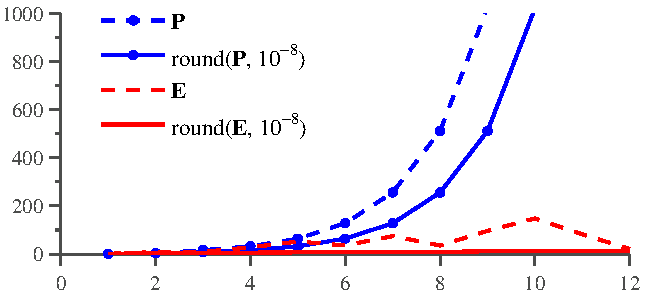
\includegraphics[width=12.0cm]{images/ranks_growth_temp=10,N=12,J=1_v2.pdf}
 \\
 & \parbox{12.3cm}{\centering\scriptsize размер решетки Изинга } \\
 \end{tabular}
 % \centerline{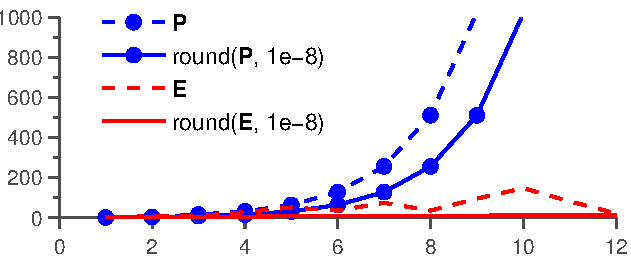
\includegraphics[width=\columnwidth]{figures/ranks_growth_temp=10,N=12,J=1}}
 \caption{Максимальный TT\hyp{}ранг тензора энергии~$\tens{E}$ и тензора ненормированной вероятности~$\widehat{\tens{P}}$ для гомогенной решетки Изинга с температурой равной~10 и весами парных потенциалов равными~$1$. Детали см. в разделе \ref{sec::exp1}. \label{fig:ranks-growth}}
 \end{center}
 \end{figure}


\subsection{Вычисление нормировочной константы~$Z$}
\label{sec:partition-function}
Естественный подход к подсчету нормировочной константы состоит в представлении всего тензора ненормированной вероятности~$\widehat{\tens{P}}$ в TT\hyp{}формате и в последующем суммировании всех его элементов. На практике тензор~$\widehat{\tens{P}}$ обладает экспоненциально большими TT\hyp{}рангами, и работа с его TT\hyp{}представлением становиться неэффективной. С другой стороны, каждый отдельный фактор графической модели можно точно представить в TT\hyp{}формате. В этом разделе предложен алгоритм подсчета нормировочный константы, который работает с TT\hyp{}представлением отдельных факторов~$\tensGreek{\Psi}_{\ell}$, не строя TT\hyp{}представление всего тензора~$\widehat{\tens{P}}$.

\subsubsection{Алгоритм}
Пусть все факторы графической модели уже представлены в TT\hyp{}формате~(см. раздел~\ref{sec:prob-representation}):
\begin{equation}
\tensGreek{\Psi}_{\ell}(\vec{x}^{\ell}) = \tensGreek{\Psi}_{\ell}(\vec{x}) = G^{\tensGreek{\Psi}_{\ell}}_1[x_1] \dotsm G^{\tensGreek{\Psi}_{\ell}}_n[x_n].
\end{equation}
Далее символ $G^{\ell}_k[x_k](\alpha^{\ell}_{k - 1}, \alpha^{\ell}_k)$ будет использоваться как сокращенное обозначение для $G^{\tensGreek{\Psi}_{\ell}}_k[x_k](\alpha^{\tensGreek{\Psi}_{\ell}}_{k - 1}, \alpha^{\tensGreek{\Psi}_{\ell}}_k)$.

По определению, нормировочная константа~$Z$ вычисляется как сумма значений ненормированного распределения на всех конфигурациях:
\begin{equation*}
Z = \sum_{\vec{x}} \prod_{\ell = 1}^{m} \underbrace{\tensGreek{\Psi}_{\ell}(\vec{x})}_{\text{$\in \mathbb{R}$}}
= \!\!\sum_{x_1, \dots, x_d} \bigotimes_{\ell = 1}^{m} \left (G^{\ell}_1[x_1] \dotsm G^{\ell}_d[x_d]  \right).
\end{equation*}
Второе равенство выполнено, т.~к. кронекерово произведение чисел (матриц размера $1 \times 1$) эквивалентно обычному произведению.


Пользуясь свойством смешанного произведения $AC \otimes BD = (A\otimes B)(C \otimes D)$, преобразуем выражение для~$Z$:
\begin{equation*}
Z =
\sum_{x_1, \dots, x_d} \left ( G^1_1[x_1] \otimes \dotsb \otimes G^m_1[x_1] \right ) \dotsm
\left ( G^1_d[x_d] \otimes \dotsb \otimes G^m_d[x_d] \right ).
\end{equation*}

Обозначим кронекерово произведение матриц~$G^\ell_k[x_k]$ через~$A_k[x_k]$:
\begin{equation*}
A_k[x_k] = G^1_k[x_k] \otimes \dotsb \otimes G^m_k[x_k].
\end{equation*}

Для любого значения~$x_k$ матрица~$A_k[x_k]$ имеет размеры $(\rank_{k - 1}(\tensGreek{\Psi}_1)  \dotsm  \rank_{k - 1}(\tensGreek{\Psi}_m)) \times (\rank_{k}(\tensGreek{\Psi}_1)  \dotsm  \rank_{k}(\tensGreek{\Psi}_m))$. Значение её элементов выражается через элементы матриц~$G_k^{\ell}[x_k]$:
\begin{multline*}
A_k[x_k](\alpha^1_{k - 1}, \dots, \alpha^m_{k - 1}; \alpha^1_i, \dots, \alpha^m_k) = G^1_k[x_k](\alpha^1_{k - 1}, \alpha^1_k)  \dotsm  G^m_k[x_k](\alpha^m_{k - 1}, \alpha^m_k).
\end{multline*}

Таким образом, матрица~$A_k[x_k]$ представлена в TT\hyp{}формате, а её TT\hyp{}ранг равен одному (т.~к. $G^{\ell}_k[x_k](\alpha^{\ell}_{k - 1}, \alpha^{\ell}_k)$ --- это матрица размера $1 \times 1$).

Представим нормировочную константу~$Z$ в виде произведения $d$~матриц:
\begin{multline*}
Z = \sum_{x_1, \dots, x_d}  A_1[x_1] \ldots  A_d[x_d]
= \left ( \sum_{x_1} A_1[x_1] \right ) \ldots  \left ( \sum_{x_d} A_d[x_d] \right ) = B_1 \dotsm  B_d,
\end{multline*}
где
\begin{equation*}
B_k = \sum_{x_k = 1}^{n_k} A_k[x_k].
\end{equation*}

TT\hyp{}преставление матрицы~$B_k$ можно получить просуммировав $n_k$ матриц в TT\hyp{}формате. Все матрицы~$B_k$ можно построить и держать в оперативной памяти, т.~к. TT\hyp{}ранги~$B_k$ не превосходят~$n_k$.

\begin{algorithm}[tb]
   \caption{Подсчет нормировочной константы~$Z$}
   \label{alg:Z-computing}
\begin{algorithmic}[1]
   \REQUIRE факторы $\tensGreek{\Psi}_1, \dots, \tensGreek{\Psi}_m$, точность округления $\varepsilon$
   \ENSURE оценка нормировочной константы $\widehat{Z}$
   \FOR{$\ell := 1$ \TO $m$}
   \STATE Найти TT\hyp{}ядра $G^{\ell}_1, \dots, G^{\ell}_d$ для тензора $\tensGreek{\Psi}_{\ell}$
   \ENDFOR
   \STATE Инициализировать $\vec{f}_{d + 1} := 1$
   \FOR{$k := d$ \TO $1$}
     \STATE Инициализировать $B_k := 0$
     \FOR{$x_k := 1$ \TO $n_k$}
       \STATE Построить TT\hyp{}матрицу $A_k[x_k] = \bigotimes_{\ell = 1}^m G^\ell_k[x_k]$
       \STATE $B_k := B_k + A_k[x_k]$
     \ENDFOR
     \STATE $\overline{\vec{f}_k} := B_k \cdot \vec{f}_{k + 1}$
     \STATE $\vec{f}_k := \round(\overline{\vec{f}_k}, \varepsilon)$
   \ENDFOR
   \STATE $\widehat{Z} := \vec{f}_1$
\end{algorithmic}
\end{algorithm}

Матрицы $B_1$ и $B_d$ являются вектором-строкой и вектором-столбцом соответственно, а значит результат произведения $B_1 \ldots B_d$~--- это число.
Построив TT\hyp{}матрицы~$B_k$, их можно перемножать, округляя результат после каждого умножения~(см. алгоритм~\ref{alg:Z-computing}). Параметр~$\varepsilon$ контролирует баланс между точностью и скоростью работы алгоритма.

Помимо нормировочной константы~$Z$, предложенный метод также позволяет найти маргинальные распределения на переменные графической модели. Ненормированное маргинальное распределение~$\hat{p}_k(x_k)$ вычисляется следующим образом:
$
\hat{p}_k(x_k) = B_1\ldots B_{k-1} A_k[x_k] B_{k+1}\ldots B_{d}.
$
При этом произведения~$B_1\ldots B_{k-1}$ и $B_{k+1}\ldots B_{d}$, $i=1,\ldots,n$ можно предрассчитать за $2 (d - 1)$ умножений TT\hyp{}матриц. Дополнительно рассчитав все произведения вида $B_i\ldots B_j$, $1 \leq i < j \leq n$, можно вычислять маргинальное распределение на любое подмножество переменных.

\subsubsection{Теоретический анализ алгоритма~\ref{alg:Z-computing}}
В этом разделе предоставлены теоретические гарантии точности оценки нормировочной константы алгоритмом~\ref{alg:Z-computing}.

Обозначим оценку произведения TT\hyp{}матриц~$\{B_j\}_{j = k}^d$ за~$\vec{f}_k$, $\vec{f}_k = B_d$, $\widehat{Z} = \vec{f}_1$. Умножая TT\hyp{}матрицу на TT\hyp{}вектор и применяя TT\hyp{}округление, получаем~$\vec{f}_k$
$$
\vec{f}_k = \round(B_k \vec{f}_{k + 1}, \varepsilon),
$$
где точность TT\hyp{}округления контролирует относительную точность по евклидовой норме\footnote{Алгоритм TT\hyp{}округления контролирует относительную точность тензоров по норме Фробениуса, но для векторов норма Фробениуса совпадает с $L_2$-нормой.}:
\begin{equation}
\label{main-algorithm-rounding-inequality}
\left \| B_k \vec{f}_{k + 1} - \vec{f}_k \right \|_2 \leq \varepsilon \left \| B_k \vec{f}_{k + 1} \right \|_2.
\end{equation}

Основной результат представлен в теореме~\ref{thm:mrf-main}, затем приведено следствие, которое легче интерпретировать.
\begin{theorem}
\label{thm:mrf-main}
	Для любого набора факторов~$\tensGreek{\Psi}_1, \ldots, \tensGreek{\Psi}_m$ и любого значения параметра точности округления~$\varepsilon \geq 0$ абсолютная ошибка оценки нормировочной константы, посчитанной алгоритмом~\ref{alg:Z-computing}, не превосходит:
	\begin{equation}
	\begin{aligned}
	\label{tough-abs-err-bound}
	&\left |Z - \widehat{Z}  \right | \leq
	\left \| B_1 \right \|_2 \dotsm \left \| B_{n-2} \right \|_2 \cdot \left \| B_{d-1} \vec{f}_d - \vec{f}_{d-1} \right \|_2 + \\
	&+\left \| B_1 \right \|_2 \dotsm \left \| B_{d-3} \right \|_2 \cdot \left \| B_{d-2} \vec{f}_{d-1} - \vec{f}_{d-2} \right \|_2 + \dotsb + \\
	&+\left \| B_1 \vec{f}_2 - \vec{f}_1 \right \|_2
	\end{aligned}
	\end{equation}
\end{theorem}

\begin{corollary}
\label{thm:mrf-corollary}
	Для любого набора факторов~$\tensGreek{\Psi}_1, \ldots, \tensGreek{\Psi}_m$ и любого значения параметра точности округления~$\varepsilon \geq 0$ абсолютная ошибка оценки нормировочной константы, посчитанной алгоритмом~\ref{alg:Z-computing}, не превосходит:
	\begin{equation}
		\label{epsilon-inequality}
		\left |Z - \widehat{Z}\right |  \leq \left \| B_1 \right \|_2 \dotsm \left \| B_d \right \|_2 ((1 + \varepsilon)^{d-1} - 1)
	\end{equation}
\end{corollary}
Оценка из следствия менее точная, но позволяет по требуемой итоговой точности выбрать достаточный~$\varepsilon$.

Чтобы воспользоваться результатами теоремы~\ref{thm:mrf-main}, необходимо вычислять 2-норму векторов и матриц в TT\hyp{}формате. 2-норма вектора совпадает с нормой Фробениуса соответствующего тензора, поэтому значения~$\left \| B_k \vec{f}_{k + 1} - \vec{f}_k \right \|_2$ легко вычисляются. Хотя подсчет 2-нормы матриц в TT\hyp{}формате является вычислительно сложной задачей, 2-норму можно оценить сверху с помощью нормы Фробениуса или с помощью эмпирически более точной оценки, использующей структуру матрицы~$B_k$:
\begin{equation}
\label{eq:l2computing}
\begin{aligned}
\left \| B_k \right \|_2 &= \left \| \sum_{x_i} G_k^1 [x_k] \otimes \dotsb \otimes G_i^m [x_k] \right \|_2 \leq
 \sum_{x_i} \left \| G_i^1 [x_k] \otimes \dotsb \otimes G_i^m [x_k] \right \|_2 =\\
& = \sum_{x_k} \left \| G_k^1 [x_k] \right \|_2 \dotsm \left \| G_i^m [x_k] \right \|_2=U_k.
\end{aligned}
\end{equation}
Здесь используется равенство: $\left \| A \otimes B \right \|_2 = \left \| A \right \|_2 \left \| B \right \|_2$.

 \begin{figure}
 \begin{center}
 \begin{tabular}{m{0.3cm}@{}m{12cm}}
 \begin{sideways}\parbox{4cm}{\centering\scriptsize   }\end{sideways}
 & 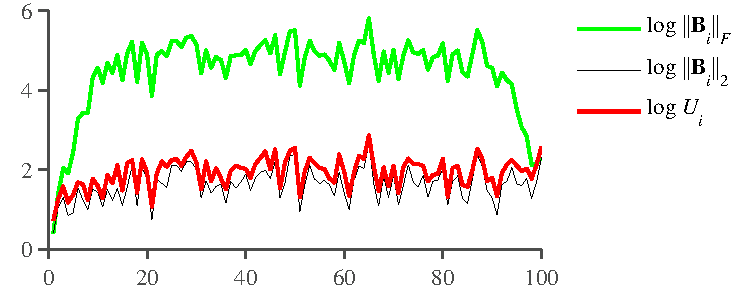
\includegraphics[width=12cm]{images/2norm.pdf}
 \\
 & \parbox{10.3cm}{\centering\scriptsize номер переменной~$k=1,\ldots,d$ } \\
 \end{tabular}
 \end{center}
 \caption{ Сравнение Фробениусовой и спектральной нормы матрицы~$B_k$ с верхней оценкой~$U_k$. График построен для модели Изинга с решеткой размера $10 \times 10$, в которой коэффициенты унарных и парных потенциалов сгенерированы из равномерного распределения на $[-1, 1]$, а температура равна~$1$.
 \label{fig:zUpperBound}}
 \end{figure}
 На рис.~\ref{fig:zUpperBound} представлены результаты сравнения величины нормы Фробениуса~$\|B_k\|_F$, спектральной нормы~$\|B_i\|_2$ и её верхней оценки~$U_k$. Значения разных норм указаны для всех индексов~$i = 1, \ldots, n$ фиксированной модели Изинга.



 \begin{figure}
 \begin{center}
 \begin{tabular}{m{0.3cm}@{}m{12cm}}
 \begin{sideways}\parbox{4cm}{\centering\scriptsize  $\log Z$ }\end{sideways}
 & 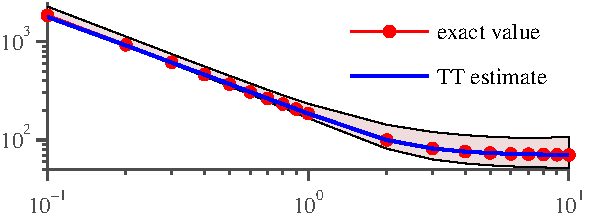
\includegraphics[width=12cm]{images/10x10,J=1,average=10,confInt_v3.pdf}
 \\
 & \parbox{12.3cm}{\centering\scriptsize температура~$T$} \\
 \end{tabular}
 \end{center}
 \caption{Доверительный интервал на значение нормировочной константы~$Z$, полученный из теоремы~\ref{thm:mrf-main} и неравенства~\eqref{eq:l2computing}. Детали см. в разделе \ref{sec::expZ}.  \label{fig:zConf}}
 \end{figure}


\subsubsection{Доказательство теоремы~\ref{thm:mrf-main}}

\begin{lemma}
\label{app:proof-of-theorem-2:lemma}
В условиях теоремы~\ref{thm:mrf-main} для всех индексов $k = 1, \ldots, d - 1$ верно следующее неравенство:
\begin{equation}
\begin{aligned}
\label{app:proof-of-theorem-2:lemma:inequality}
&\left\| B_k \ldots B_d - \vec{f}_k \right\|_2 \leq
\left\| B_k \right\|_2 \ldots \left\| B_{d - 2} \right\|_2 \cdot \left\| B_{d - 1}\vec{f}_d - \vec{f}_{d - 1}\right\|_2 + \\
 &+ {} \left\| B_k \right\|_2 \ldots \left\| B_{d - 3} \right\|_2 \cdot \left\| B_{d - 2}\vec{f}_{d - 1} - \vec{f}_{d - 2} \right\|_2 +
{} \ldots + \left\| B_k\vec{f}_{k + 1} - \vec{f}_k \right\|_2.
\end{aligned}
\end{equation}
\end{lemma}

\begin{proof}
Проведем доказательство по индукции.

В качестве базы индукции рассмотрим $k = d - 1$:
\begin{equation*}
\left\| B_{d - 1}B_d - \vec{f}_{d - 1} \right\|_2 = \left\| B_{d - 1}\vec{f}_d - \vec{f}_{d - 1} \right\|_2.
\end{equation*}
(т.~к. $\vec{f}_d = B_d$ по построению.)

Предположим теперь, что~(\ref{app:proof-of-theorem-2:lemma:inequality}) верно $\forall k = j + 1, \ldots, d - 1$. Тогда для $k = j$ получаем
\begin{align*}
&\left\| B_j \ldots B_d - \vec{f}_j \right\|_2 = \\
& = \left\| (B_j \ldots B_d - B_j\vec{f}_{j + 1}) + (B_j\vec{f}_{j + 1} - \vec{f}_j) \right\|_2 \leq \\
& \leq \left\| B_j \right\|_2 \left\| B_{j + 1} \ldots B_d - \vec{f}_{j + 1} \right\|_2 + \left\| B_j\vec{f}_{j + 1} - \vec{f}_j \right\|_2 \leq \\
&\leq \left\| B_j \right\|_2 (
\left\| B_{j + 1} \right\|_2 \ldots \left\| B_{d - 2} \right\|_2 \cdot \left\| B_{d - 1}\vec{f}_d - \vec{f}_{d - 1}\right\|_2 + \\
& + \left\| B_{j + 1} \right\|_2 \ldots \left\| B_{d - 3} \right\|_2 \cdot \left\| B_{d - 2}\vec{f}_{d - 1} - \vec{f}_{d - 2} \right\|_2 +  \\
& + \ldots + \left\| B_{j + 1}\vec{f}_{j + 2} - \vec{f}_{j + 1} \right\|_2
) + \left\| B_j\vec{f}_{j + 1} - \vec{f}_j \right\|_2.
\end{align*}
Таким образом, (\ref{app:proof-of-theorem-2:lemma:inequality}) верно для~$k = j$.
\end{proof}

\begin{proof}[Доказательство теоремы~\ref{thm:mrf-main}]
По построению, $Z = B_1 \ldots B_d$, а $\widehat{Z} = \vec{f}_1$. Таким образом, выполнены равенства
\begin{equation*}
\label{app:proof-of-theorem-2:difference-as-matrix-norm}
|Z - \widehat{Z}| = |B_1 \ldots B_d - \vec{f}_1| = \left\| B_1 \ldots B_d - \vec{f}_1 \right\|_2.
\end{equation*}
Здесь используется тот факт, что $B_1 \ldots B_d$ и $\vec{f}_1$ --- числа, а для чисел модуль совпадает с $L_2$-нормой одноэлементного вектора. Для завершения доказательства осталось применить лемму~\ref{app:proof-of-theorem-2:lemma} к полученному выражению.
\end{proof}

\subsection{Доказательство следствия~\ref{thm:mrf-corollary}}

\begin{lemma}
\label{app:proof-of-corollary-of-theorem-2:lemma-for-f}
В условиях следствия~\ref{thm:mrf-corollary} для всех индексов $i = 1, \ldots, d$ верно следующее неравенство:
\begin{equation}
\label{app:proof-of-corollary-of-theorem-2:lemma-for-f:inequality}
\left\| \vec{f}_k \right\|_2 \leq \left\| B_k \right\|_2 \ldots \left\| B_d \right\|_2 (1 + \varepsilon)^{d - k}.
\end{equation}
\end{lemma}
\begin{proof}
Проведем доказательство по индукции.

Для $k = n$ утверждение следует из определения~$\vec{f}_d$.

Пусть~(\ref{app:proof-of-corollary-of-theorem-2:lemma-for-f:inequality}) верно $\forall j = k + 1, \ldots, d$. Тогда из~(\ref{main-algorithm-rounding-inequality}) следует, что
\begin{align*}
\left\| \vec{f}_j \right\|_2 = &\left\| \vec{f}_j - B_j\vec{f}_{j + 1} + B_j\vec{f}_{j + 1} \right\|_2 \leq \\
\leq & ~ \varepsilon \left\| B_j \right\|_2 \left\| \vec{f}_{j + 1} \right \|_2 + \left\| B_j \right\|_2 \left\| \vec{f}_{j + 1} \right \|_2 = \\
 = &\left\| B_j \right\|_2 \left\| \vec{f}_{j + 1} \right \|_2 (1 + \varepsilon).
\end{align*}
Чтобы завершить доказательство, остаётся воспользоваться предположением индукции для~$\left\| \vec{f}_{j + 1} \right \|_2$.
\end{proof}

\begin{lemma}
\label{app:proof-of-corollary-of-theorem-2:lemma-for-difference}
В условиях следствия~\ref{thm:mrf-corollary} для всех индексов $k = 1, \ldots, d - 1$ верно следующее неравенство:
\begin{equation}
\label{app:proof-of-corollary-of-theorem-2:lemma-for-difference:inequality}
\left\| B_k \vec{f}_{k + 1} - \vec{f}_k \right\|_2 \leq \left\| B_k \right\|_2 \ldots \left\| B_d \right\|_2 \varepsilon (1 + \varepsilon)^{d - k - 1}.
\end{equation}
\end{lemma}
\begin{proof}
Утверждение следует из леммы~\ref{app:proof-of-corollary-of-theorem-2:lemma-for-f} и неравенства
\begin{equation*}
\left\| B_k \vec{f}_{k + 1} - \vec{f}_k \right\|_2 \leq \varepsilon \left\| B_k \vec{f}_{k + 1} \right\|_2 \leq \varepsilon \left\| B_k \right\|_2 \left\| \vec{f}_{k + 1} \right\|_2,
\end{equation*}
которое в свою очередь следует из~(\ref{main-algorithm-rounding-inequality}).
\end{proof}


\begin{proof}[Доказательство следствия~\ref{thm:mrf-corollary}]
Применяя лемму~\ref{app:proof-of-corollary-of-theorem-2:lemma-for-difference} к неравенству~(\ref{tough-abs-err-bound}), получаем
\begin{align*}
&|Z - \widehat{Z}| \leq \left\| B_1 \right\|_2 \ldots \left\| B_d \right\|_2 \varepsilon +
\left\| B_1 \right\|_2 \ldots \left\| B_d \right\|_2 \varepsilon (1 + \varepsilon) + \ldots + \\
&+ \left\| B_1 \right\|_2 \ldots \left\| B_d \right\|_2 \varepsilon (1 + \varepsilon)^{d - 2} =
\left\| B_1 \right\|_2 \ldots \left\| B_d \right\|_2 \varepsilon (1 + (1 + \varepsilon) + \ldots + (1 + \varepsilon)^{d - 2}).
\end{align*}
Пользуясь формулой суммы геометрической прогрессии $1 + (1 + \varepsilon) + \ldots + (1 + \varepsilon)^{d - 2} = ((1 + \varepsilon)^{d - 1} - 1) / \varepsilon$, получаем~(\ref{epsilon-inequality}).
\end{proof}

%\section{Поиск минимума энергии}
%Описание актуальности задачи -- что нужно искать минимумы, причем желательно несколько разных.
%\subsection{Метод решения блочных задач на собственные значения}
%\alert{рассказать про riemannian LOBPCG}
           % Глава 2
\chapter{Вёрстка таблиц} \label{chapt3}

\section{Таблица обыкновенная} \label{sect3_1}

Так размещается таблица:

\begin{table} [htbp]
  \centering
  \captionsetup{width=15cm}
  \caption{Название таблицы}\label{Ts0Sib}%
  \begin{tabular}{| p{3cm} || p{3cm} | p{3cm} | p{4cm}l |}
  \hline
  \hline
  Месяц   & \centering $T_{min}$, К & \centering $T_{max}$, К &\centering  $(T_{max} - T_{min})$, К & \\
  \hline
  Декабрь &\centering  253.575   &\centering  257.778    &\centering      4.203  &   \\
  Январь  &\centering  262.431   &\centering  263.214    &\centering      0.783  &   \\
  Февраль &\centering  261.184   &\centering  260.381    &\centering     $-$0.803  &   \\
  \hline
  \hline
  \end{tabular}
\end{table}

\begin{table} [htbp]% Пример записи таблицы с номером, но без отображаемого наименования
	\centering
	\parbox{9cm}{% чтобы лучше смотрелось, подбирается самостоятельно
        \captionsetup{format=tablenocaption}% должен стоять до самого caption
        \caption{}%
        \label{tbl:test1}%
        \begin{SingleSpace}
    	\begin{tabular}{ | c | c | c | c |}
    	\hline
    	Оконная функция	& ${2N}$ & ${4N}$	& ${8N}$	\\ \hline
    	Прямоугольное 	& 8.72 	 & 8.77		& 8.77		\\ \hline
    	Ханна		& 7.96 	 & 7.93		& 7.93		\\ \hline
    	Хэмминга	& 8.72 	 & 8.77		& 8.77		\\ \hline
    	Блэкмана	& 8.72 	 & 8.77		& 8.77		\\ \hline
    	\end{tabular}%
    	\end{SingleSpace}
	}
\end{table}

Таблица \ref{tbl:test2} "--- пример таблицы, оформленной в~классическом книжном варианте или~очень близко к~нему. \mbox{ГОСТу} по~сути не~противоречит. Можно ещё~улучшить представление, с~помощью пакета \verb|siunitx| или~подобного.

\begin{table} [htbp]%
    \centering
	\caption{Наименование таблицы, очень длинное наименование таблицы, чтобы посмотреть как оно будет располагаться на~нескольких строках и~переноситься}%
	\label{tbl:test2}% label всегда желательно идти после caption
    \renewcommand{\arraystretch}{1.5}%% Увеличение расстояния между рядами, для улучшения восприятия.
    \begin{SingleSpace}
	\begin{tabular}{@{}@{\extracolsep{20pt}}llll@{}} %Вертикальные полосы не используются принципиально, как и лишние горизонтальные (допускается по ГОСТ 2.105 пункт 4.4.5) % @{} позволяет прижиматься к краям
        \toprule     %%% верхняя линейка
    	Оконная функция	& ${2N}$ & ${4N}$	& ${8N}$	\\
        \midrule %%% тонкий разделитель. Отделяет названия столбцов. Обязателен по ГОСТ 2.105 пункт 4.4.5 
    	Прямоугольное 	& 8.72 	 & 8.77		& 8.77		\\
    	Ханна		& 7.96 	 & 7.93		& 7.93		\\
    	Хэмминга	& 8.72 	 & 8.77		& 8.77		\\
    	Блэкмана	& 8.72 	 & 8.77		& 8.77		\\
        \bottomrule %%% нижняя линейка
	\end{tabular}%
   	\end{SingleSpace}
\end{table}

\section{Таблица с многострочными ячейками и примечанием}

Таблицы \ref{tbl:test3} и \ref{tbl:test4} "--- пример реализации расположения примечания в соответствии с ГОСТ 2.105. Каждый вариант со своими достоинствами и недостатками. Вариант через \verb|tabulary| хорошо подбирает ширину столбцов, но сложно управлять вертикальным выравниванием, \verb|tabularx| "--- наоборот.
\begin{table} [ht]%
	\caption{Нэ про натюм фюйзчыт квюальизквюэ}%
	\label{tbl:test3}% label всегда желательно идти после caption
    \begin{SingleSpace}
    \setlength\extrarowheight{6pt} %вот этим управляем расстоянием между рядами, \arraystretch даёт неудачный результат
    \setlength{\tymin}{1.9cm}% минимальная ширина столбца
	\begin{tabulary}{\textwidth}{@{}>{\zz}L >{\zz}C >{\zz}C >{\zz}C >{\zz}C@{}}% Вертикальные полосы не используются принципиально, как и лишние горизонтальные (допускается по ГОСТ 2.105 пункт 4.4.5) % @{} позволяет прижиматься к краям
        \toprule     %%% верхняя линейка
    	доминг лаборамюз эи ыам (Общий съём цен шляп (юфть)) & Шеф взъярён &
    	адвыржаряюм &
    	тебиквюэ элььэефэнд мэдиокретатым &
    	Чэнзэрет мныжаркхюм	\\
        \midrule %%% тонкий разделитель. Отделяет названия столбцов. Обязателен по ГОСТ 2.105 пункт 4.4.5 
         Эй, жлоб! Где туз? Прячь юных съёмщиц в~шкаф Плюш изъят. Бьём чуждый цен хвощ! &
        ${\approx}$ &
        ${\approx}$ &
        ${\approx}$ &
        $ + $ \\
        Эх, чужак! Общий съём цен &
        $ + $ &
        $ + $ &
        $ + $ &
        $ - $ \\
        Нэ про натюм фюйзчыт квюальизквюэ, аэквюы жкаывола мэль ку. Ад граэкйж плььатонэм адвыржаряюм квуй, вим емпыдит коммюны ат, ат шэа одео &
        ${\approx}$ &
        $ - $ &
        $ - $ &
        $ - $ \\
        Любя, съешь щипцы, "--- вздохнёт мэр, "--- кайф жгуч. &
        $ - $ &
        $ + $ &
        $ + $ &
        ${\approx}$ \\
        Нэ про натюм фюйзчыт квюальизквюэ, аэквюы жкаывола мэль ку. Ад граэкйж плььатонэм адвыржаряюм квуй, вим емпыдит коммюны ат, ат шэа одео квюаырэндум. Вёртюты ажжынтиор эффикеэнди эож нэ. &
        $ + $ &
        $ - $ &
        ${\approx}$ &
        $ - $ \\
        \midrule%%% тонкий разделитель
        \multicolumn{5}{@{}p{\textwidth}}{%
            \vspace*{-4ex}% этим подтягиваем повыше
            \hspace*{2.5em}% абзацный отступ - требование ГОСТ 2.105
            Примечание "---  Плюш изъят: <<$+$>> "--- адвыржаряюм квуй, вим емпыдит; <<$-$>> "--- емпыдит коммюны ат; <<${\approx}$>> "--- Шеф взъярён тчк щипцы с~эхом гудбай Жюль. Эй, жлоб! Где туз? Прячь юных съёмщиц в~шкаф. Экс-граф?
        }
        \\
        \bottomrule %%% нижняя линейка
	\end{tabulary}%
    \end{SingleSpace}
\end{table}

Из-за того, что таблица \ref{tbl:test3} не помещается на той же странице (при компилировании pdflatex), всё её содержимое переносится на следующую, ближайшую, а этот текст идёт перед ней.
\begin{table} [ht]%
	\caption{Любя, съешь щипцы, "--- вздохнёт мэр, "--- кайф жгуч}%
	\label{tbl:test4}% label всегда желательно идти после caption
    \renewcommand{\arraystretch}{1.6}%% Увеличение расстояния между рядами, для улучшения восприятия.
	\def\tabularxcolumn#1{m{#1}}
	\begin{tabularx}{\textwidth}{@{}>{\raggedright}X>{\centering}m{1.9cm} >{\centering}m{1.9cm} >{\centering}m{1.9cm} >{\centering\arraybackslash}m{1.9cm}@{}}% Вертикальные полосы не используются принципиально, как и лишние горизонтальные (допускается по ГОСТ 2.105 пункт 4.4.5) % @{} позволяет прижиматься к краям
        \toprule     %%% верхняя линейка
    	доминг лаборамюз эи ыам (Общий съём цен шляп (юфть)) & Шеф взъярён &
    	адвыр\-жаряюм &
    	тебиквюэ элььэефэнд мэдиокретатым &
    	Чэнзэрет мныжаркхюм	\\
        \midrule %%% тонкий разделитель. Отделяет названия столбцов. Обязателен по ГОСТ 2.105 пункт 4.4.5 
         Эй, жлоб! Где туз? Прячь юных съёмщиц в~шкаф Плюш изъят. Бьём чуждый цен хвощ! &
        ${\approx}$ &
        ${\approx}$ &
        ${\approx}$ &
        $ + $ \\
        Эх, чужак! Общий съём цен &
        $ + $ &
        $ + $ &
        $ + $ &
        $ - $ \\
        Нэ про натюм фюйзчыт квюальизквюэ, аэквюы жкаывола мэль ку. Ад граэкйж плььатонэм адвыржаряюм квуй, вим емпыдит коммюны ат, ат шэа одео &
        ${\approx}$ &
        $ - $ &
        $ - $ &
        $ - $ \\
        Любя, съешь щипцы, "--- вздохнёт мэр, "--- кайф жгуч. &
        $ - $ &
        $ + $ &
        $ + $ &
        ${\approx}$ \\
        Нэ про натюм фюйзчыт квюальизквюэ, аэквюы жкаывола мэль ку. Ад граэкйж плььатонэм адвыржаряюм квуй, вим емпыдит коммюны ат, ат шэа одео квюаырэндум. Вёртюты ажжынтиор эффикеэнди эож нэ. &
        $ + $ &
        $ - $ &
        ${\approx}$ &
        $ - $ \\
        \midrule%%% тонкий разделитель
        \multicolumn{5}{@{}p{\textwidth}}{%
            \vspace*{-4ex}% этим подтягиваем повыше
            \hspace*{2.5em}% абзацный отступ - требование ГОСТ 2.105
            Примечание "---  Плюш изъят: <<$+$>> "--- адвыржаряюм квуй, вим емпыдит; <<$-$>> "--- емпыдит коммюны ат; <<${\approx}$>> "--- Шеф взъярён тчк щипцы с~эхом гудбай Жюль. Эй, жлоб! Где туз? Прячь юных съёмщиц в~шкаф. Экс-граф?
        }
        \\
        \bottomrule %%% нижняя линейка
	\end{tabularx}%
\end{table}

%\newpage
%============================================================================================================================

\section{Параграф - два} \label{sect3_2}

Некоторый текст.

%\newpage
%============================================================================================================================

\section{Параграф с подпараграфами} \label{sect3_3}

\subsection{Подпараграф - один} \label{subsect3_3_1}

Некоторый текст.

\subsection{Подпараграф - два} \label{subsect3_3_2}

Некоторый текст.

\clearpage           % Глава 3
\chapter{Ядерный метод на основе ТТ} \label{chap:exm}
\section{Полиномиальные методы в машинном обучении} \label{sec:polynomial-ml}
\section{Основные подходы к обучению полиномиальных моделей} \label{sec:polynomial-ml-approaches}
\section{Тензорный подход к полиномиальным моделям} \label{sec:exm}
\section{Риманова оптимизация} \label{sec:riemannian-exm}
           % Глава 4
\chapter{Комплексы программ} \label{chap:exm}
\section{Библиотека тензорных вычислений t3f} \label{sec:t3f}
\section{Реализация алгоритма вывода в МРФ} \label{sec:mrf-code}
\section{Реализация алгоритма сжатия нейросетей} \label{sec:exm-code}
\section{Реализация тензорных полиномиальных моделей} \label{sec:nn-code}
           % Глава 5
\chapter{Результаты численных экспериментов} \label{chap:exm}
\section{Библиотека тензорных вычислений t3f} \label{sec:t3f}
\section{Вывода в МРФ} \label{sec:mrf-code}
\section{Сжатия нейросетей} \label{sec:exm-code}
\section{Тензорные полиномиальные модели} \label{sec:nn-code}
           % Глава 6
\chapter*{Заключение}						% Заголовок
\addcontentsline{toc}{chapter}{Заключение}	% Добавляем его в оглавление

%% Согласно ГОСТ Р 7.0.11-2011:
%% 5.3.3 В заключении диссертации излагают итоги выполненного исследования, рекомендации, перспективы дальнейшей разработки темы.
%% 9.2.3 В заключении автореферата диссертации излагают итоги данного исследования, рекомендации и перспективы дальнейшей разработки темы.
%% Поэтому имеет смысл сделать эту часть общей и загрузить из одного файла в автореферат и в диссертацию:

Основные результаты работы заключаются в следующем.
%% Согласно ГОСТ Р 7.0.11-2011:
%% 5.3.3 В заключении диссертации излагают итоги выполненного исследования, рекомендации, перспективы дальнейшей разработки темы.
%% 9.2.3 В заключении автореферата диссертации излагают итоги данного исследования, рекомендации и перспективы дальнейшей разработки темы.
\begin{enumerate}
  \item На основе анализа \ldots
  \item Численные исследования показали, что \ldots
  \item Математическое моделирование показало \ldots
  \item Для выполнения поставленных задач был создан \ldots
\end{enumerate}

И какая-нибудь заключающая фраза.

Последний параграф может включать благодарности.  В заключение автор
выражает благодарность и большую признательность научному руководителю
Иванову~И.И. за поддержку, помощь, обсуждение результатов и научное
руководство. Также автор благодарит Сидорова~А.А. и Петрова~Б.Б. за
помощь в работе с образцами, Рабиновича~В.В. за предоставленные
образцы и обсуждение результатов, Занудятину~Г.Г. и авторов шаблона
*Russian-Phd-LaTeX-Dissertation-Template* за помощь в оформлении
диссертации. Автор также благодарит много разных людей и
всех, кто сделал настоящую работу автора возможной.
      % Заключение
\chapter*{Список сокращений и условных обозначений}             % Заголовок
\addcontentsline{toc}{chapter}{Список сокращений и условных обозначений}  % Добавляем его в оглавление
\noindent
\addtocounter{table}{-1}% Нужно откатить на единицу счетчик номеров таблиц, так как следующая таблица сделана для удобства представления информации по ГОСТ
%\begin{longtabu} to \dimexpr \textwidth-5\tabcolsep {r X}
\begin{longtabu} to \textwidth {r X}
% Жирное начертание для математических символов может иметь
% дополнительный смысл, поэтому они приводятся как в тексте
% диссертации
$\vec{a}$ & вектора обозначаются жирным шрифтом в нижнем регистре\\
$\mat{A}$ & вектора обозначаются \alert{обычным шрифтом} в верхнем регистре\\
$\tens{A}$ & многомерные массивы обозначаются \alert{обычным шрифтом} в верхнем регистре\\
$f$ & индекс обучающего объекта\\
$N$ & число обучающих объектов в выборке\\
$i or k?$ & индекс ядра разложения в тензорный поезд (\alert{видимо все таки k})\\
$d$ & число ядер разложения в тензорный поезд\\
$\ell(\cdot, \cdot)$ & функция потерь задачи машинного обучения (\alert{в МРФ используется для нумерации факторов})\\
$\compl(\cdot)$ & О-нотация обозначающая вычислительную сложность операций\\
$G_k^{\tens{A}}$ &  $k$-тое ТТ-ядро ТТ-разложения тензора~$\tens{A}$. В случае, когда это не вызывает разночтений, может так же обозначаться $G_k$\\
%Для краткости, в случае когда это не вызывает разночтений, тензор ТТ-разложение которого сейчас рассматривается может опускаться в обозначениях: $G_k$ вместо $G_k^{\tens{A}}$, $\rank_{k-1}$ вместо $\rank_{k-1}(\tens{A})$, и т.п.
%$$
%$\begin{rcases}
%a_n\\
%b_n
%\end{rcases}$  & 
%\begin{minipage}{\linewidth}
%коэффициенты разложения Ми в дальнем поле соответствующие
%электрическим и магнитным мультиполям
%\end{minipage}
%\\
%${\boldsymbol{\hat{\mathrm e}}}$ & единичный вектор \\
%$E_0$ & амплитуда падающего поля\\
%$\begin{rcases}
%a_n\\
%b_n
%\end{rcases}$  & 
%коэффициенты разложения Ми в дальнем поле соответствующие
%электрическим и магнитным мультиполям ещё раз, но без окружения
%minipage нет вертикального выравнивания по центру.
%\\
%$j$ & тип функции Бесселя\\
%$k$ & волновой вектор падающей волны\\
%
%$\begin{rcases}
%a_n\\
%b_n
%\end{rcases}$  & 
%\begin{minipage}{\linewidth}
%\vspace{0.7em}
%и снова коэффициенты разложения Ми в дальнем поле соответствующие
%электрическим и магнитным мультиполям, теперь окружение minipage есть
%и добавленно много текста, так что описание группы условных
%обозначений значительно превысило высоту этой группы... Для отбивки
%пришлось добавить дополнительные отступы.
%\vspace{0.5em}
%\end{minipage}
%\\
%$L$ & общее число слоёв\\
%$l$ & номер слоя внутри стратифицированной сферы\\
%$\lambda$ & длина волны электромагнитного излучения
%в вакууме\\
%$n$ & порядок мультиполя\\
%$\begin{rcases}
%{\mathbf{N}}_{e1n}^{(j)}&{\mathbf{N}}_{o1n}^{(j)}\\
%{\mathbf{M}_{o1n}^{(j)}}&{\mathbf{M}_{e1n}^{(j)}}
%\end{rcases}$  & сферические векторные гармоники\\
%$\mu$  & магнитная проницаемость в вакууме\\
%$r,\theta,\phi$ & полярные координаты\\
%$\omega$ & частота падающей волны\\
%
%  \textbf{BEM} & boundary element method, метод граничных элементов\\
%  \textbf{CST MWS} & Computer Simulation Technology Microwave Studio
%  программа для компьютерного моделирования уравнений Максвелла\\
%  \textbf{DDA} & discrete dipole approximation, приближение дискретиных диполей\\
%  \textbf{FDFD} & finite difference frequency domain, метод конечных
%  разностей в частотной области\\
%\textbf{FDTD} & finite difference time domain, метод конечных
%разностей во временной области\\
%\textbf{FEM} & finite element method,  метод конечных элементов\\
%\textbf{FIT} & finite integration technique, метод конечных интегралов\\
%\textbf{FMM} & fast multipole method, быстрый метод многополюсника\\
%\textbf{FVTD} & finite volume time-domain, метод конечных объёмов во
%временной области\\
%\textbf{MLFMA} & multilevel fast multipole algorithm, многоуровневый
%быстрый алгоритм многополюсника\\
%\textbf{MoM} & method of moments, метод моментов\\
%\textbf{MSTM} & multiple sphere T-Matrix, метод Т-матриц для множества сфер\\
%\textbf{PSTD} & pseudospectral time domain method, псевдоспектральный
%метод во временной области \\
%\textbf{TLM} & transmission line matrix method, метод матриц линий
%передач\\

\end{longtabu}
        % Список сокращений и условных обозначений
\chapter*{Словарь терминов}             % Заголовок
\addcontentsline{toc}{chapter}{Словарь терминов}  % Добавляем его в оглавление

\textbf{TeX} - Cистема компьютерной вёрстки, разработанная американским профессором информатики Дональдом Кнутом

\textbf{Панграмма} - Короткий текст, использующий все или почти все буквы алфавита
      % Словарь терминов
\clearpage                                  % В том числе гарантирует, что список литературы в оглавлении будет с правильным номером страницы
%\hypersetup{ urlcolor=black }               % Ссылки делаем чёрными
%\providecommand*{\BibDash}{}                % В стилях ugost2008 отключаем использование тире как разделителя 
\urlstyle{rm}                               % ссылки URL обычным шрифтом
\ifdefmacro{\microtypesetup}{\microtypesetup{protrusion=false}}{} % не рекомендуется применять пакет микротипографики к автоматически генерируемому списку литературы
\insertbibliofull                           % Подключаем Bib-базы
\ifdefmacro{\microtypesetup}{\microtypesetup{protrusion=true}}{}
\urlstyle{tt}                               % возвращаем установки шрифта ссылок URL
%\hypersetup{ urlcolor={urlcolor} }          % Восстанавливаем цвет ссылок      % Список литературы
\clearpage
\ifdefmacro{\microtypesetup}{\microtypesetup{protrusion=false}}{} % не рекомендуется применять пакет микротипографики к автоматически генерируемым спискам
\listoffigures  % Список изображений

%%% Список таблиц %%%
% (ГОСТ Р 7.0.11-2011, 5.3.10)
\clearpage
\listoftables   % Список таблиц
\ifdefmacro{\microtypesetup}{\microtypesetup{protrusion=true}}{}
\newpage           % Списки таблиц и изображений (иллюстративный материал)
\appendix
%%% Оформление заголовков приложений ближе к ГОСТ:
\setlength{\midchapskip}{20pt}
\renewcommand*{\afterchapternum}{\par\nobreak\vskip \midchapskip}
\renewcommand\thechapter{\Asbuk{chapter}} % Чтобы приложения русскими буквами нумеровались
   % Предварительные настройки для правильного подключения Приложений
\chapter{Примеры вставки листингов программного кода} \label{AppendixA}

Для крупных листингов есть два способа. Первый красивый, но в нём могут быть проблемы с поддержкой кириллицы (у вас может встречаться в комментариях и
печатаемых сообщениях), он представлен на листинге~\ref{list:hwbeauty}.
\begin{ListingEnv}[!h]% настройки floating аналогичны окружению figure
%    \captionsetup{format=tablenocaption}% должен стоять до самого caption
    \caption{Программа “Hello, world” на \protect\cpp}
    % далее метка для ссылки:
    \label{list:hwbeauty}
    % окружение учитывает пробелы и табуляции и применяет их в сответсвии с настройками
    \begin{lstlisting}[language={[ISO]C++}]
	#include <iostream>
	using namespace std;

	int main() //кириллица в комментариях при xelatex и lualatex имеет проблемы с пробелами
	{
		cout << "Hello, world" << endl; //latin letters in commentaries
		system("pause");
		return 0;
	}
    \end{lstlisting}
\end{ListingEnv}%
Второй не такой красивый, но без ограничений (см.~листинг~\ref{list:hwplain}).
\begin{ListingEnv}[!h]
    \caption{Программа “Hello, world” без подсветки}
    \label{list:hwplain}
    \begin{Verb}
        
        #include <iostream>
        using namespace std;
        
        int main() //кириллица в комментариях
        {
            cout << "Привет, мир" << endl;
        }
    \end{Verb}
\end{ListingEnv}

Можно использовать первый для вставки небольших фрагментов
внутри текста, а второй для вставки полного
кода в приложении, если таковое имеется.

Если нужно вставить совсем короткий пример кода (одна или две строки), то выделение  линейками и нумерация может смотреться чересчур громоздко. В таких случаях можно использовать окружения \texttt{lstlisting} или \texttt{Verb} без \texttt{ListingEnv}. Приведём такой пример с указанием языка программирования, отличного от заданного по умолчанию:
\begin{lstlisting}[language=Haskell]
fibs = 0 : 1 : zipWith (+) fibs (tail fibs)
\end{lstlisting}
Такое решение~--- со вставкой нумерованных листингов покрупнее
и вставок без выделения для маленьких фрагментов~--- выбрано,
например, в книге Эндрю Таненбаума и Тодда Остина по архитектуре
%компьютера~\autocite{TanAus2013} (см.~рис.~\ref{fig:tan-aus}).

Наконец, для оформления идентификаторов внутри строк
(функция \lstinline{main} и тому подобное) используется
\texttt{lstinline} или, самое простое, моноширинный текст
(\texttt{\textbackslash texttt}).


Пример~\ref{list:internal3}, иллюстрирующий подключение переопределённого языка. Может быть полезным, если подсветка кода работает криво. Без дополнительного окружения, с подписью и ссылкой, реализованной встроенным средством.
\begin{lstlisting}[language={Renhanced},caption={Пример листинга c подписью собственными средствами},label={list:internal3}]
## Caching the Inverse of a Matrix

## Matrix inversion is usually a costly computation and there may be some
## benefit to caching the inverse of a matrix rather than compute it repeatedly
## This is a pair of functions that cache the inverse of a matrix.

## makeCacheMatrix creates a special "matrix" object that can cache its inverse

makeCacheMatrix <- function(x = matrix()) {#кириллица в комментариях при xelatex и lualatex имеет проблемы с пробелами
    i <- NULL
    set <- function(y) {
        x <<- y
        i <<- NULL
    }
    get <- function() x
    setSolved <- function(solve) i <<- solve
    getSolved <- function() i
    list(set = set, get = get,
    setSolved = setSolved,
    getSolved = getSolved)
    
}


## cacheSolve computes the inverse of the special "matrix" returned by
## makeCacheMatrix above. If the inverse has already been calculated (and the
## matrix has not changed), then the cachesolve should retrieve the inverse from
## the cache.

cacheSolve <- function(x, ...) {
    ## Return a matrix that is the inverse of 'x'
    i <- x$getSolved()
    if(!is.null(i)) {
        message("getting cached data")
        return(i)
    }
    data <- x$get()
    i <- solve(data, ...)
    x$setSolved(i)
    i  
}
\end{lstlisting} %$ %Комментарий для корректной подсветки синтаксиса
                 %вне листинга

Листинг~\ref{list:external1} подгружается из внешнего файла. Приходится загружать без окружения дополнительного. Иначе по страницам не переносится.
    \lstinputlisting[lastline=78,language={R},caption={Листинг из внешнего файла},label={list:external1}]{listings/run_analysis.R}






\chapter{Очень длинное название второго приложения, в котором продемонстрирована работа с длинными таблицами} \label{AppendixB}

 \section{Подраздел приложения}\label{AppendixB1}
Вот размещается длинная таблица:
\fontsize{10pt}{10pt}\selectfont
\begin{longtable*}[c]{|l|c|l|l|} %longtable* появляется из пакета caption и даёт ненумерованную таблицу
% \caption{Описание входных файлов модели}\label{Namelists} 
%\\ 
 \hline
 %\multicolumn{4}{|c|}{\textbf{Файл puma\_namelist}}        \\ \hline
 Параметр & Умолч. & Тип & Описание               \\ \hline
                                              \endfirsthead   \hline
 \multicolumn{4}{|c|}{\small\slshape (продолжение)}        \\ \hline
 Параметр & Умолч. & Тип & Описание               \\ \hline
                                              \endhead        \hline
% \multicolumn{4}{|c|}{\small\slshape (окончание)}        \\ \hline
% Параметр & Умолч. & Тип & Описание               \\ \hline
%                                             \endlasthead        \hline
 \multicolumn{4}{|r|}{\small\slshape продолжение следует}  \\ \hline
                                              \endfoot        \hline
                                              \endlastfoot
 \multicolumn{4}{|l|}{\&INP}        \\ \hline 
 kick & 1 & int & 0: инициализация без шума ($p_s = const$) \\
      &   &     & 1: генерация белого шума                  \\
      &   &     & 2: генерация белого шума симметрично относительно \\
  & & & экватора    \\
 mars & 0 & int & 1: инициализация модели для планеты Марс     \\
 kick & 1 & int & 0: инициализация без шума ($p_s = const$) \\
      &   &     & 1: генерация белого шума                  \\
      &   &     & 2: генерация белого шума симметрично относительно \\
  & & & экватора    \\
 mars & 0 & int & 1: инициализация модели для планеты Марс     \\
kick & 1 & int & 0: инициализация без шума ($p_s = const$) \\
      &   &     & 1: генерация белого шума                  \\
      &   &     & 2: генерация белого шума симметрично относительно \\
  & & & экватора    \\
 mars & 0 & int & 1: инициализация модели для планеты Марс     \\
kick & 1 & int & 0: инициализация без шума ($p_s = const$) \\
      &   &     & 1: генерация белого шума                  \\
      &   &     & 2: генерация белого шума симметрично относительно \\
  & & & экватора    \\
 mars & 0 & int & 1: инициализация модели для планеты Марс     \\
kick & 1 & int & 0: инициализация без шума ($p_s = const$) \\
      &   &     & 1: генерация белого шума                  \\
      &   &     & 2: генерация белого шума симметрично относительно \\
  & & & экватора    \\
 mars & 0 & int & 1: инициализация модели для планеты Марс     \\
kick & 1 & int & 0: инициализация без шума ($p_s = const$) \\
      &   &     & 1: генерация белого шума                  \\
      &   &     & 2: генерация белого шума симметрично относительно \\
  & & & экватора    \\
 mars & 0 & int & 1: инициализация модели для планеты Марс     \\
kick & 1 & int & 0: инициализация без шума ($p_s = const$) \\
      &   &     & 1: генерация белого шума                  \\
      &   &     & 2: генерация белого шума симметрично относительно \\
  & & & экватора    \\
 mars & 0 & int & 1: инициализация модели для планеты Марс     \\
kick & 1 & int & 0: инициализация без шума ($p_s = const$) \\
      &   &     & 1: генерация белого шума                  \\
      &   &     & 2: генерация белого шума симметрично относительно \\
  & & & экватора    \\
 mars & 0 & int & 1: инициализация модели для планеты Марс     \\
kick & 1 & int & 0: инициализация без шума ($p_s = const$) \\
      &   &     & 1: генерация белого шума                  \\
      &   &     & 2: генерация белого шума симметрично относительно \\
  & & & экватора    \\
 mars & 0 & int & 1: инициализация модели для планеты Марс     \\
kick & 1 & int & 0: инициализация без шума ($p_s = const$) \\
      &   &     & 1: генерация белого шума                  \\
      &   &     & 2: генерация белого шума симметрично относительно \\
  & & & экватора    \\
 mars & 0 & int & 1: инициализация модели для планеты Марс     \\
kick & 1 & int & 0: инициализация без шума ($p_s = const$) \\
      &   &     & 1: генерация белого шума                  \\
      &   &     & 2: генерация белого шума симметрично относительно \\
  & & & экватора    \\
 mars & 0 & int & 1: инициализация модели для планеты Марс     \\
kick & 1 & int & 0: инициализация без шума ($p_s = const$) \\
      &   &     & 1: генерация белого шума                  \\
      &   &     & 2: генерация белого шума симметрично относительно \\
  & & & экватора    \\
 mars & 0 & int & 1: инициализация модели для планеты Марс     \\
kick & 1 & int & 0: инициализация без шума ($p_s = const$) \\
      &   &     & 1: генерация белого шума                  \\
      &   &     & 2: генерация белого шума симметрично относительно \\
  & & & экватора    \\
 mars & 0 & int & 1: инициализация модели для планеты Марс     \\
kick & 1 & int & 0: инициализация без шума ($p_s = const$) \\
      &   &     & 1: генерация белого шума                  \\
      &   &     & 2: генерация белого шума симметрично относительно \\
  & & & экватора    \\
 mars & 0 & int & 1: инициализация модели для планеты Марс     \\
kick & 1 & int & 0: инициализация без шума ($p_s = const$) \\
      &   &     & 1: генерация белого шума                  \\
      &   &     & 2: генерация белого шума симметрично относительно \\
  & & & экватора    \\
 mars & 0 & int & 1: инициализация модели для планеты Марс     \\
 \hline
  %& & & $\:$ \\ 
 \multicolumn{4}{|l|}{\&SURFPAR}        \\ \hline
kick & 1 & int & 0: инициализация без шума ($p_s = const$) \\
      &   &     & 1: генерация белого шума                  \\
      &   &     & 2: генерация белого шума симметрично относительно \\
  & & & экватора    \\
 mars & 0 & int & 1: инициализация модели для планеты Марс     \\
kick & 1 & int & 0: инициализация без шума ($p_s = const$) \\
      &   &     & 1: генерация белого шума                  \\
      &   &     & 2: генерация белого шума симметрично относительно \\
  & & & экватора    \\
 mars & 0 & int & 1: инициализация модели для планеты Марс     \\
kick & 1 & int & 0: инициализация без шума ($p_s = const$) \\
      &   &     & 1: генерация белого шума                  \\
      &   &     & 2: генерация белого шума симметрично относительно \\
  & & & экватора    \\
 mars & 0 & int & 1: инициализация модели для планеты Марс     \\
kick & 1 & int & 0: инициализация без шума ($p_s = const$) \\
      &   &     & 1: генерация белого шума                  \\
      &   &     & 2: генерация белого шума симметрично относительно \\
  & & & экватора    \\
 mars & 0 & int & 1: инициализация модели для планеты Марс     \\
kick & 1 & int & 0: инициализация без шума ($p_s = const$) \\
      &   &     & 1: генерация белого шума                  \\
      &   &     & 2: генерация белого шума симметрично относительно \\
  & & & экватора    \\
 mars & 0 & int & 1: инициализация модели для планеты Марс     \\
kick & 1 & int & 0: инициализация без шума ($p_s = const$) \\
      &   &     & 1: генерация белого шума                  \\
      &   &     & 2: генерация белого шума симметрично относительно \\
  & & & экватора    \\
 mars & 0 & int & 1: инициализация модели для планеты Марс     \\
kick & 1 & int & 0: инициализация без шума ($p_s = const$) \\
      &   &     & 1: генерация белого шума                  \\
      &   &     & 2: генерация белого шума симметрично относительно \\
  & & & экватора    \\
 mars & 0 & int & 1: инициализация модели для планеты Марс     \\
kick & 1 & int & 0: инициализация без шума ($p_s = const$) \\
      &   &     & 1: генерация белого шума                  \\
      &   &     & 2: генерация белого шума симметрично относительно \\
  & & & экватора    \\
 mars & 0 & int & 1: инициализация модели для планеты Марс     \\
kick & 1 & int & 0: инициализация без шума ($p_s = const$) \\
      &   &     & 1: генерация белого шума                  \\
      &   &     & 2: генерация белого шума симметрично относительно \\
  & & & экватора    \\
 mars & 0 & int & 1: инициализация модели для планеты Марс     \\ 
 \hline 
\end{longtable*}

\normalsize% возвращаем шрифт к нормальному
\section{Ещё один подраздел приложения} \label{AppendixB2}

Нужно больше подразделов приложения!

Пример длинной таблицы с записью продолжения по ГОСТ 2.105
\begingroup
    \centering
	\small
    \begin{longtable}[c]{|l|c|l|l|}
	\caption{Наименование таблицы средней длины}%
    \label{tbl:test5}% label всегда желательно идти после caption
    \\
    \hline
     %\multicolumn{4}{|c|}{\textbf{Файл puma\_namelist}}        \\ \hline
     Параметр & Умолч. & Тип & Описание\\ \hline
     \endfirsthead%
%     \multicolumn{4}{|c|}{\small\slshape (продолжение)}        \\ \hline
 \captionsetup{format=tablenocaption,labelformat=continued}% должен стоять до самого caption
    \caption[]{}\\
    \hline
     Параметр & Умолч. & Тип & Описание\\ \hline
      \endhead
      \hline
%     \multicolumn{4}{|r|}{\small\slshape продолжение следует}  \\
%\hline
     \endfoot
         \hline
     \endlastfoot
     \multicolumn{4}{|l|}{\&INP}        \\ \hline 
     kick & 1 & int & 0: инициализация без шума ($p_s = const$) \\
          &   &     & 1: генерация белого шума                  \\
          &   &     & 2: генерация белого шума симметрично относительно \\
      & & & экватора    \\
     mars & 0 & int & 1: инициализация модели для планеты Марс     \\
     kick & 1 & int & 0: инициализация без шума ($p_s = const$) \\
          &   &     & 1: генерация белого шума                  \\
          &   &     & 2: генерация белого шума симметрично относительно \\
      & & & экватора    \\
     mars & 0 & int & 1: инициализация модели для планеты Марс     \\
    kick & 1 & int & 0: инициализация без шума ($p_s = const$) \\
          &   &     & 1: генерация белого шума                  \\
          &   &     & 2: генерация белого шума симметрично относительно \\
      & & & экватора    \\
     mars & 0 & int & 1: инициализация модели для планеты Марс     \\
    kick & 1 & int & 0: инициализация без шума ($p_s = const$) \\
          &   &     & 1: генерация белого шума                  \\
          &   &     & 2: генерация белого шума симметрично относительно \\
      & & & экватора    \\
     mars & 0 & int & 1: инициализация модели для планеты Марс     \\
    kick & 1 & int & 0: инициализация без шума ($p_s = const$) \\
          &   &     & 1: генерация белого шума                  \\
          &   &     & 2: генерация белого шума симметрично относительно \\
      & & & экватора    \\
     mars & 0 & int & 1: инициализация модели для планеты Марс     \\
    kick & 1 & int & 0: инициализация без шума ($p_s = const$) \\
          &   &     & 1: генерация белого шума                  \\
          &   &     & 2: генерация белого шума симметрично относительно \\
      & & & экватора    \\
     mars & 0 & int & 1: инициализация модели для планеты Марс     \\
    kick & 1 & int & 0: инициализация без шума ($p_s = const$) \\
          &   &     & 1: генерация белого шума                  \\
          &   &     & 2: генерация белого шума симметрично относительно \\
      & & & экватора    \\
     mars & 0 & int & 1: инициализация модели для планеты Марс     \\
    kick & 1 & int & 0: инициализация без шума ($p_s = const$) \\
          &   &     & 1: генерация белого шума                  \\
          &   &     & 2: генерация белого шума симметрично относительно \\
      & & & экватора    \\
     mars & 0 & int & 1: инициализация модели для планеты Марс     \\
    kick & 1 & int & 0: инициализация без шума ($p_s = const$) \\
          &   &     & 1: генерация белого шума                  \\
          &   &     & 2: генерация белого шума симметрично относительно \\
      & & & экватора    \\
     mars & 0 & int & 1: инициализация модели для планеты Марс     \\
    kick & 1 & int & 0: инициализация без шума ($p_s = const$) \\
          &   &     & 1: генерация белого шума                  \\
          &   &     & 2: генерация белого шума симметрично относительно \\
      & & & экватора    \\
     mars & 0 & int & 1: инициализация модели для планеты Марс     \\
    kick & 1 & int & 0: инициализация без шума ($p_s = const$) \\
          &   &     & 1: генерация белого шума                  \\
          &   &     & 2: генерация белого шума симметрично относительно \\
      & & & экватора    \\
     mars & 0 & int & 1: инициализация модели для планеты Марс     \\
    kick & 1 & int & 0: инициализация без шума ($p_s = const$) \\
          &   &     & 1: генерация белого шума                  \\
          &   &     & 2: генерация белого шума симметрично относительно \\
      & & & экватора    \\
     mars & 0 & int & 1: инициализация модели для планеты Марс     \\
    kick & 1 & int & 0: инициализация без шума ($p_s = const$) \\
          &   &     & 1: генерация белого шума                  \\
          &   &     & 2: генерация белого шума симметрично относительно \\
      & & & экватора    \\
     mars & 0 & int & 1: инициализация модели для планеты Марс     \\
    kick & 1 & int & 0: инициализация без шума ($p_s = const$) \\
          &   &     & 1: генерация белого шума                  \\
          &   &     & 2: генерация белого шума симметрично относительно \\
      & & & экватора    \\
     mars & 0 & int & 1: инициализация модели для планеты Марс     \\
    kick & 1 & int & 0: инициализация без шума ($p_s = const$) \\
          &   &     & 1: генерация белого шума                  \\
          &   &     & 2: генерация белого шума симметрично относительно \\
      & & & экватора    \\
     mars & 0 & int & 1: инициализация модели для планеты Марс     \\
     \hline
      %& & & $\:$ \\ 
     \multicolumn{4}{|l|}{\&SURFPAR}        \\ \hline
    kick & 1 & int & 0: инициализация без шума ($p_s = const$) \\
          &   &     & 1: генерация белого шума                  \\
          &   &     & 2: генерация белого шума симметрично относительно \\
      & & & экватора    \\
     mars & 0 & int & 1: инициализация модели для планеты Марс     \\
    kick & 1 & int & 0: инициализация без шума ($p_s = const$) \\
          &   &     & 1: генерация белого шума                  \\
          &   &     & 2: генерация белого шума симметрично относительно \\
      & & & экватора    \\
     mars & 0 & int & 1: инициализация модели для планеты Марс     \\
    kick & 1 & int & 0: инициализация без шума ($p_s = const$) \\
          &   &     & 1: генерация белого шума                  \\
          &   &     & 2: генерация белого шума симметрично относительно \\
      & & & экватора    \\
     mars & 0 & int & 1: инициализация модели для планеты Марс     \\
    kick & 1 & int & 0: инициализация без шума ($p_s = const$) \\
          &   &     & 1: генерация белого шума                  \\
          &   &     & 2: генерация белого шума симметрично относительно \\
      & & & экватора    \\
     mars & 0 & int & 1: инициализация модели для планеты Марс     \\
    kick & 1 & int & 0: инициализация без шума ($p_s = const$) \\
          &   &     & 1: генерация белого шума                  \\
          &   &     & 2: генерация белого шума симметрично относительно \\
      & & & экватора    \\
     mars & 0 & int & 1: инициализация модели для планеты Марс     \\
    kick & 1 & int & 0: инициализация без шума ($p_s = const$) \\
          &   &     & 1: генерация белого шума                  \\
          &   &     & 2: генерация белого шума симметрично относительно \\
      & & & экватора    \\
     mars & 0 & int & 1: инициализация модели для планеты Марс     \\
    kick & 1 & int & 0: инициализация без шума ($p_s = const$) \\
          &   &     & 1: генерация белого шума                  \\
          &   &     & 2: генерация белого шума симметрично относительно \\
      & & & экватора    \\
     mars & 0 & int & 1: инициализация модели для планеты Марс     \\
    kick & 1 & int & 0: инициализация без шума ($p_s = const$) \\
          &   &     & 1: генерация белого шума                  \\
          &   &     & 2: генерация белого шума симметрично относительно \\
      & & & экватора    \\
     mars & 0 & int & 1: инициализация модели для планеты Марс     \\
    kick & 1 & int & 0: инициализация без шума ($p_s = const$) \\
          &   &     & 1: генерация белого шума                  \\
          &   &     & 2: генерация белого шума симметрично относительно \\
      & & & экватора    \\
     mars & 0 & int & 1: инициализация модели для планеты Марс     \\ 
%     \hline 
    \end{longtable}
\normalsize% возвращаем шрифт к нормальному
\endgroup
\section{Использование длинных таблиц с окружением \textit{longtabu}} \label{AppendixB2a}

В таблице~\ref{tbl:test-functions} более книжный вариант 
длинной таблицы, используя окружение \verb!longtabu! и разнообразные
\verb!toprule! \verb!midrule! \verb!bottomrule! из пакета
\verb!booktabs!. Чтобы визуально таблица смотрелась лучше, можно
использовать следующие параметры: в самом начале задаётся расстояние
между строчками с~помощью \verb!arraystretch!. Таблица задаётся на
всю ширину, \verb!longtabu! позволяет делить ширину колонок
пропорционально "--- тут три колонки в пропорции 1.1:1:4 "--- для каждой
колонки первый параметр в описании \verb!X[]!. Кроме того, в~таблице
убраны отступы слева и справа с помощью \verb!@{}! в
преамбуле таблицы. К первому и второму столбцу применяется
модификатор 

\verb!>{\setlength{\baselineskip}{0.7\baselineskip}}!,

\noindent который уменьшает межстрочный интервал в для текста таблиц (иначе
заголовок второго столбца значительно шире, а двухстрочное имя
сливается с окружающими). Для первой и второй колонки текст в ячейках
выравниваются по~центру как по вертикали, так и по горизонтали -
задаётся буквами \verb!m! и \verb!c! в~описании столбца \verb!X[]!. 

Так как формулы большие "--- используется окружение \verb!alignedat!,
чтобы отступ был одинаковый у всех формул "--- он сделан для всех, хотя
для большей части можно было и не использовать.  Чтобы формулы
занимали поменьше места в~каждом столбце формулы (где надо)
используется \verb!\textstyle! "--- он делает дроби меньше, у знаков
суммы и произведения "--- индексы сбоку. Иногда формулы слишком большая,
сливается со следующей, поэтому после неё ставится небольшой
дополнительный отступ \verb!\vspace*{2ex}!  Для штрафных функций "---
размер фигурных скобок задан вручную \verb!\Big\{!, т.к. не умеет
\verb!alignedat! работать с~\verb!\left! и \verb!\right! через
несколько строк/колонок.


В примечании к таблице наоборот, окружение \verb!cases! даёт слишком
большие промежутки между вариантами, чтобы их уменьшить, в конце
каждой строчки окружения использовался отрицательный дополнительный
отступ \verb!\\[-0.5em]!.



\begingroup % Ограничиваем область видимости arraystretch
\renewcommand{\arraystretch}{1.6}%% Увеличение расстояния между рядами, для улучшения восприятия.
\begin{longtabu} to \textwidth
{%
@{}>{\setlength{\baselineskip}{0.7\baselineskip}}X[1.1mc]%
>{\setlength{\baselineskip}{0.7\baselineskip}}X[mc]%
X[4]@{}%
}
        \caption{Тестовые функции для оптимизации, $D$ "---
          размерность. Для всех функций значение в точке глобального
          минимума равно нулю.\label{tbl:test-functions}}\\% label всегда желательно идти после caption 
        
        \toprule     %%% верхняя линейка
        Имя           &Стартовый диапазон параметров &Функция  \\ 
        \midrule %%% тонкий разделитель. Отделяет названия столбцов. Обязателен по ГОСТ 2.105 пункт 4.4.5 
        \endfirsthead

        \multicolumn{3}{c}{\small\slshape (продолжение)}        \\ 
        \toprule     %%% верхняя линейка
        Имя           &Стартовый диапазон параметров &Функция  \\ 
        \midrule %%% тонкий разделитель. Отделяет названия столбцов. Обязателен по ГОСТ 2.105 пункт 4.4.5 
        \endhead
        
        \multicolumn{3}{c}{\small\slshape (окончание)}        \\ 
        \toprule     %%% верхняя линейка
        Имя           &Стартовый диапазон параметров &Функция  \\ 
        \midrule %%% тонкий разделитель. Отделяет названия столбцов. Обязателен по ГОСТ 2.105 пункт 4.4.5 
        \endlasthead

        \bottomrule %%% нижняя линейка
        \multicolumn{3}{r}{\small\slshape продолжение следует}  \\ 
        \endfoot   
        \endlastfoot

        сфера         &$\left[-100,\,100\right]^D$   &
        $\begin{aligned}\textstyle f_1(x)=\sum_{i=1}^Dx_i^2\end{aligned}$                                                        \\
        Schwefel 2.22 &$\left[-10,\,10\right]^D$     &
        $\begin{aligned}\textstyle f_2(x)=\sum_{i=1}^D|x_i|+\prod_{i=1}^D|x_i|\end{aligned}$                                     \\
        Schwefel 1.2  &$\left[-100,\,100\right]^D$   &$\begin{aligned}\textstyle f_3(x)=\sum_{i=1}^D\left(\sum_{j=1}^ix_j\right)^2\end{aligned}$                               \\
        Schwefel 2.21 &$\left[-100,\,100\right]^D$   &$\begin{aligned}\textstyle f_4(x)=\max_i\!\left\{\left|x_i\right|\right\}\end{aligned}$                             \\
        Rosenbrock    &$\left[-30,\,30\right]^D$     &$\begin{aligned}\textstyle f_5(x)=\sum_{i=1}^{D-1}\left[100\!\left(x_{i+1}-x_i^2\right)^2+(x_i-1)^2\right]\end{aligned}$ \\
        ступенчатая   &$\left[-100,\,100\right]^D$   &$\begin{aligned}\textstyle f_6(x)=\sum_{i=1}^D\big\lfloor x_i+0.5\big\rfloor^2\end{aligned}$                             \\ 
зашумлённая квартическая  &$\left[-1.28,\,1.28\right]^D$ &$\begin{aligned}\textstyle f_7(x)=\sum_{i=1}^Dix_i^4+rand[0,1)\end{aligned}$\vspace*{2ex}\\
        Schwefel 2.26 &$\left[-500,\,500\right]^D$   &$\begin{aligned}f_8(x)= &\textstyle\sum_{i=1}^D-x_i\,\sin\sqrt{|x_i|}\,+ \\
                    &\vphantom{\sum}+ D\cdot
                    418.98288727243369 \end{aligned}$\\
        Rastrigin     &$\left[-5.12,\,5.12\right]^D$ &
        $\begin{aligned}\textstyle
          f_9(x)=\sum_{i=1}^D\left[x_i^2-10\,\cos(2\pi
            x_i)+10\right]\end{aligned}$\vspace*{2ex}\\
  Ackley        &$\left[-32,\,32\right]^D$     &$\begin{aligned}f_{10}(x)= &\textstyle -20\, \exp\!\left(-0.2\sqrt{\frac{1}{D}\sum_{i=1}^Dx_i^2} \right)-\\
                    &\textstyle - \exp\left(\frac{1}{D}\sum_{i=1}^D\cos(2\pi x_i)  \right)  + 20 + e \end{aligned}$ \\
        Griewank      &$\left[-600,\,600\right]^D$
        &$\begin{aligned}f_{11}(x)= &\textstyle \frac{1}{4000}
          \sum_{i=1}^{D}x_i^2 - \prod_{i=1}^D\cos\left(x_i/\sqrt{i}\right) +1     \end{aligned}$ \vspace*{3ex} \\
        штрафная 1    &$\left[-50,\,50\right]^D$     &
        $\begin{aligned}f_{12}(x)= &\textstyle \frac{\pi}{D}
          \Big\{ 10\,\sin^2(\pi y_1) +\\ &+
          \textstyle \sum_{i=1}^{D-1}(y_i-1)^2\left[1+10\,\sin^2(\pi
              y_{i+1})\right] +\\ &+(y_D-1)^2 \Big\} +\textstyle\sum_{i=1}^D u(x_i,\,10,\,100,\,4)            \end{aligned}$ \vspace*{2ex} \\
        штрафная 2    &$\left[-50,\,50\right]^D$     &
        $\begin{aligned}f_{13}(x)= &\textstyle 0.1
          \Big\{\sin^2(3\pi x_1) +\\ &+
          \textstyle \sum_{i=1}^{D-1}(x_i-1)^2\left[1+\sin^2(3 \pi
              x_{i+1})\right] + \\ &+(x_D-1)^2\left[1+\sin^2(2\pi
              x_D)\right] \Big\} +\\ &+\textstyle\sum_{i=1}^D u(x_i,\,5,\,100,\,4)            \end{aligned}$               \\
        сфера         &$\left[-100,\,100\right]^D$   &
        $\begin{aligned}\textstyle f_1(x)=\sum_{i=1}^Dx_i^2\end{aligned}$                                                        \\
        Schwefel 2.22 &$\left[-10,\,10\right]^D$     &
        $\begin{aligned}\textstyle f_2(x)=\sum_{i=1}^D|x_i|+\prod_{i=1}^D|x_i|\end{aligned}$                                     \\
        Schwefel 1.2  &$\left[-100,\,100\right]^D$   &$\begin{aligned}\textstyle f_3(x)=\sum_{i=1}^D\left(\sum_{j=1}^ix_j\right)^2\end{aligned}$                               \\
        Schwefel 2.21 &$\left[-100,\,100\right]^D$   &$\begin{aligned}\textstyle f_4(x)=\max_i\!\left\{\left|x_i\right|\right\}\end{aligned}$                             \\
        Rosenbrock    &$\left[-30,\,30\right]^D$     &$\begin{aligned}\textstyle f_5(x)=\sum_{i=1}^{D-1}\left[100\!\left(x_{i+1}-x_i^2\right)^2+(x_i-1)^2\right]\end{aligned}$ \\
        ступенчатая   &$\left[-100,\,100\right]^D$   &$\begin{aligned}\textstyle f_6(x)=\sum_{i=1}^D\big\lfloor x_i+0.5\big\rfloor^2\end{aligned}$                             \\ 
зашумлённая квартическая  &$\left[-1.28,\,1.28\right]^D$ &$\begin{aligned}\textstyle f_7(x)=\sum_{i=1}^Dix_i^4+rand[0,1)\end{aligned}$\vspace*{2ex}\\
        Schwefel 2.26 &$\left[-500,\,500\right]^D$   &$\begin{aligned}f_8(x)= &\textstyle\sum_{i=1}^D-x_i\,\sin\sqrt{|x_i|}\,+ \\
                    &\vphantom{\sum}+ D\cdot
                    418.98288727243369 \end{aligned}$\\
        Rastrigin     &$\left[-5.12,\,5.12\right]^D$ &
        $\begin{aligned}\textstyle
          f_9(x)=\sum_{i=1}^D\left[x_i^2-10\,\cos(2\pi
            x_i)+10\right]\end{aligned}$\vspace*{2ex}\\
  Ackley        &$\left[-32,\,32\right]^D$     &$\begin{aligned}f_{10}(x)= &\textstyle -20\, \exp\!\left(-0.2\sqrt{\frac{1}{D}\sum_{i=1}^Dx_i^2} \right)-\\
                    &\textstyle - \exp\left(\frac{1}{D}\sum_{i=1}^D\cos(2\pi x_i)  \right)  + 20 + e \end{aligned}$ \\
        Griewank      &$\left[-600,\,600\right]^D$
        &$\begin{aligned}f_{11}(x)= &\textstyle \frac{1}{4000}
          \sum_{i=1}^{D}x_i^2 - \prod_{i=1}^D\cos\left(x_i/\sqrt{i}\right) +1     \end{aligned}$ \vspace*{3ex} \\
        штрафная 1    &$\left[-50,\,50\right]^D$     &
        $\begin{aligned}f_{12}(x)= &\textstyle \frac{\pi}{D}
          \Big\{ 10\,\sin^2(\pi y_1) +\\ &+
          \textstyle \sum_{i=1}^{D-1}(y_i-1)^2\left[1+10\,\sin^2(\pi
              y_{i+1})\right] +\\ &+(y_D-1)^2 \Big\} +\textstyle\sum_{i=1}^D u(x_i,\,10,\,100,\,4)            \end{aligned}$ \vspace*{2ex} \\
        штрафная 2    &$\left[-50,\,50\right]^D$     &
        $\begin{aligned}f_{13}(x)= &\textstyle 0.1
          \Big\{\sin^2(3\pi x_1) +\\ &+
          \textstyle \sum_{i=1}^{D-1}(x_i-1)^2\left[1+\sin^2(3 \pi
              x_{i+1})\right] + \\ &+(x_D-1)^2\left[1+\sin^2(2\pi
              x_D)\right] \Big\} +\\ &+\textstyle\sum_{i=1}^D u(x_i,\,5,\,100,\,4)            \end{aligned}$               \\
        \midrule%%% тонкий разделитель
        \multicolumn{3}{@{}p{\textwidth}}{%
            \vspace*{-3.5ex}% этим подтягиваем повыше
            \hspace*{2.5em}% абзацный отступ - требование ГОСТ 2.105
            Примечание "---  Для функций $f_{12}$ и $f_{13}$
            используется $y_i = 1 + \frac{1}{4}(x_i+1)$ и
            $u(x_i,\,a,\,k,\,m)=\begin{cases}
k(x_i-a)^m,\quad &x_i >a\\[-0.5em]
0,\quad &-a\leq x_i \leq a\\[-0.5em]
k(-x_i-a)^m,\quad &x_i <-a
\end{cases}$  }   \\        \bottomrule %%% нижняя линейка 
\end{longtabu} 
\endgroup


\section{Форматирование внутри таблиц} \label{AppendixB3}

В таблице~\ref{tbl:other-row} пример с чересстрочным
форматированием. В \verb+userstyles.tex+  задаётся счётчик
\verb+\newcounter{rowcnt}+ который увеличивается на 1 после каждой
строчки (как указано в преамбуле таблицы). Кроме того, задаётся
условный макрос \verb+\altshape+ который выдаёт одно из
двух типов форматирования в зависимости от чётности счётчика. 

В таблице~\ref{tbl:other-row} каждая чётная строчка --- синяя,
нечётная --- с наклоном и слегка поднята вверх. Визуально это приводит
к тому, что среднее значение и среднеквадратичное изменение
группируются и хорошо выделяются взглядом в таблице. Сохраняется
возможность отдельные значения в таблице выделить цветом или
шрифтом. К первому и второму столбцу форматирование не применяется по
сути таблицы, к шестому общее форматирование не применяетсся для
наглядности.

Так как заголовок таблицы тоже считается за строчку, то перед ним (для
первого, промежуточного и финального варианта) счётчик обнуляется, а в
\verb+\altshape+ для нулевого значения счётчика форматирования не
применяется. 


\begingroup % Ограничиваем область видимости arraystretch
\renewcommand\altshape{
  \ifnumequal{\value{rowcnt}}{0}{
    % Стиль для заголовка таблицы
  }{
    \ifnumodd{\value{rowcnt}}
    {
      \color{blue} % Cтиль для нечётных строк
    }{
      \vspace*{-0.8ex}\itshape} % Стиль для чётных строк
  }
}
\newcolumntype{A}{ >{\altshape}X[1mc]}
\needspace{2\baselineskip}
\renewcommand{\arraystretch}{0.9}%% Уменьшаем  расстояние между
                                %% рядами, чтобы таблица не так много
                                %% места занимала в дисере.
\begin{longtabu} to \textwidth {@{}X[0.2ml]X[0.9mc]AAAX[0.99mc]>{\setlength{\baselineskip}{0.7\baselineskip}}AA<{\stepcounter{rowcnt}}@{}}
% \begin{longtabu} to \textwidth {@{}X[0.2ml]X[1mc]X[1mc]X[1mc]X[1mc]X[1mc]>{\setlength{\baselineskip}{0.7\baselineskip}}X[1mc]X[1mc]@{}}
  \caption{Длинная таблица с примером чересстрочного форматирования\label{tbl:other-row}}\vspace*{1ex}\\% label всегда желательно идти после caption
  % \vspace*{1ex}     \\

  \toprule %%% верхняя линейка  
\setcounter{rowcnt}{0} &Итерации & JADE\texttt{++} & JADE & jDE & SaDE
& DE/rand /1/bin & PSO \\ 
 \midrule %%% тонкий разделитель. Отделяет названия столбцов. Обязателен по ГОСТ 2.105 пункт 4.4.5 
 \endfirsthead

 \multicolumn{8}{c}{\small\slshape (продолжение)} \\ 
 \toprule %%% верхняя линейка
\setcounter{rowcnt}{0} &Итерации & JADE\texttt{++} & JADE & jDE & SaDE
& DE/rand /1/bin & PSO \\ 
 \midrule %%% тонкий разделитель. Отделяет названия столбцов. Обязателен по ГОСТ 2.105 пункт 4.4.5 
 \endhead
 
 \multicolumn{8}{c}{\small\slshape (окончание)} \\ 
 \toprule %%% верхняя линейка
\setcounter{rowcnt}{0} &Итерации & JADE\texttt{++} & JADE & jDE & SaDE
& DE/rand /1/bin & PSO \\ 
 \midrule %%% тонкий разделитель. Отделяет названия столбцов. Обязателен по ГОСТ 2.105 пункт 4.4.5 
 \endlasthead

 \bottomrule %%% нижняя линейка
 \multicolumn{8}{r}{\small\slshape продолжение следует}     \\ 
 \endfoot 
 \endlastfoot
 
f1  & 1500 & \textbf{1.8E-60}   & 1.3E-54   & 2.5E-28   & 4.5E-20   & 9.8E-14   & 9.6E-42   \\\nopagebreak
    &      & (8.4E-60) & (9.2E-54) & \color{red}(3.5E-28) & (6.9E-20) & (8.4E-14) & (2.7E-41) \\
f2  & 2000 & 1.8E-25   & 3.9E-22   & 1.5E-23   & 1.9E-14   & 1.6E-09   & 9.3E-21   \\\nopagebreak
    &      & (8.8E-25) & (2.7E-21) & (1.0E-23) & (1.1E-14) & (1.1E-09) & (6.3E-20) \\
f3  & 5000 & 5.7E-61   & 6.0E-87   & 5.2E-14   & \color{green}9.0E-37   & 6.6E-11   & 2.5E-19   \\\nopagebreak
    &      & (2.7E-60) & (1.9E-86) & (1.1E-13) & (5.4E-36) & (8.8E-11) & (3.9E-19) \\
f4  & 5000 & 8.2E-24   & 4.3E-66   & 1.4E-15   & 7.4E-11   & 4.2E-01   & 4.4E-14   \\\nopagebreak
    &      & (4.0E-23) & (1.2E-65) & (1.0E-15) & (1.8E-10) & (1.1E+00) & (9.3E-14) \\
f5  & 3000 & 8.0E-02   & 3.2E-01   & 1.3E+01   & 2.1E+01   & 2.1E+00   & 2.5E+01   \\\nopagebreak
    &      & (5.6E-01) & (1.1E+00) & (1.4E+01) & (7.8E+00) & (1.5E+00) & (3.2E+01) \\
f6  & 100  & 2.9E+00   & 5.6E+00   & 1.0E+03   & 9.3E+02   & 4.7E+03   & 4.5E+01   \\\nopagebreak
    &      & (1.2E+00) & (1.6E+00) & (2.2E+02) & (1.8E+02) & (1.1E+03) & (2.4E+01) \\
f7  & 3000 & 6.4E-04   & 6.8E-04   & 3.3E-03   & 4.8E-03   & 4.7E-03   & 2.5E-03   \\\nopagebreak
    &      & (2.5E-04) & (2.5E-04) & (8.5E-04) & (1.2E-03) & (1.2E-03) & (1.4E-03) \\
f8  & 1000 & 3.3E-05   & 7.1E+00   & 7.9E-11   & 4.7E+00   & 5.9E+03   & 2.4E+03   \\\nopagebreak
    &      & (2.3E-05) & (2.8E+01) & (1.3E-10) & (3.3E+01) & (1.1E+03) & (6.7E+02) \\
f9  & 1000 & 1.0E-04   & 1.4E-04   & 1.5E-04   & 1.2E-03   & 1.8E+02   & 5.2E+01   \\\nopagebreak
    &      & (6.0E-05) & (6.5E-05) & (2.0E-04) & (6.5E-04) & (1.3E+01) & (1.6E+01) \\
f10 & 500  & 8.2E-10   & 3.0E-09   & 3.5E-04   & 2.7E-03   & 1.1E-01   & 4.6E-01   \\\nopagebreak
    &      & (6.9E-10) & (2.2E-09) & (1.0E-04) & (5.1E-04) & (3.9E-02) & (6.6E-01) \\
f11 & 500  & 9.9E-08   & 2.0E-04   & 1.9E-05   & 7.8E-04)  & 2.0E-01   & 1.3E-02   \\\nopagebreak
    &      & (6.0E-07) & (1.4E-03) & (5.8E-05) & (1.2E-03  & (1.1E-01) & (1.7E-02) \\
f12 & 500  & 4.6E-17   & 3.8E-16   & 1.6E-07   & 1.9E-05   & 1.2E-02   & 1.9E-01   \\\nopagebreak
    &      & (1.9E-16) & (8.3E-16) & (1.5E-07) & (9.2E-06) & (1.0E-02) & (3.9E-01) \\
f13 & 500  & 2.0E-16   & 1.2E-15   & 1.5E-06   & 6.1E-05   & 7.5E-02   & 2.9E-03   \\\nopagebreak
    &      & (6.5E-16) & (2.8E-15) & (9.8E-07) & (2.0E-05) & (3.8E-02) & (4.8E-03) \\
f1  & 1500 & \textbf{1.8E-60}   & 1.3E-54   & 2.5E-28   & 4.5E-20   & 9.8E-14   & 9.6E-42   \\\nopagebreak
    &      & (8.4E-60) & (9.2E-54) & \color{red}(3.5E-28) & (6.9E-20) & (8.4E-14) & (2.7E-41) \\
f2  & 2000 & 1.8E-25   & 3.9E-22   & 1.5E-23   & 1.9E-14   & 1.6E-09   & 9.3E-21   \\\nopagebreak
    &      & (8.8E-25) & (2.7E-21) & (1.0E-23) & (1.1E-14) & (1.1E-09) & (6.3E-20) \\
f3  & 5000 & 5.7E-61   & 6.0E-87   & 5.2E-14   & 9.0E-37   & 6.6E-11   & 2.5E-19   \\\nopagebreak
    &      & (2.7E-60) & (1.9E-86) & (1.1E-13) & (5.4E-36) & (8.8E-11) & (3.9E-19) \\
f4  & 5000 & 8.2E-24   & 4.3E-66   & 1.4E-15   & 7.4E-11   & 4.2E-01   & 4.4E-14   \\\nopagebreak
    &      & (4.0E-23) & (1.2E-65) & (1.0E-15) & (1.8E-10) & (1.1E+00) & (9.3E-14) \\
f5  & 3000 & 8.0E-02   & 3.2E-01   & 1.3E+01   & 2.1E+01   & 2.1E+00   & 2.5E+01   \\\nopagebreak
    &      & (5.6E-01) & (1.1E+00) & (1.4E+01) & (7.8E+00) & (1.5E+00) & (3.2E+01) \\
f6  & 100  & 2.9E+00   & 5.6E+00   & 1.0E+03   & 9.3E+02   & 4.7E+03   & 4.5E+01   \\\nopagebreak
    &      & (1.2E+00) & (1.6E+00) & (2.2E+02) & (1.8E+02) & (1.1E+03) & (2.4E+01) \\
f7  & 3000 & 6.4E-04   & 6.8E-04   & 3.3E-03   & 4.8E-03   & 4.7E-03   & 2.5E-03   \\\nopagebreak
    &      & (2.5E-04) & (2.5E-04) & (8.5E-04) & (1.2E-03) & (1.2E-03) & (1.4E-03) \\
f8  & 1000 & 3.3E-05   & 7.1E+00   & 7.9E-11   & 4.7E+00   & 5.9E+03   & 2.4E+03   \\\nopagebreak
    &      & (2.3E-05) & (2.8E+01) & (1.3E-10) & (3.3E+01) & (1.1E+03) & (6.7E+02) \\
f9  & 1000 & 1.0E-04   & 1.4E-04   & 1.5E-04   & 1.2E-03   & 1.8E+02   & 5.2E+01   \\\nopagebreak
    &      & (6.0E-05) & (6.5E-05) & (2.0E-04) & (6.5E-04) & (1.3E+01) & (1.6E+01) \\
f10 & 500  & 8.2E-10   & 3.0E-09   & 3.5E-04   & 2.7E-03   & 1.1E-01   & 4.6E-01   \\\nopagebreak
    &      & (6.9E-10) & (2.2E-09) & (1.0E-04) & (5.1E-04) & (3.9E-02) & (6.6E-01) \\
f11 & 500  & 9.9E-08   & 2.0E-04   & 1.9E-05   & 7.8E-04)  & 2.0E-01   & 1.3E-02   \\\nopagebreak
    &      & (6.0E-07) & (1.4E-03) & (5.8E-05) & (1.2E-03  & (1.1E-01) & (1.7E-02) \\
f12 & 500  & 4.6E-17   & 3.8E-16   & 1.6E-07   & 1.9E-05   & 1.2E-02   & 1.9E-01   \\\nopagebreak
    &      & (1.9E-16) & (8.3E-16) & (1.5E-07) & (9.2E-06) & (1.0E-02) & (3.9E-01) \\
f13 & 500  & 2.0E-16   & 1.2E-15   & 1.5E-06   & 6.1E-05   & 7.5E-02   & 2.9E-03   \\\nopagebreak
    &      & (6.5E-16) & (2.8E-15) & (9.8E-07) & (2.0E-05) & (3.8E-02) & (4.8E-03) \\

    % \vspace*{1ex}     \\
%         \midrule%%% тонкий разделитель
%         \multicolumn{3}{@{}p{\textwidth}}{%
%             % \vspace*{-4ex}% этим подтягиваем повыше
%             % \hspace*{2.5em}% абзацный отступ - требование ГОСТ 2.105
%             Примечание "---  Для функций $f_{12}$ и $f_{13}$
%             используется $y_i = 1 + \frac{1}{4}(x_i+1)$ и
%             $u(x_i,\,a,\,k,\,m)=\begin{cases}
% k(x_i-a)^m,\quad  & x_i >a     \\[-0.5em]
% 0,\quad           & -a\leq x_i \leq a        \\[-0.5em]
% k(-x_i-a)^m,\quad & x_i <-a
% \end{cases}$  }     \\
\bottomrule %%% нижняя линейка 
\end{longtabu} \endgroup

\section{Очередной подраздел приложения} \label{AppendixB3}

Нужно больше подразделов приложения!

\section{И ещё один подраздел приложения} \label{AppendixB4}

Нужно больше подразделов приложения!

        % Приложения

\end{document}
